\graphicspath{{./figures/}}
\title{virtual memory}
\date{}
\begin{document}
\begin{frame}
    \titlepage
\end{frame}

\usepgflibrary{shapes.gates.logic.mux}
\section{virtual memory}

\subsection{address spaces}

\usetikzlibrary{arrows.meta,calc,fit,patterns,positioning,shapes.multipart}
\begin{frame}{program memory}
\begin{tikzpicture}
\tikzset{
    mylabel/.style={font=\ttfamily},
    mybox/.style={draw,rectangle,minimum width=5cm,fill=white},
    myhigh/.style={draw,rectangle,line width=1mm, draw=blue!80!black,opacity=.3},
}
\node[mybox,minimum height=1cm,pattern=north west lines,pattern color=black!5!white] (kernel) {Used by OS};
\begin{pgfonlayer}{bg}
\node[right=1mm of kernel.north east,mylabel] (topLabel) {0xFFFF FFFF FFFF FFFF};
\node[right=1mm of kernel.south east,mylabel] {0xFFFF 8000 0000 0000};
\end{pgfonlayer}
\node[mybox, minimum height=.5cm, below=1cm of kernel] (stack) {Stack};
\begin{pgfonlayer}{bg}
\node[right=1mm of stack.north east,mylabel] {0x7F\ldots{}};
\end{pgfonlayer}
\node[mybox, minimum height=.5cm, below=1cm of stack] (heap) {Heap / other dynamic};
\node[mybox, minimum height=.5cm, below=0mm of heap] (data) {Writable data};
\node[mybox, minimum height=.5cm, below=0mm of data] (sdata) {Code + Constants};
\begin{pgfonlayer}{bg}
\node[right=1mm of sdata.south east,mylabel] (bottomLabel) {0x0000 0000 0040 0000};
\end{pgfonlayer}
\coordinate (memBottom) at ($(sdata.south east) + (0mm, -2mm)$);
\begin{pgfonlayer}{bg}
\draw[pattern=north west lines, pattern color=black!40!white] (kernel.north west) rectangle (memBottom);
\end{pgfonlayer}
\end{tikzpicture}
\end{frame}

\begin{frame}{address spaces}
\begin{itemize}
\item illuision of \myemph{dedicated memory}
\end{itemize}
\begin{tikzpicture}
\tikzset{
    every node/.style={font=\small},
}
\node[align=center] (progAAddr) {Process A \\ addresses};
\node[below=1cm of progAAddr,align=center] (progBAddr) {Process B \\ addresses};
\node[draw, right=3cm of progAAddr,align=center] (translationA) { mapping \\ (set by OS) };
\node[draw, right=3cm of progBAddr,align=center] (translationB) { mapping \\ (set by OS) };
\node[draw,rectangle split, rectangle split parts=6, anchor=north west,label={north:real memory}] (mem) at ([xshift=3.5cm]translationA.north east) {
    \nodepart{one}
    Process A code 
    \nodepart{two}
    Process B code
    \nodepart{three}
    Process A data
    \nodepart{four}
    Process B data
    \nodepart{five}
    OS data
    \nodepart{six}
    \ldots
};
\draw[-Latex,green,thick] (progAAddr) -- (translationA) (translationA.east) -- (mem.one west);
\draw[-Latex,green,thick] (translationA.east) -- (mem.three west);
\draw[-Latex,blue,thick] (progBAddr) -- (translationB) (translationB.east) -- (mem.two west);
\draw[-Latex,blue,thick] (translationB.east) -- (mem.four west);
\node[thick,draw,anchor=north west] (error) at ([yshift=-.5cm]mem.south west) {trigger exception};
\draw[-Latex,green,thick] (translationA.east) -- (error.west);
\draw[-Latex,blue,thick] (translationB.east) -- (error.west);
\draw[-Latex,green,ultra thick,dotted] (translationA.east) -- (mem.five west);
\draw[-Latex,blue,ultra thick,dotted] (translationB.east) -- (mem.five west);
\draw[-Latex,ultra thick,dotted] ([xshift=-3cm,yshift=-.5cm]translationB.south) -- ([xshift=-2cm,yshift=-.5cm]translationB.south)
    node[right] {= kernel-mode only};
\begin{visibleenv}<2>
    \node[fill=red,fill opacity=0.1,draw=red,ultra thick,fit=(translationA) (translationB),label={[red]north:chose one during context switch}] {};
\end{visibleenv}
\end{tikzpicture}
\end{frame}

  % FIXME: some duplication with memProtect exceptions slides

\subsection{address translation overview}

\usetikzlibrary{arrows.meta,calc,positioning,shapes.multipart}
\begin{frame}{address translation}
\begin{tikzpicture}
\tikzset{
    every node/.style={font=\small},
}
\node[align=center,alt=<2>{draw=red,very thick,fill=red!10}{}] (progAAddr) {Process A \\ addresses \\ \myemph<3>{``virtual''}};
\begin{visibleenv}<2>
\node[align=left,below=.5cm of progAAddr] {\myemph{every address accessed} \\ instructions \textit{and} data};
\end{visibleenv}
%\node[below=1cm of progAAddr,align=center] (progBAddr) {Process B \\ addresses};
\node[draw, right=3cm of progAAddr,align=center,alt=<4>{draw=red,very thick,fill=red!10}] (translationA) { mapping \\ (set by OS) };
\begin{visibleenv}<4>
\node[align=left,below=.5cm of translationA] {stored in processor? \\ format?};
\end{visibleenv}
%\node[draw, right=3cm of progBAddr,align=center] (translationB) { mapping \\ (set by OS) };
\node[draw,rectangle split, rectangle split parts=6, anchor=north west,label={[align=center]north:real memory\\\myemph<3>{``physical''}}] (mem) at ([xshift=3cm]translationA.north east) {
    \nodepart{one}
    Process A code 
    \nodepart{two}
    Process B code
    \nodepart{three}
    Process A data
    \nodepart{four}
    Process B data
    \nodepart{five}
    OS data
    \nodepart{six}
    \ldots
};
\draw[-Latex,green,thick] (progAAddr) -- (translationA) (translationA.east) -- (mem.one west);
\draw[-Latex,green,thick] (translationA.east) -- (mem.three west);
%\draw[-Latex,blue,thick] (progBAddr) -- (translationB) (translationB.east) -- (mem.two west);
%\draw[-Latex,blue,thick] (translationB.east) -- (mem.four west);
%\node[thick,red,draw,anchor=north west] (error) at ([yshift=-.5cm]mem.south west) {trigger error};
%\draw[-Latex,green,thick] (translationA.east) -- (error.west);
%\draw[-Latex,blue,thick] (translationB.east) -- (error.west);
%\draw[-Latex,green,ultra thick,dotted] (translationA.east) -- (mem.five west);
%\draw[-Latex,blue,ultra thick,dotted] (translationB.east) -- (mem.five west);
\begin{visibleenv}<3>
\node[draw,thick,align=center,below=3cm of translationA] {
    program addresses are `virtual' \\
    real addresses are `physical' \\
    can be \myemph{different sizes}!
};
\end{visibleenv}
\end{tikzpicture}
\end{frame}


% FIXME: reminder about this and context switches

\subsection{simple paging with four pages}

\usetikzlibrary{arrows.meta,calc,fit,matrix,patterns,positioning}
\begin{frame}{toy program memory}
\begin{tikzpicture}
\tikzset{
    >=Latex,
    addr/.style={font=\fontsize{12}{13}\selectfont\tt},
}
\draw[very thick] (0, 0) rectangle (4, 4);
\foreach \x in {1,2,3} {
    \draw[thick] (0, \x) -- (4, \x);
}
\node at (2, 0.5) {code};
\node at (2, 1.5) {data/heap};
\node at (2, 2.5) {empty/more heap?};
\node at (2, 3.5) {stack};
\draw[<-,thick] (0,0.0)  -- ++ (-.5cm,0cm) node [left,addr] {\myemph<4>{00} \myemph<5>{0000 0000} = 0x000};
\draw[<-,thick] (0,1.0)  -- ++ (-.5cm,0cm) node [left,addr] {\myemph<4>{01} \myemph<5>{0000 0000} = 0x100};
\draw[<-,thick] (0,2.0)  -- ++ (-.5cm,0cm) node [left,addr] {\myemph<4>{10} \myemph<5>{0000 0000} = 0x200};
\draw[<-,thick] (0,3.0)  -- ++ (-.5cm,0cm) node [left,addr] {\myemph<4>{11} \myemph<5>{0000 0000} = 0x300};
\draw[<-,thick] (0,3.95)  -- ++ (-.5cm,0cm) node [left,addr] {\myemph<4>{11} \myemph<5>{1111 1111} = 0x3FF};
\begin{visibleenv}<2->
\foreach \x/\y in {0/green,1/blue,2/orange,3/yellow} {
    \fill[\y,opacity=0.10] (0, \x) rectangle ($(0, \x) + (4, 1)$);
    \node[anchor=west] at ($(0, \x) + (4, 0.5)$) {virtual page\# \myemph<4>{\x}};
}
\end{visibleenv}
\begin{visibleenv}<3>
\node[draw=red,thick,fill=white,align=left] at (0, -2) {
    divide memory into \myemph{pages} ($2^8$ bytes in this case) \\
    ``virtual'' = addresses the program sees
};
\end{visibleenv}
\begin{visibleenv}<4>
\node[draw=red,thick,fill=white,align=left] at (0, -2) {
    \myemph{page number} is upper bits of address \\
    (because page size is power of two)
};
\end{visibleenv}

\begin{visibleenv}<5>
\node[draw=red,thick,fill=white,align=left] at (0, -2) {
    rest of address is called \myemph{page offset}
};
\end{visibleenv}
\end{tikzpicture}
\end{frame}

\begin{frame}{toy physical memory}
\begin{tikzpicture}
\tikzset{
    >=Latex,
    addr/.style={font=\small\tt},
    y=0.8cm,
}
\node[anchor=south,align=center]at (2, 4) {program memory \\ \myemph{virtual addresses}};
\draw[very thick] (0, 0) rectangle (4, 4);
\foreach \x in {1,2,3} {
    \draw[thick] (0, \x) -- (4, \x);
}
\begin{scope}[every node/.style={font=\fontsize{10}{11}\selectfont\tt}]
\node[align=left] at (2, 0.5) {00 0000 0000 to \\ 00 1111 1111};
\node[align=left] at (2, 1.5) {01 0000 0000 to \\ 01 1111 1111};
\node[align=left] at (2, 2.5) {10 0000 0000 to \\ 10 1111 1111};
\node[align=left] at (2, 3.5) {11 0000 0000 to \\ 11 1111 1111};
\end{scope}
\foreach \x/\y in {0/green,1/blue,2/orange,3/yellow} {
    \fill[\y,opacity=0.10] (0, \x) rectangle ($(0, \x) + (4, 1)$);
}
\begin{scope}[xshift=6cm]
\node[anchor=south,align=center]at (2, 8) {real memory \\ \myemph{physical addresses}};
\draw[very thick] (0, 0) rectangle (4, 8);
\foreach \x in {1,2,3,...,7} {
    \draw[thick] (0, \x) -- (4, \x);
}
\begin{scope}[every node/.style={font=\fontsize{10}{11}\selectfont\tt}]
\node[align=left] at (2, 0.5) {\myemph<2>{000} 0000 0000 to \\ \myemph<2>{000} 1111 1111};
\node[align=left] at (2, 1.5) {\myemph<2>{001} 0000 0000 to \\ \myemph<2>{001} 1111 1111};
\node[align=left] at (2, 7.5) {\myemph<2>{111} 0000 0000 to \\ \myemph<2>{111} 1111 1111};
\end{scope}
\begin{visibleenv}<2>
\node[anchor=west] at (4, 0.5) {physical page 0};
\node[anchor=west] at (4, 1.5) {physical page 1};
\node[anchor=west] at (4, 7.5) {physical page 7};
\end{visibleenv}
\end{scope}
\begin{visibleenv}<3->
\draw[thick,->] (4, 0.5) -- (6, 2.5);
\draw[thick,->] (4, 1.5) -- (6, 7.5);
\draw[thick,->] (4, 3.5) -- (6, 0.5);
\end{visibleenv}
\begin{visibleenv}<4->
\matrix[tight matrix,anchor=north,
    nodes={text width=2cm,minimum height=0.5cm},
    column 1/.style={nodes={draw=none,font=\tt}},
    column 2/.style={nodes={draw,thick,font=\tt}},
    row 1/.style={nodes={draw=none,font=\normalfont}}] (thePt) at (2, 10.0) {
    virtual page \# \& physical page \# \\
    00 \& 010 \normalfont (2) \\
    01 \& 111 \normalfont (7) \\
    10 \& \normalfont\it none \\
    11 \& 000 \normalfont (0) \\
};
\end{visibleenv}
\begin{visibleenv}<5>
\node[draw=red,fill=red,fill opacity=0.1,ultra thick,inner sep=0.5mm,fit=(thePt)] {};
    \node[overlay,red,anchor=south west] at ([xshift=.5cm,yshift=-.25cm]thePt.north east) {page table!};
\end{visibleenv}
\end{tikzpicture}
\end{frame}

\begin{frame}{toy page table lookup}
\begin{tikzpicture}
\tikzset{
    >=Latex,
}
\matrix[tight matrix,anchor=north west,
    nodes={text width=2cm,minimum height=0.6cm},
    column 1/.style={nodes={draw=none,font=\tt,align=right}},
    column 2/.style={nodes={draw,thick,font=\tt,text width=1.2cm,align=center}},
    column 3/.style={nodes={draw,thick,font=\tt, text width=3.5cm}},
    column 4/.style={nodes={draw,thick,font=\tt,visible on=<all:0>, text width=1cm}},
    column 5/.style={nodes={draw,thick,font=\tt,visible on=<all:0>, text width=1cm}},
    row 1/.style={nodes={draw=none,font=\normalfont}},
    ] (pt) at (0, 5) {
    virtual page \# \& valid? \& physical page \# \& read OK? \& write OK? \\
    00 \& 1 \& 010 \normalfont (2, code) \& 1 \& 0 \\
    01 \& 1 \& 111 \normalfont (7, data) \& 1 \& 1 \\
    10 \& 0 \& ??? \normalfont (ignored) \& 0 \& 0 \\
    11 \& 1 \& 000 \normalfont (0, stack) \& 1 \& 1 \\
};
\begin{visibleenv}<all:2->
\node[draw,fill=blue!10,alt=<all:4>{draw=red,fill=red!10,ultra thick}] (addrLeft) at (-1, 6.0) {\tt 01};
    \node[anchor=west,fill=green!10,alt=<all:6>{draw=red,fill=red!10,ultra thick}] (addrRest) at (addrLeft.east) {\tt 1101 0010 \normalfont};
\node[anchor=west] (addrDesc) at (addrRest.east) {--- address from CPU};
    \draw[->,very thick,draw=blue!50!black] (addrLeft.south) |- ([xshift=4ex]pt-3-1.west);
    \draw[->,thick] (pt-5-2.south) |- ++(-1cm,-1.5cm) -- ++(0cm,-.5cm) node[below] {trigger exception if 0?};
\draw[->,very thick,draw=blue!50!black] ([xshift=3ex]pt-5-3.south west) |- ++(2cm,-1cm)
    node[right,fill=blue!10,alt=<all:5>{draw=red,fill=red!10,ultra thick}] (newAddrLeft) {\tt 111};
    \node[anchor=west,fill=green!10,alt=<all:6>{draw=red,fill=red!10,ultra thick}] (newAddrRight) at (newAddrLeft.east) {\tt 1101 0010};
\draw[->,very thick,draw=green!50!black] (addrRest) |- ([xshift=1cm,yshift=.5cm]pt-1-3.north east) -| (newAddrRight);
    \node[inner sep=0mm,draw=black,thin,fit=(newAddrLeft) (newAddrRight)] (newAddrBox) {};
    \draw[->,very thick] (newAddrBox.south) -- ++(0cm,-.5cm) node[below] {to cache (data or instruction)};
\end{visibleenv}
\begin{visibleenv}<all:2>
\node[inner sep=0mm,draw=red,ultra thick,fit=(pt-3-2) (pt-3-3)] {};
\end{visibleenv}
\begin{visibleenv}<all:3>
\node[inner sep=0mm,draw=red,ultra thick,fit=(pt-3-2) (pt-3-3),fill=red,fill opacity=0.1] {};
    \node[fill=white,anchor=west,align=center] at (pt-3-3.east) {\myemph{``page}\\ \myemph{table} \\ \myemph{entry''}};
\end{visibleenv}
\begin{visibleenv}<all:4>
    \node[fill=white,anchor=south west,xshift=-1cm,overlay] at (addrLeft.north east) {\myemph{``virtual page number''}};
\end{visibleenv}
\begin{visibleenv}<all:5>
    \node[fill=white, anchor=south west,xshift=-2cm] at (newAddrLeft.north east) {\myemph{``physical page number''}};
\end{visibleenv}
\begin{visibleenv}<all:6>
    \node[fill=white,xshift=-2cm,anchor=south west] at (newAddrRight.north east) {\myemph{``page offset''}};
    \node[overlay,fill=white,xshift=-2cm,anchor=south west] at (addrRest.north east) {\myemph{``page offset''}};
\end{visibleenv}
\end{tikzpicture}
\end{frame}


\subsection{switching address spaces}

\begin{frame}{switching page tables}
    \begin{itemize}
    \item part of context switch is changing the page table
    \item extra \myemph{privileged instructions}
    \vspace{.5cm}
    \item<2-> where in memory is the code that does this switching?
        \begin{itemize}
            \item<3-> probably have a page table entry pointing to it
            \item<3-> hopefully marked kernel-mode-only
        \end{itemize}
    \item<4-> code better not be modified by user program
        \begin{itemize}
        \item otherwise: uncontrolled way to ``escape'' user mode
        \end{itemize}
    \end{itemize}
\end{frame}


\subsection{\ldots kernel-only}

\begin{frame}{kernel-mode only}
\begin{tikzpicture}
\tikzset{
    >=Latex,
}
\matrix[tight matrix,anchor=north west,
    nodes={text width=2cm,minimum height=0.6cm},
    column 1/.style={nodes={draw=none,font=\tt,align=right}},
    column 2/.style={nodes={draw,thick,font=\tt,text width=1.2cm,align=center}},
    column 3/.style={nodes={draw,thick,font=\tt, text width=3.5cm}},
    column 4/.style={nodes={draw,thick,font=\tt, text width=1.25cm,align=center}},
    row 1/.style={nodes={draw=none,font=\normalfont}},
    ] (pt) at (0, 5) {
    virtual page \# \& valid? \& physical page \# \& kernel only? \\
    00 \& 1 \& 010 \normalfont (2, code) \& 0 \\
    01 \& 1 \& 111 \normalfont (7, data) \& 0 \\
    10 \& 1 \& 000 \normalfont (0, stack) \& 0 \\
    11 \& 1 \& 001 \normalfont (1, OS ) \& 1 \\
};
\begin{visibleenv}<all:2->
\node[draw,fill=blue!10] (addrLeft) at (-1, 6.0) {\tt 01};
    \node[anchor=west,fill=green!10,alt=<all:6>{draw=red,fill=red!10,ultra thick}] (addrRest) at (addrLeft.east) {\tt 1101 0010 \normalfont};
\node[anchor=west] (addrDesc) at (addrRest.east) {--- address from CPU};
    \draw[->,very thick,draw=blue!50!black] (addrLeft.south) |- ([xshift=4ex]pt-3-1.west);
    \draw[->,thick] (pt-5-2.south) |- ++(-1cm,-1.5cm) -- ++(0,-.5cm) node[below] {trigger exception if 0?};
\draw[->,thick] (pt-5-4.south) -- ++(0cm,-1cm) node[below,align=center] {trigger exception \\ if 1 and in user mode?};
\draw[->,very thick,draw=blue!50!black] ([xshift=3ex]pt-5-3.south west) |- ++(5cm,-.25cm)
    node[right,fill=blue!10] (newAddrLeft) {\tt 111};
    \node[anchor=west,fill=green!10] (newAddrRight) at (newAddrLeft.east) {\tt 1101 0010};
\draw[->,very thick,draw=green!50!black] (addrRest) |- ([xshift=1cm,yshift=.5cm]pt-1-3.north east) -| (newAddrRight);
    \node[inner sep=0mm,draw=black,thin,fit=(newAddrLeft) (newAddrRight)] (newAddrBox) {};
    \draw[->,very thick] (newAddrBox.south) -- ++(0cm,-.5cm) node[below] {to cache};
\end{visibleenv}

\end{tikzpicture}
\end{frame}


\subsection{read-only}
\usetikzlibrary{calc,patterns,positioning}

\begin{frame}[label=progMem]{emacs (two copies)}
\begin{tikzpicture}
\tikzset{
    mylabel/.style={font=\ttfamily},
    mybox/.style={draw,rectangle,minimum width=7cm,fill=white,inner sep=1mm},
    myhigh/.style={draw,rectangle,line width=1mm, draw=blue!80!black,opacity=.3},
}
\begin{scope}[name prefix=A-]
\node[mybox,minimum height=1cm,pattern=north west lines,pattern color=black!5!white] (kernel) {Used by OS};
\node[above=0cm of kernel] {Emacs (run by user mst3k)};
\node[mybox, minimum height=.5cm, below=1cm of kernel] (stack) {Stack};
\node[mybox, minimum height=.5cm, below=1cm of stack] (heap) {Heap / other dynamic};
\node[mybox, minimum height=.5cm, below=0mm of heap] (data) {Writable data};
\node[mybox, minimum height=.5cm, below=0mm of data] (sdata) {emacs.exe (Code + Constants)};
\coordinate (memBottom) at ($(sdata.south east) + (0mm, -2mm)$);
\begin{pgfonlayer}{bg}
\draw[pattern=north west lines, pattern color=black!40!white] (kernel.north west) rectangle (memBottom);
\end{pgfonlayer}
\end{scope}

\begin{scope}[name prefix=B-,xshift=8cm]
\node[mybox,minimum height=1cm,pattern=north west lines,pattern color=black!5!white] (kernel) {Used by OS};
\node[above=0cm of kernel] {Emacs (run by user xyz4w)};
\node[mybox, minimum height=.6cm, below=1cm of kernel] (stack) {Stack};
\node[mybox, minimum height=1.4cm, below=.3cm of stack] (heap) {Heap / other dynamic};
\node[mybox, minimum height=.5cm, below=0mm of heap] (data) {Writable data};
\node[mybox, minimum height=.5cm, below=0mm of data] (sdata) {emacs.exe (Code + Constants)};
\coordinate (memBottom) at ($(sdata.south east) + (0mm, -2mm)$);
\begin{pgfonlayer}{bg}
\draw[pattern=north west lines, pattern color=black!40!white] (kernel.north west) rectangle (memBottom);
\end{pgfonlayer}
\end{scope}

\begin{visibleenv}<2->
\node[draw,red,ultra thick,inner sep=0.2mm,fit=(A-sdata) (B-sdata),label={[fill=white,fill opacity=0.8]south:\bf same data?}] {};  
\end{visibleenv}

\end{tikzpicture}
\end{frame}

\begin{frame}{two copies of program}
\begin{itemize}
\item would like to only have one copy of program
\vspace{.5cm}
\item what if {\tt mst3k}'s emacs tries to modify its code?
\item would break process abstraction:
    \begin{itemize}
        \item ``illusion of own memory''
    \end{itemize}
\end{itemize}
\end{frame}

\begin{frame}{typical page table entries}
\begin{itemize}
\item solution: same idea as kernel-only bit
\item page table entry will have more \myemph{permissions bits}
\begin{itemize}
\item can read?
\item can write?
\item can execute?
\end{itemize}
\item checked by MMU like valid/kernel bit
\end{itemize}
\begin{tikzpicture}
\matrix[tight matrix,anchor=north west,
        nodes={text width=2.3cm,minimum height=0.3cm,font=\fontsize{10}{11}\selectfont\tt,black!80},
        column 1/.style={nodes={draw=none,align=right}},
        column 2/.style={nodes={draw,thick,text width=1.2cm,align=center}},
        column 3/.style={nodes={draw,thick,text width=1.2cm,align=center}},
        column 4/.style={nodes={draw,thick,text width=1.2cm,align=center}},
        column 5/.style={nodes={draw,thick,text width=1.2cm,align=center}},
        column 6/.style={nodes={draw,thick,text width=2.7cm}},
        row 1/.style={nodes={draw=none,font=\fontsize{10}{11}\selectfont\normalfont}},
        label={above:page table (logically)},
    ] (pt) at (0, 0) {
    virtual page \# \& valid? \& kernel? \& write? \& exec? \& physical page \# \\
    0000 0000 \& 0 \& 0 \& 0 \& 0 \& 00 0000 0000 \\
    0000 0001 \& 1 \& 0 \& 1 \& 0 \& 10 0010 0110\\
    0000 0010 \& 1 \& 0 \& 1 \& 0 \& 00 0000 1100 \\
    0000 0011 \& 1 \& 0 \& 0 \& 1 \& 11 0000 0011 \\
    \ldots \\
    1111 1111 \& 1 \& 0 \& 1 \& 0 \& 00 1110 1000 \\
};
\end{tikzpicture}
\end{frame}


\subsection{on address space sizes}

\begin{frame}{on virtual address sizes}
    \begin{itemize}
    \item virtual address size = size of pointer?
    \vspace{.5cm}
    \item often, but --- sometimes part of pointer not used
    \item example: typical x86-64 only use 48 bits
        \begin{itemize}
        \item rest of bits have fixed value
        \end{itemize}
    \item virtual address size is amount used for mapping
    \end{itemize}
\end{frame}

\begin{frame}{address space sizes}
\begin{itemize}
    \item amount of stuff that can be addressed = address space size
        \begin{itemize}
        \item based on number of unique addresses
        \end{itemize}
    \item e.g. 32-bit virtual address = $2^{32}$ byte virtual address space
    \item e.g. 20-bit physical addresss = $2^{20}$ byte physical address space
    \vspace{.5cm}
    \item<2-> what if my machine has 3GB of memory (not power of two)?
        \begin{itemize}
        \item not all addresses in physical address space are useful
        \item most common situation (since CPUs support having a lot of memory)
        \end{itemize}
\end{itemize}
\end{frame}


\subsection{exercise: address splitting}

\begin{frame}{exercise: page counting}
    \begin{itemize}
        \item suppose 32-bit virtual (program) addresses
        \item and each page is 4096 bytes ($2^{12}$ bytes)
            \vspace{.5cm}
        \item how many virtual pages?
        \item<2-> \iftoggle{heldback}{}{$2^{32} / 2^{12} = 2^{20}$}
    \end{itemize}
\end{frame}

\begin{frame}{exercise: page table size}
    \begin{itemize}
        \item suppose 32-bit virtual (program) addresses
        \item suppose 30-bit physical (hardware) addresses
        \item each page is 4096 bytes ($2^{12}$ bytes)
        \item pgae table entries have physical page \#, valid bit, kernel-mode bit
            \vspace{.5cm}
        \item how big is the page table (if laid out like ones we've seen)? 
        \item<2-> \iftoggle{heldback}{}{$2^{20}$ entries $\times (18 + 2)$ bits per entry}
            \begin{itemize}
            \item issue: where can we store that?
            \end{itemize}
    \end{itemize}
\end{frame}

\begin{frame}{exercise: address splitting}
    \begin{itemize}
    \item and each page is 4096 bytes ($2^{12}$ bytes)
    \item split the address {\tt 0x12345678} into page number and page offset:
    \item<2-> \iftoggle{heldback}{}{page \#: {\tt0x12345}; offset: {\tt 0x678}}
    \end{itemize}
\end{frame}


\subsection{page table in memory}
\usetikzlibrary{arrows.meta,chains,fit,matrix}
\begin{frame}<all:1-7,10,8-9>[fragile,label=ptInMem1]{page tables in memory}
\begin{itemize}
\item where can processor store megabytes of page tables? \myemph{in memory}
\end{itemize}
% FIXME: big page table picture marked in memory with memory addresses
%         and page table base register

% FIXME: animation
\begin{tikzpicture}
\tikzset{
    every node/.style={font=\fontsize{10}{11}\selectfont},
    >=Latex,
}
% page table entry layout
\matrix[anchor=south,tight matrix,nodes={draw,minimum height=0.4cm,text width={}},label={north:page table entry layout}]
    at (8, 3){
        |[alt={<all:4,8>{red}}]| valid (bit 15) \& |[alt=<all:5>{red}]| kernel (bit 14) \& |[alt={<all:6,9>{red}}]| physical page \# (bits 4--13) \& unused (bit 0-3) \\
};

\begin{visibleenv}<all:7->
\matrix[tight matrix,anchor=north west,
        nodes={text width=2.3cm,minimum height=0.3cm,font=\fontsize{10}{11}\selectfont\tt,black!80},
        column 1/.style={nodes={draw=none,align=right}},
        column 2/.style={nodes={draw,thick,text width=1.2cm,align=center,alt=<all:8>{red}}},
        column 3/.style={nodes={draw,thick,text width=1.2cm,align=center}},
        column 4/.style={nodes={draw,thick,text width=2.7cm,alt=<all:9>{red}}},
        row 1/.style={nodes={draw=none,font=\fontsize{10}{11}\selectfont\normalfont}},
        label={above:page table (logically)},
    ] (pt) at (0, 0) {
    virtual page \# \& valid? \& kernel? \& physical page \# \\
    0000 0000 \& 0 \& 0 \& 00 0000 0000 \\
    0000 0001 \& 1 \& 0 \& 10 0010 0110\\
    0000 0010 \& 1 \& 0 \& 00 0000 1100 \\
    0000 0011 \& 1 \& 0 \& 11 0000 0011 \\
    \ldots \\
    1111 1111 \& 1 \& 0 \& 00 1110 1000 \\
};
\end{visibleenv}

\begin{visibleenv}<all:3->
\matrix[tight matrix,anchor=north west,
        nodes={text width=2.8cm,minimum height=0.3cm,font=\fontsize{10}{11}\selectfont\tt},
        column 1/.style={nodes={draw=none,align=right}},
        column 2/.style={nodes={draw,thick,text width=3.75cm,align=center}},
        row 1/.style={nodes={draw=none}},
        label={above:physical memory},
    ] (pm) at ([xshift=1cm,yshift=2cm]pt.north east){
    addresses \& bytes \\
    0x00000000-1 \& 00000000 00000000 \\
    \ldots \\
    0x00010000-1 \& \myemph<all:4,8>{0}\myemph<all:5>{0}\myemph<all:6,9>{000000 0000}0000 \\
    0x00010002-3 \& \myemph<all:8>{1}0\myemph<all:9>{100010 0110}0000 \\
    0x00010004-5 \& \myemph<all:8>{1}0\myemph<all:9>{000010 1100}0000 \\
    0x00010006-7 \& \myemph<all:8>{1}0\myemph<all:9>{110000 0011}0000 \\
    \ldots \\
    0x000101FE-F \& \myemph<all:8>{1}0\myemph<all:9>{001110 1000}0000 \\
    0x00010200-1 \& 10100010 00111010 \\
};
\end{visibleenv}

\begin{visibleenv}<all:2->
\node[draw,very thick,above=1cm of pt,label={north:page table base register},xshift=-1.5cm] (ptbr) {\tt 0x00010000};
\draw[->,very thick,dashed] (ptbr) |- (pm-4-1);
\end{visibleenv}

\begin{visibleenv}<all:7->
    \draw[dotted,<->] (pm-4-1.west) -- (pt-2-4.east);
    \draw[dotted,<->] (pm-5-1.west) -- (pt-3-4.east);
    \draw[dotted,<->] (pm-6-1.west) -- (pt-4-4.east);
    \draw[dotted,<->] (pm-9-1.west) -- (pt-7-4.east);
\end{visibleenv}

\end{tikzpicture}
\end{frame}

\begin{frame}<all:1-8>{memory access with page table}
\begin{tikzpicture}
\tikzset{
    >=Latex,
    pageNumber/.style={fill=blue!10,font=\fontsize{11}{12}\selectfont,inner sep=.5mm},
    pageOffset/.style={fill=green!10,font=\fontsize{11}{12}\selectfont,inner sep=.5mm},
    comp/.style={fill=yellow!10,font=\fontsize{12}{13}\selectfont},
    memAccess/.style={alt=<7>{red, very thick}},
}
\node[pageNumber] (addrLeft) {11 0101 01};
\node[anchor=west,pageOffset] (addrRight) at (addrLeft.east) {00 1101 1111};
\begin{visibleenv}<2->
\node[draw,comp,below=1cm of addrLeft] (timesPte) {$\times$ PTE size};
\draw[->,thick] (addrLeft) -- (timesPte);
\node[draw,very thick,below left=3cm and 1cm of addrLeft,label={[align=center]north:page table\\base register}] (ptbr) {\tt 0x10000};
\node[draw,comp] (plus) at (timesPte.south |- ptbr.west) {+};
\draw[->,thick] (timesPte) -- (plus);
\draw[->,thick] (ptbr) -- (plus);
\end{visibleenv}

\begin{visibleenv}<3->
\node[below=2cm of plus,fill=violet!10,draw,very thick,minimum height=1cm,minimum width=12cm,xshift=3cm] (cache) {data or instruction cache};
\node[pageNumber] (addrLeftFinal) at ([xshift=7cm]plus) {1101 0011 11};
\draw[->,thick,memAccess] (plus) -- (cache.north -| plus.south);
\node[above right=1cm and 2cm of plus,align=center,draw,comp] (check) {check valid \\ and kernel bit};
\node[below=1cm of check,draw,comp] (split) {split PTE parts};
\draw[->,thick] (cache.north -| split.south) -- (split.south);
\draw[->,thick] (split) -- (check);
\draw[->,thick] ([xshift=1cm]check.north) -- ++(1cm, 1cm) node[above] {cause fault?};
\draw[blue!50!black,->,thick] (split) -- (addrLeftFinal);
\end{visibleenv}

\begin{visibleenv}<4->
\node[anchor=west,pageOffset] (addrRightFinal) at (addrLeftFinal.east) {00 1101 1111};
\draw[very thick,green!50!black,densely dotted] (addrRight) |- ([xshift=-.5mm,yshift=.5cm]split.north);
\draw[very thick,green!50!black,densely dotted,->] ([xshift=.5mm,yshift=.5cm]split.north) -| (addrRightFinal.north);
\end{visibleenv}
\begin{visibleenv}<3->
\node[inner sep=0mm,draw,label={[font=\fontsize{12}{13}\selectfont]south:physical address},fit=(addrLeftFinal) (addrRightFinal)] (addrFinal) {};
\end{visibleenv}

\node[inner sep=0mm,draw,label={[font=\fontsize{12}{13}\selectfont]north:virtual address},fit=(addrLeft) (addrRight)] (addr) {};
\begin{visibleenv}<5->
    \draw[->,thick,memAccess] (addrFinal) -- (cache.north -| addrFinal.south);
\end{visibleenv}

\begin{pgfonlayer}{bg}
\begin{visibleenv}<6->
    \node [fill=black!5,fit=(timesPte) (split),draw,line width=0.5mm,dashed,label={south:memory management unit (MMU)}] (mmu) {};
\end{visibleenv}
\end{pgfonlayer}

\begin{visibleenv}<7>
    \node[fill=white,draw=red,ultra thick,align=center] at ([xshift=1cm]mmu.center) {
        one program cache/memory access becomes \\
        multiple cache/memory accesses
    };
\end{visibleenv}

\end{tikzpicture}
\end{frame}

\begin{frame}{MMUs in the pipeline}
% FIXME: CPU pipeline stages with MMU and caches
% FIXME: diagram of memory access
\begin{tikzpicture}
\tikzset{
    stage/.style={draw,ultra thick,minimum height=2cm,minimum width=1.25cm,font=\small},
    subStage/.style={draw,thick, minimum height=1.8cm,font=\fontsize{10}{11}\selectfont},
    >=Latex,
}

\begin{scope}[start chain=going right,every join/.style={->,thick},node distance=7.5mm]
\node[subStage,on chain] (immu) {MMU};
\node[subStage,on chain=going right] (icache) {i-cache};
\node[stage,on chain,label={south:decode}] (decode) {};
\node[stage,on chain,label={south:execute}] (execute) {};
\node[subStage,on chain] (dmmu) {MMU};
\node[subStage,on chain] (dcache) {d-cache};
\node[stage,on chain,label={south:writeback}] (writeback) {};
\end{scope}
\foreach \x in {2mm} {
    \draw[<-,thick] ([yshift=\x]immu.east) -- ([yshift=\x]icache.west);
    \draw[<-,thick] ([yshift=\x]dmmu.east) -- ([yshift=\x]dcache.west);
}
\foreach \x in {6mm,-2mm} {
    \draw[->,thick] ([yshift=\x]immu.east) -- ([yshift=\x]icache.west);
    \draw[->,thick] ([yshift=\x]dmmu.east) -- ([yshift=\x]dcache.west);
}
\node[stage,fit=(immu) (icache),label={south:fetch}] (fetch) {};
\node[stage,fit=(dmmu) (dcache),label={south:memory}] (memory) {};
\draw[->,thick] (fetch) -- (decode);
\draw[->,thick] (decode) -- (execute);
\draw[->,thick] (execute) --  (memory);
\draw[->,thick] (memory) -- (writeback);
\end{tikzpicture}
\begin{itemize}
\item \myemph{up to four memory accesses} per instruction
\item<2-> challenging to make this fast (topic for a future date)
\end{itemize}
\end{frame}


\subsection{exercise: page table in memory}
\usetikzlibrary{matrix}

\begin{frame}{1-level example}
\begin{itemize}
\item 6-bit virtual addresses, 6-bit physical; 8 byte pages, 1 byte PTE
\item page tables 1 page; PTE: 3 bit PPN (MSB), 1 valid bit, 4 other bits;
\item page table base register {\tt 0x20}; translate virtual address {\tt 0x31}
\end{itemize}
\begin{tikzpicture}
\matrix[tight matrix,anchor=north west,
    nodes={text width=2cm,minimum height=0.5cm,font=\small},
    column 1/.style={nodes={draw=none,font=\small\tt,align=right}},
    column 2/.style={nodes={draw,thick,font=\small\tt,text width=2.6cm,align=left}},
    row 1/.style={nodes={draw=none,font=\small\normalfont}},
    ] (memA)  {
    physical addresses \& bytes \\
    0x00-3 \& 00 11 22 33 \\
    0x04-7 \& 44 55 66 77 \\
    0x08-B \& 88 99 AA BB \\
    0x0C-F \& CC DD EE FF \\
    0x10-3 \& 1A 2A 3A 4A \\
    0x14-7 \& 1B 2B 3B 4B \\
    0x18-B \& 1C 2C 3C 4C \\
    0x1C-F \& 1C 2C 3C 4C \\
};
\matrix[tight matrix,anchor=north west,
    nodes={text width=2cm,minimum height=0.5cm,font=\small},
    column 1/.style={nodes={draw=none,font=\small\tt,align=right}},
    column 2/.style={nodes={draw,thick,font=\small\tt,text width=2.6cm,align=left}},
    row 1/.style={nodes={draw=none,font=\normalfont\small}},
    ] (memB) at ([xshift=0cm]memA.north east) {
    physical addresses \& bytes \\
    0x20-3 \& D0 D1 D2 D3 \\
    0x24-7 \& F4 F5 \maybeEmph<2>{F6} F7 \\
    0x28-B \& 89 9A AB BC \\
    0x2C-F \& CD DE EF F0 \\
    0x30-3 \& BA 0A BA 0A \\
    0x34-7 \& CB 0B CB 0B \\
    0x38-B \& DC \maybeEmph<3-4>{0C} DC 0C \\
    0x3C-F \& EC 0C EC 0C \\
};
%\iftoggle{heldback}{}{
\begin{visibleenv}<2->
\node[right=0cm of memB,align=left] {
    {\tt 0x31} = {\tt \myemph<2>{11 0}\myemph<4>{001}} \\
    \textit{PTE addr:} \\
    \texttt{0x20} + 6 \times 1 = {\tt \myemph<2>{0x26}} \\
    \textit{PTE value:} \\
    {\tt \myemph<2>{0xF6}} = {\tt \myemph<3>{111}1 0110} \\
    PPN {\tt \myemph<3>{111}}, valid {\tt 1} \\
    M[{\tt \myemph<3>{111} \myemph<4>{001}}] = \textbf{M[\tt{0x39}]}\\ $\rightarrow$ {\tt 0x0C}
};
\end{visibleenv}
%}
\end{tikzpicture}
\end{frame}


\section{page table tricks}

\subsection{space on demand}
\usetikzlibrary{calc,fit,patterns,positioning}
\begin{frame}{space on demand}
\begin{tikzpicture}
\tikzset{
    mylabel/.style={font=\ttfamily},
    mybox/.style={draw,rectangle,minimum width=7cm,fill=white,inner sep=1mm},
    myhigh/.style={draw,rectangle,line width=1mm, draw=blue!80!black,opacity=.3},
}
\begin{scope}[name prefix=A-]
\node[mybox,minimum height=1cm,pattern=north west lines,pattern color=black!5!white] (kernel) {Used by OS};
\node[above=0cm of kernel] {Program Memory};
\node[mybox, minimum height=.5cm, below=1cm of kernel] (stack) {Stack};
\node[mybox, minimum height=.5cm, below=1cm of stack] (heap) {Heap / other dynamic};
\node[mybox, minimum height=.5cm, below=0mm of heap] (data) {Writable data};
\node[mybox, minimum height=.5cm, below=0mm of data] (sdata) {Code + Constants};
\coordinate (memBottom) at ($(sdata.south east) + (0mm, -2mm)$);
\begin{pgfonlayer}{bg}
\draw[pattern=north west lines, pattern color=black!40!white] (kernel.north west) rectangle (memBottom);
\end{pgfonlayer}
\node[draw,very thick,blue,inner sep=0mm,fit=(stack)] {};
\end{scope}
\coordinate (zoomBase) at ([xshift=1cm]A-kernel.north east);
\begin{scope}[shift=(zoomBase)]
\draw[ultra thick,blue] (0, 0) rectangle (6, -8);
\foreach \x in {-1,-2,-3,-4,-5,-6,-7} {
    \draw (0, \x) -- (6, \x);
}
\draw (A-stack.north east) -- (0, 0);
\draw (A-stack.south east) -- (0, -8);
\begin{visibleenv}<2->
    \draw[fill=green, fill opacity=0.1, ultra thick] (0, 0) rectangle (6, -3);
    \node[green!60!black] at (3, -1.5) { used stack space (12 KB) };
    \draw[fill=blue, fill opacity=0.1, ultra thick] (0, -3) rectangle (6, -8);
    \node[blue!60!black] at (3, -4.5) { wasted space? (huge??) };
\end{visibleenv}
\begin{visibleenv}<3->
    \node[draw=red,ultra thick,fill=white] at (-1, -3.5) {
        OS would like to allocate space only if needed
    };
\end{visibleenv}
\end{scope}
\end{tikzpicture}
\end{frame}

\begin{frame}[fragile,label=spaceOnDemand]{allocating space on demand}
\lstset{
    language=myasm,
    style=small,
    moredelim=**[is][\btHL<all:2-3>]{~2~}{~end~},
}
\begin{tikzpicture}
\tikzset{>=Latex}
\node[draw] (exCode) {
\begin{lstlisting}
...
// requires more stack space
~2~A: pushq %rbx~end~

B: movq 8(%rcx), %rbx
C: addq %rbx, %rax
...
\end{lstlisting}
};
\node[above=.25cm of exCode,font=\tt,inner sep=0mm] (rspEq) {
\%rsp = 0x
};
\node[anchor=base west,fill=blue!10,inner sep=0mm,font=\tt] (vpn) at (rspEq.base east) {7FFFC};
\node[anchor=base west,font=\tt,inner sep=0mm] at (vpn.base east) {000};
\matrix[tight matrix,right=1cm of exCode,
    nodes={font=\tt,draw},
    column 1/.style={nodes={draw=none,text width=2.5cm}},
    column 2/.style={nodes={text width=1.25cm,align=center}},
    column 3/.style={nodes={text width=2.5cm}},
    row 1/.style={nodes={draw=none,font=\normalfont}},
    row 3/.append style={nodes={alt=<3>{draw=red,thick}}},
] (pt) {
    VPN \& valid? \& physical page \\
    \ldots \& \ldots \& \ldots \\
    0x7FFFB \& \only<1-2>{0}\only<3->{1} \& \only<1-2>{---}\only<3->{0x200D8} \\
    0x7FFFC \& 1 \& 0x200DF \\
    0x7FFFD \& 1 \& 0x12340 \\
    0x7FFFE \& 1 \& 0x12347 \\
    0x7FFFF \& 1 \& 0x12345 \\
    \ldots \& \ldots \& \ldots \\
};
\coordinate (noteLoc) at ([yshift=-1cm]exCode.south west);
\begin{visibleenv}<2>
\node[inner sep=0.25mm,draw=red,ultra thick,fit=(pt-3-2) (pt-3-3)] {};
\node[draw,anchor=north west,align=left] at (noteLoc) {
    pushq triggers exception \\
    hardware says ``accessing address {\tt 0x7FFFBFF8}'' \\
    OS looks up what's should be there --- ``stack''
};
    \draw[very thick,red,->] ([yshift=-1.7cm,xshift=-1cm]exCode.north) -- ++(1cm,0cm) node[right] {page fault!};
\end{visibleenv}
\begin{visibleenv}<3>
\node[inner sep=0.25mm,draw=red,ultra thick,fit=(pt-3-2) (pt-3-3)] {};
\node[draw,anchor=north west,align=left] at (noteLoc) {
    in exception handler, OS allocates more stack space \\
    OS updates the page table \\
    then returns to retry the instruction
};
\draw[very thick,red,->] ([yshift=-1.7cm,xshift=-1cm]exCode.north) -- ++(2cm,0cm)
        -- ++(0cm,.6cm) node[midway,right] {restarted} -- ++(-2cm,0cm);
\end{visibleenv}
\end{tikzpicture}
\end{frame}

\begin{frame}{allocating space on demand}
\begin{itemize}
\item note: the space doesn't have to be initially empty
\item only change: load from file, etc. instead of allocating empty page
\vspace{.5cm}
\item loading program can be \myemph{merely creating empty page table}
\item everything else can be handled \myemph{in response to page faults}
    \begin{itemize}
    \item no time/space spent loading/allocating unneeded space
    \end{itemize}
\end{itemize}
\end{frame}


\subsection{copy-on-write?} % FIXME: consider skipping
\begin{frame}{swapping}
\begin{itemize}
    \item early motivation for virtual memory: \myemph{swapping}
\item using disk (or SSD, \ldots) as the next level of the memory hierarchy
\begin{itemize}
    \item how our textbook and many other sources presents virtual memory
\end{itemize}
\vspace{.5cm}
\item OS allocates \myemph{program space on disk}
    \begin{itemize}
    \item own mapping of virtual addresses to location on disk
    \end{itemize}
\item \myemph<2>{DRAM is a cache for disk}
\end{itemize}
\end{frame}

\begin{frame}{swapping versus caching}
\begin{itemize}
    \item ``cache block'' $\approx$ physical page
    \item \myemph{fully associative}
        \begin{itemize}
        \item every virtual page can be stored in any physical page
        \end{itemize}
    \item replacement/cache misses managed by the OS
    \item normal cache hits happen in hardware
        \begin{itemize}
        \item hardware's page table lookup
        \item common case that needs to be very fast
        \end{itemize}
\end{itemize}
\end{frame}

\begin{frame}{swapping components}
\begin{itemize}
\item ``swap in'' a page --- exactly like allocating on demand!
\begin{itemize}
    \item OS gets page fault --- invalid in page table
    \item check where page actually is (from virtual address)
    \item read from disk
    \item eventually restart process
\end{itemize}
\item ``swap out'' a page
\begin{itemize}
    \item OS marks as invalid in the page table(s)
    \item copy to disk (if modified)
\end{itemize}
\end{itemize}
\end{frame}


\begin{frame}{HDD/SDDs are slow}
\begin{itemize}
\item HDD reads and writes: \myemph<2-3>{milliseconds to tens of milliseconds}
    \begin{itemize}
    \item minimum size: 512 bytes
    \item writing tens of \myemph<4>{kilobytes} basically as fast as writing 512 bytes
    \end{itemize}
\item SSD writes and writes: \myemph<2-3>{hundreds of microseconds}
    \begin{itemize}
    \item designed for writes/reads of \myemph<4>{kilobytes} (not much smaller)
    \end{itemize}
\end{itemize}
\begin{tikzpicture}[overlay,remember picture]
\begin{visibleenv}<2>
\node[draw=red,ultra thick] at ([yshift=-1cm]current page.south) {
    page fault handler is going \myemph{switch to another program}
};
\end{visibleenv}
\begin{visibleenv}<3>
\node[draw=red,ultra thick] at ([yshift=-1cm]current page.south) {
    worth using expensive replacement policies to lower miss rate \\
    (plus other tricks, like prefetching, \ldots)
};
\end{visibleenv}
\begin{visibleenv}<4>
\node[draw=red,ultra thick] at ([yshift=-1cm]current page.south) {
    factor in why pages are as big as they are 
};
\end{visibleenv}
\end{tikzpicture}
\end{frame}


\begin{frame}[fragile,label=swapEx]{swapping timeline}
\begin{tikzpicture}
\tikzset{
    >=Latex,
    pics/disc/.style={code={
        \path[draw=black,very thick]
            (0, 0) arc (-180:0:2 and 2/3);
        \path[draw=black,very thick]
            (0, 3) arc (-180:180:2 and 2/3);
        \foreach \x in {0, 4} {
            \path[draw=black,very thick]
                (\x, 0) -- (\x, 3);
        }
    }},
}

\tikzset{
    outA/.style={
        alt=#1{fill=white,pattern=north west lines,pattern color=green}
    },
    inA/.style={
        alt=#1{fill=green}
    },
    outB/.style={
        alt=#1{fill=white,pattern=north west lines,pattern color=blue}
    },
    inB/.style={
        alt=#1{fill=blue}
    },
    hi/.style={draw,red,ultra thick,inner sep=0mm},
    ibox/.style={fill=white,draw,ultra thick,align=center},
}
\matrix[tight matrix,
    nodes={minimum height=.5cm,thick,text width=3cm,draw=green!50!black},
    label={north:program A pages},
    ] at (-4, 2) {
        ~ \\
        ~ \\
        |[outA=<1-2>,inA=<3->,alias=loaded]| ~ \\
        ~ \\
        ~ \\
        |[draw=none,align=center]| \ldots \\
    };

\matrix[tight matrix,
    nodes={minimum height=.5cm,thick,text width=3cm,draw=blue!50!black},
    label={north:program B pages},
    ] at (8, 2) {
        ~ \\
        ~ \\
        ~ \\
        |[inB=<1>,outB=<2->,alias=evicted]| ~ \\
        ~ \\
        |[draw=none,align=center]| \ldots \\
    };
\path (0,0) pic {disc};
\node at (0, -2) {disk};
    \draw[thick,inA=<1->] (-0.3, 1) coordinate (loadedSideL) rectangle ++(3, .5);
    \coordinate (loadedSide) at ([yshift=.25cm]loadedSideL);
\begin{visibleenv}<2->
    \draw[thick,inB=<1->] (3.2, 0.2) coordinate (evictedSideL) rectangle ++(-3, .5);
    \coordinate (evictedSide) at ([yshift=.25cm]evictedSideL);
\end{visibleenv}

\coordinate (timelineStart) at (-5, -2.5);

\begin{scope}[shift=(timelineStart)]
    \tikzset{
        a/.style={draw=black, very thick, fill=green},
        b/.style={draw=black, very thick, fill=blue},
        c/.style={draw=black, very thick, fill=yellow},
        os/.style={draw=black, very thick, pattern=north east lines, pattern color=red},
        event/.style={draw=black!80,thick,<-,align=center},
        diskIO/.style={line width=.5mm,->,draw},
        noDiskIO/.style={line width=.5mm,->,dotted,draw=black!50},
    }
    \path[a] (0, 0) rectangle (3, -1) node[midway]{program A};
    \path[event] (3, 0) -- ++(-1.5, 0.5) node[above] {page fault};
    \begin{visibleenv}<2->
        \path[os] (3, 0) rectangle (4, -1) node[midway,fill=white,inner sep=.2mm]{OS};
        %\path[event] (3.5, 0) -- ++(0, 1.5) node[above] {evicted page \\ now invalid};
        \path[event] (4, 0) -- ++(1, 0.5) node[above] {start read};
        \path[noDiskIO] (evicted.west) -- (evictedSide) node[midway,above,sloped]{evicted (to free space)};
        \path[diskIO] (loadedSide) -- (loaded.east) node[midway,above,sloped]{loaded};
    \end{visibleenv}
    \begin{visibleenv}<4->
    \path[c] (4, 0) rectangle (9, -1);
    \path[os] (9, 0) rectangle (10, -1);
    \path[event] (9, 0) -- ++(-.5, 0.5) node[above] {interrupt};
    \end{visibleenv}
    \begin{visibleenv}<5->
    \path[a] (10, 0) rectangle (13, -1);
    \end{visibleenv}
\end{scope}

\coordinate (ibox)at (2, 3.5);

\begin{visibleenv}<2>
    \node[hi,fit=(evicted)] {};
    \node[ibox] at (ibox) { OS needs to \myemph{choose page to replace} \\
                     hopefully copy on disk is already up-to-date? }; 
\end{visibleenv}

\begin{visibleenv}<3>
    \node[hi,fit=(evicted)] {};
    \node[ibox] at (ibox) { 
        first step of replacement: \\
        mark evicted page invalid in page table
    }; 
\end{visibleenv}

\begin{visibleenv}<4>
    \node[hi,fit=(loaded)] {};
    \begin{scope}[shift=(timelineStart)]
        \node[hi,fit={(4, 0) (9, -1)}] {};
    \end{scope}
    \node[ibox] at (ibox) { other processes can run while reading page  \\
                            OS will get interrupt when disk is done };
\end{visibleenv}

\begin{visibleenv}<5>
    \node[hi,fit=(loaded)] {};
    \begin{scope}[shift=(timelineStart)]
        \node[hi,fit={(9, 0) (10, -1)}] {};
    \end{scope}
    \node[ibox] at (ibox) { process A's page table updated \\
                            and restarted from point of fault };
\end{visibleenv}
\end{tikzpicture}
\end{frame}


\subsection{general page table tricks}
\begin{frame}{page tricks generally}
\begin{itemize}
\item deliberately \myemph{make program trigger page/protection fault}
\item but \myemph{don't assume page/protection fault is an error}
\vspace{.5cm}
\item have \myemph{seperate data structures} represent logically allocated memory
    \begin{itemize}
    \item e.g. ``addresses {\tt 0x7FFF8000} to {\tt 0x7FFFFFFFF} are the stack''
    \item might talk about Linux data structures later (book section 9.7)
    \end{itemize}
\item page table is for the hardware and not the OS
\end{itemize}
\end{frame}

\begin{frame}{hardware help for page table tricks}
\begin{itemize}
\item information about the address causing the fault
    \begin{itemize}
    \item e.g. special register with memory address accessed
    \item harder alternative: OS disassembles instruction, look at registers
    \end{itemize}
\item (by default) rerun faulting instruction when returning from exception
\item precise exceptions: no side effects from faulting instruction or after
    \begin{itemize}
    \item e.g. {\tt pushq} that caused did not change {\tt \%rsp} before fault
    \item e.g. instructions reordered after faulting instruction not visible
    \end{itemize}
\end{itemize}
\end{frame}




\section{handling big page tables}
\usetikzlibrary{patterns,positioning,calc}

\begin{frame}{huge page tables}
\begin{itemize}
    \item huge virtual address spaces!
    \item impossible to store PTE for every page
    \vspace{.5cm}
    \item how can we save space?
\end{itemize}
\end{frame}

\begin{frame}{holes}
\begin{tikzpicture}
\tikzset{
    mylabel/.style={font=\ttfamily},
    mybox/.style={draw,rectangle,minimum width=7cm,fill=white,inner sep=1mm},
    myhigh/.style={draw,rectangle,line width=1mm, draw=blue!80!black,opacity=.3},
}
\begin{scope}[name prefix=A-]
\node[mybox,minimum height=1cm,pattern=north west lines,pattern color=black!5!white] (kernel) {Used by OS};
\node[mybox, minimum height=.5cm, below=1cm of kernel] (stack) {Stack};
\node[mybox, minimum height=.5cm, below=1cm of stack] (heap) {Heap / other dynamic};
\node[mybox, minimum height=.5cm, below=0mm of heap] (data) {Writable data};
\node[mybox, minimum height=.5cm, below=0mm of data] (sdata) {Code + Constants};
\coordinate (memBottom) at ($(sdata.south east) + (0mm, -2mm)$);
\begin{pgfonlayer}{bg}
\draw[pattern=north west lines, pattern color=black!40!white] (kernel.north west) rectangle (memBottom);
\end{pgfonlayer}
\node[fill=red,fill opacity=0.05,inner sep=0mm,draw=red,ultra thick,fit=(kernel.south west) (stack.north east)] {};
\node[fill=red,fill opacity=0.05,inner sep=0mm,draw=red,ultra thick,fit=(stack.south west) (heap.north east)] {};
\node[fill=red,fill opacity=0.05,inner sep=0mm,draw=red,ultra thick,fit=(sdata.south west) (memBottom)] {};
\end{scope}
\node[right=1cm of A-stack] {most pages are \myemph{invalid}};
\end{tikzpicture}
\end{frame}

\begin{frame}{saving space}
\begin{itemize}
    \item basic idea: don't store (most) invalid page table entries
    \item use a data structure other than a flat array
        \begin{itemize}
        \item want a map --- lookup key (virtual page number), get value (PTE)
        \end{itemize}
    \item options?
    \vspace{.5cm}
    \item<2-> \myemph<2>{hashtable}
        \begin{itemize}
        \item<2-> actually used by some historical processors
        \item<2-> but never common
        \end{itemize}
    \item<3-> \myemph<3>{tree data structure}
        \begin{itemize}
        \item<3-> but not quite a search tree
        \end{itemize}
\end{itemize}
\end{frame}

\begin{frame}{search tree tradeoffs}
    \begin{itemize}
    \item lookup usually implemented \myemph{in hardware}
        \begin{itemize}
        \item lookup should be simple
        \item solution: lookup splits up address bits (no complex calculations)
        \end{itemize}
    \item lookup should not involve many memory accesses
        \begin{itemize}
        \item doing two memory accesses is already very slow
        \item solution: tree with many children from each node
            \begin{itemize}
            \item (far from binary tree's left/right child)
            \end{itemize}
        \end{itemize}
    \end{itemize}
\end{frame}



\subsection{two-level page tables}
\usetikzlibrary{arrows.meta,matrix,shapes.misc,calc,fit,positioning}

% FIXME: with VPN ranges labelled?
\begin{frame}<all:1-8>[fragile,label=twoLevelPT]{two-level page tables}
\begin{tikzpicture}
\tikzset{
    >=Latex,
    ptr/.style={->,very thick},
    ptNode/.style={minimum height=.5cm,text width=4.5cm,thick},
    ptNodeW/.style={minimum height=.5cm,text width=5.5cm,thick},
    firstLevel/.style={blue!40!black},
    secondLevel/.style={green!40!black},
}
\matrix[tight matrix,firstLevel,
    nodes={ptNodeW},
    label={north:first-level page table},
    ] (first) {
        for VPN 0x0-0xFF  \\
        for VPN 0x100-0x1FF \\
        for VPN 0x200-0x2FF \\
        for VPN 0x300-0x300 \\
        |[draw=none,align=center]| \ldots \\
        for VPN 0xFF00-0xFFFF \\
    };
\node[anchor=north west] at ([yshift=3.5cm]first.north west) {
two-level page tables for 65536 pages (16-bit VPN; 256 entries/table)
};
\matrix[tight matrix,anchor=north west,secondLevel,
nodes={ptNode},
label={north:second-level page tables},
] (secondOne) at ([xshift=1cm,yshift=2cm]first.north east) {
    PTE for VPN 0x00 \\
    PTE for VPN 0x01 \\
    PTE for VPN 0x02 \\
    PTE for VPN 0x03 \\
    |[draw=none,align=center]| \ldots \\
    PTE for VPN 0xFF \\
};
\draw[ptr] ([xshift=-.5cm]first-1-1.east) [fill] circle (1mm);
\draw[ptr] ([xshift=-.5cm]first-1-1.east) -- (secondOne-1-1.west);
\draw[ptr] ([xshift=-.5cm]secondOne-1-1.east) [fill] circle (1mm);
\draw[ptr] ([xshift=-.5cm]secondOne-1-1.east) -- ++(1cm,0cm) node[right,align=left] {actual data for page \\ (if PTE valid)};
\matrix[tight matrix,anchor=north west,secondLevel,
nodes={ptNode},
] (secondTwo) at ([xshift=1.5cm,yshift=-1.5cm]first.north east) {
    PTE for VPN 0x300 \\
    PTE for VPN 0x301 \\
    PTE for VPN 0x302\\
    PTE for VPN 0x303 \\
    |[draw=none,align=center]| \ldots \\
    PTE for VPN 0x3FF \\
};
\draw[ptr] ([xshift=-.5cm]first-4-1.east) [fill] circle (1mm);
\draw[ptr] ([xshift=-.5cm]first-4-1.east) -- (secondTwo-1-1.west);
\begin{visibleenv}<all:2->
\foreach \x in {2,3} {
\draw[thick,red] ([xshift=-.5cm]first-\x-1.east) node[draw=red,cross out,minimum width=.25cm,minimum height=.25cm] {};
}
\end{visibleenv}
\begin{visibleenv}<all:2>
    \node[draw=red,ultra thick,inner sep=0mm,fit=(first-2-1) (first-3-1),label={[draw=red,ultra thick,label distance=2mm,fill=white]east:invalid entries represent big holes}] {};
\end{visibleenv}
\begin{pgfonlayer}{fg}
\begin{visibleenv}<all:3-5>
\matrix[tight matrix,anchor=north west,firstLevel,
    nodes={minimum height=.55cm},
    label={[alias=firstZoomLabel,font=\bfseries]north:first-level page table},
    column 1/.style={nodes={draw=none,font=\tt,text width=4cm}},
    column 2/.style={nodes={text width=1.3cm,font=\tt,align=center}},
    column 3/.style={nodes={text width=1.3cm,font=\tt,align=center}},
    column 4/.style={nodes={text width=1.3cm,font=\tt,align=center}},
    column 5/.style={nodes={text width=3.6cm,font=\tt,align=left,
        alt=<all:4>{red}}},
    row 1/.style={nodes={font=\normalfont,draw=none,black}},
] (firstZoom) at ([xshift=-2cm,yshift=2cm]first.north east) {
    VPN range \& valid \& kernel \& write \& physical page \# \small (of \myemph<all:4>{next page table}) \\
    0x\myemph<all:5>{00}00-0x\myemph<all:5>{00}FF \& 1 \& 0 \& 1 \& 0x22343 \\
    0x\myemph<all:5>{01}00-0x\myemph<all:5>{01}FF \& 0 \& 0 \& 1 \& 0x00000 \\
    0x\myemph<all:5>{02}00-0x\myemph<all:5>{02}FF \& 0 \& 0 \& 0 \& 0x00000 \\
    0x\myemph<all:5>{03}00-0x\myemph<all:5>{03}FF \& 1 \& 1 \& 0 \& 0x33454 \\
    0x\myemph<all:5>{04}00-0x\myemph<all:5>{04}FF \& 1 \& 1 \& 0 \& 0xFF043 \\
    \ldots \& \ldots \& \ldots \& \ldots \& \ldots \\
    0x\myemph<all:5>{FF}00-0x\myemph<all:5>{FF}FF \& 1 \& 1 \& 0 \& 0xFF045 \\
} ;
\end{visibleenv}

\begin{visibleenv}<all:6-7>
\matrix[tight matrix,anchor=north west,secondLevel,
    nodes={minimum height=.55cm},
    label={[alias=secondZoomLabel,font=\bfseries]north:a second-level page table},
    column 1/.style={nodes={draw=none,font=\tt,text width=1.7cm}},
    column 2/.style={nodes={text width=1.3cm,font=\tt,align=center}},
    column 3/.style={nodes={text width=1.3cm,font=\tt,align=center}},
    column 4/.style={nodes={text width=1.3cm,font=\tt,align=center}},
    column 5/.style={nodes={text width=3.6cm,font=\tt,align=left,
        alt=<all:4>{red}}},
    row 1/.style={nodes={font=\normalfont,draw=none,black}},
] (secondZoom) at ([xshift=.5cm,yshift=2cm]first.north east) {
    VPN \& valid \& kernel \& write \& physical page \# \small (of data) \\
    0x3\myemph<all:7>{00} \& 1 \& 1 \& 0 \& 0x42443 \\
    0x3\myemph<all:7>{01} \& 1 \& 1 \& 0 \& 0x4A9DE \\
    0x3\myemph<all:7>{02} \& 1 \& 1 \& 0 \& 0x5C001 \\
    0x3\myemph<all:7>{03} \& 0 \& 0 \& 0 \& 0x00000 \\
    0x3\myemph<all:7>{04} \& 1 \& 1 \& 0 \& 0x6C223 \\
    \ldots \& \ldots \& \ldots \& \ldots \& \ldots \\
    0x3\myemph<all:7>{FF} \& 0 \& 0 \& 0 \& 0x00000 \\
} ;
\end{visibleenv}
\end{pgfonlayer}

\begin{visibleenv}<all:3-5>
\node[draw,fit=(firstZoom) (firstZoomLabel),fill=white] (firstZoomBox) {};
    \draw[ultra thick,dotted] (first.north west) -- (firstZoomBox.north west);
    \draw[ultra thick,dotted] (first-6-1.south west) -- (firstZoomBox.south west);
    %\draw[ultra thick,dotted] (first-4-1.south east) -- (firstZoomBox.south east);
\end{visibleenv}

\begin{visibleenv}<all:6-7>
\node[draw,fit=(secondZoom) (secondZoomLabel),fill=white] (secondZoomBox) {};
    %\draw[ultra thick,dotted] (secondTwo.north west) -- (secondZoomBox.north west);
    %\draw[ultra thick,dotted] (secondTwo.north east) -- (secondZoomBox.north east);
    \draw[ultra thick,dotted] (secondTwo.south west) -- (secondZoomBox.south west);
    \draw[ultra thick,dotted] (secondTwo.south east) -- (secondZoomBox.south east);
\end{visibleenv}



% FIXME: emphasize same format --- difference: is it the final location
% FIXME: highlight part used to identify row
% FIXME: highlight valid, permission bits
% FIXME: highlight physical page \# of next --- usually not address

% FIXME: show address splitting examples
% FIXME: color code for each page table
\end{tikzpicture}
\end{frame}

\begin{frame}{two-level page table lookup}
\begin{tikzpicture}
\tikzset{
    >=Latex,
    pageNumber/.style={fill=blue!10,font=\fontsize{11}{12}\selectfont,inner sep=.5mm},
    pageNumberA/.style={fill=violet!20,font=\fontsize{11}{12}\selectfont,inner sep=.5mm},
    pageNumberB/.style={fill=brown!20,font=\fontsize{11}{12}\selectfont,inner sep=.5mm},
    pageOffset/.style={fill=green!20,font=\fontsize{11}{12}\selectfont,inner sep=.5mm},
    comp/.style={fill=yellow!10,font=\fontsize{11}{12}\selectfont,draw},
    memAccess/.style={alt=<all:7>{red, very thick}},
    pageNumberExpand/.style={alt=<all:11>{draw=red,very thick}},
    smallLabel/.style={fill=white,draw,thick,font=\fontsize{10}{11}\selectfont,inner sep=.5mm,align=center},
}
\node[pageNumberA] (addrLeftA) {11 0101 01};
\node[pageNumberB,anchor=west] (addrLeftB) at (addrLeftA.east) {00 1011 00};
\node[anchor=west,pageOffset] (addrRight) at (addrLeftB.east) {00 1101 1111};
\node[inner sep=0mm,draw=none,fit=(addrLeftA) (addrLeftB),alt=<1>{draw=red,very thick}] (addrLeft) {};
\begin{visibleenv}<all:1>
\node[below=1cm of addrLeft,xshift=2cm] (vpn split explain) {VPN --- split into two parts (one per level)};
\node[below=1cm of vpn split explain,font=\small] {
    this example: parts equal sized --- common, but not required
};
\end{visibleenv}
\begin{visibleenv}<all:2->
\node[draw,comp,below=1cm of addrLeftA,align=center,xshift=-1cm] (timesPte) {$\times$ \\ PTE \\ size};
\draw[->,thick] (addrLeftA) -- ++(0cm,-.5cm) -| (timesPte);
\node[font=\tt\fontsize{10}{11}\selectfont,draw,very thick,left=0.25cm of addrLeft,label={[align=center,font=\small]north:page table\\base register}] (ptbr) {0x10000};
\node[draw,comp] (plus) at ([yshift=-1cm]timesPte.south) {+};
\draw[->,thick] (timesPte) -- (plus);
\draw[->,thick] (ptbr) |- (plus);
\end{visibleenv}

\begin{visibleenv}<all:3->
\node[below=1.5cm of plus,fill=violet!10,draw,very thick,minimum height=1cm,minimum width=15cm,xshift=5.5cm] (cache) {data or instruction cache};
\end{visibleenv}
\begin{visibleenv}<all:5->
\node[pageNumber] (addrLeftFinal) at ([xshift=9.8cm,yshift=-1cm]plus) {1101 0011 11};
\end{visibleenv}
\begin{visibleenv}<all:3->
\draw[->,thick,memAccess] (plus) -- (cache.north -| plus.south) node[midway,smallLabel] {1st PTE \\ addr.};
\node[above right=1cm and .5cm of plus,align=center,draw,comp,font=\small] (check) {valid, etc?};
\node[below=.75cm of check,draw,comp,align=center] (splitA) {split  \\ PTE parts};
\draw[->,thick] (cache.north -| splitA.south) -- (splitA.south);
\draw[->,thick] (splitA) -- (check);
\draw[->,thick] (check.north) -- ++(0,.75cm) node[above,font=\small,inner sep=.5mm] {cause fault?};
\end{visibleenv}

\begin{visibleenv}<all:4->
    \node[comp,align=center,right=.75cm of splitA,pageNumberExpand] (timesSize){$\times$ \\ page \\ size};
    \node[comp,align=center,right=1.25cm of timesSize] (plusB) {+};
    \draw[brown!60!black,->,thick,pageNumberExpand] (splitA) -- (timesSize);
    \draw[dotted,black,thick] ($(splitA.east)!0.5!(timesSize.west)$) -- ++ (0cm, .5cm) node[above,font=\fontsize{10}{11}\selectfont,align=center] {phys\\page \#};
    \draw[brown!60!black,->,thick,pageNumberExpand] (timesSize) -- (plusB);
    \draw[dotted,black,thick] ($(plusB.east)!0.5!(timesSize.west)$) -- ++ (0cm, .5cm) node[above,font=\fontsize{10}{11}\selectfont,align=center] {phys\\addr};
    \draw[memAccess,->,thick] (plusB) -- (plusB |- cache.north) node[midway,smallLabel]{2nd PTE \\ addr.};
    \node[comp,align=center,above=.5cm of plusB] (timesPteB) {$\times$ \\ PTE \\ size};
    \draw[brown!60!black,->,thick] (addrLeftB) -- ++(0cm,-.5cm) -| (timesPteB.north);
    \draw[brown!60!black,->,thick] (timesPteB) -- (plusB);
\end{visibleenv}

\begin{visibleenv}<all:5->
\node[right=.5cm of plusB,draw,comp,align=center] (splitB) {split  \\ PTE parts};
\draw[->,thick] (cache.north -| splitB.south) -- (splitB.south);
\node[above=.75cm of splitB,align=center,draw,comp,font=\small] (checkB) {valid, etc?};
\draw[->,thick] (splitB) -- (checkB);
\draw[->,thick] (checkB.north) -- ++(0cm, .75cm) node[above,font=\small,inner sep=.5mm] {cause fault?};
\draw[blue!50!black,->,thick] (splitB) -| (addrLeftFinal);
\end{visibleenv}

\begin{visibleenv}<all:6->
\node[anchor=west,pageOffset] (addrRightFinal) at (addrLeftFinal.east) {00 1101 1111};
%\draw[very thick,green!50!black,densely dotted] (addrRight) |- ([xshift=-.5mm,yshift=.5cm]splitA.north);
\draw[very thick,green!50!black,densely dotted,->] (addrRight) -| (addrRightFinal.north);
\end{visibleenv}
\begin{visibleenv}<all:3->
\node[inner sep=0mm,draw,label={[font=\fontsize{12}{13}\selectfont]south:physical address},fit=(addrLeftFinal) (addrRightFinal)] (addrFinal) {};
\end{visibleenv}

\node[inner sep=0mm,draw,label={[font=\fontsize{12}{13}\selectfont]north:virtual address},fit=(addrLeft) (addrRight)] (addr) {};
\begin{visibleenv}<all:5->
    \draw[->,thick,memAccess] (addrFinal) -- (cache.north -| addrFinal.south);
\end{visibleenv}

\begin{pgfonlayer}{bg}
\begin{visibleenv}<all:8,10>
    \node [fill=violet!5,fit=(timesPte) (splitA),draw,line width=0.125mm,dashed] (firstBox) {};
\end{visibleenv}
\begin{visibleenv}<all:9,10>
    \node [fill=brown!5,fit=(timesPteB) (splitB),draw,line width=0.125mm,dashed] (secondBox) {};
\end{visibleenv}

\begin{visibleenv}<all:12>
    \node [fill=black!5,fit=(timesPte) (splitA) (timesPteB) (splitB),draw,line width=0.5mm,dashed,label={south:MMU}] (mmu) {};
\end{visibleenv}
\end{pgfonlayer}
 
\begin{visibleenv}<all:8> 
\node [fill=white,fill opacity=0.9,anchor=north] at (firstBox.south) {first-level page table lookup};
\end{visibleenv}

\begin{visibleenv}<all:9> 
\node [fill=white,fill opacity=0.9,anchor=north] at (secondBox.south) {second-level page table lookup};
\end{visibleenv}
 
\begin{visibleenv}<all:10> 
\node [fill=white,fill opacity=0.9,anchor=north] at (firstBox.south) {first-level};
\end{visibleenv}

\begin{visibleenv}<all:10> 
\node [fill=white,fill opacity=0.9,anchor=north] at (secondBox.south) {second-level};
\end{visibleenv}

\begin{visibleenv}<all:11>
\node[fill=white,fill opacity=0.9,anchor=south,align=center] at (timesSize.north) {
    have physical page number \\
    need address of first byte of page 
};
\end{visibleenv}
\end{tikzpicture}
\end{frame}

\usetikzlibrary{arrows.meta}
\begin{frame}{another view}
\begin{tikzpicture}
    \tikzset{
        addrPart/.style={draw,minimum height=.6cm},
        pt/.style={draw,ultra thick,minimum height=4cm,minimum width=3.25cm,align=center},
        pte/.style={draw,thin,minimum height=.6cm,minimum width=3.25cm,font=\small,fill=black!5},
        >=Latex,
        compute/.style={thick,->},
        computeB/.style={thick,->,dashed},
    }
    \node[addrPart,minimum width=4.25cm] (vpn1) {VPN part 1};
    \node[addrPart,right=0cm of vpn1,minimum width=4.25cm] (vpn2) {VPN part 2};
    \node[addrPart,right=0cm of vpn2,minimum width=5cm] (po) {page offset};

    \node[pt,below=1cm of vpn1,xshift=1cm] (first) {
        first-level \\
        page table \\
        ~ \\
        ~ \\
    };
    
    \node[draw,below=1cm of first,xshift=-.5cm] (ptbr) {page table base register};
    \draw[compute] (ptbr.east) -- ++(.5cm,0cm) |- ([xshift=-.5cm,yshift=-.5cm]first.south west) |- (first.south west);
    \node[pte] (pte1) at ([yshift=1.3cm]first.south) {page table entry};
    \draw[computeB] ([xshift=1.2cm]vpn1.south west) |- (pte1.south west);

    \node[pt,below=1cm of vpn2,xshift=1cm] (second) {
        ~ \\
        ~ \\
        second-level \\
        page table
    };
    
    \draw[compute] (pte1.east) -- ++(.25cm,0cm) |- (second.south west);
    
    \node[pte] (pte2) at ([yshift=2.8cm]second.south) {page table entry};
    \draw[computeB] ([xshift=1.2cm]vpn2.south west) |- (pte2.south west);
    
    \node[pt,below=1cm of po,xshift=1cm] (final) {
        physical page
    };
    \draw[compute] (pte2.east) -- ++(.25cm,0cm) |- (final.south west);
    \draw[computeB] ([xshift=1.2cm]po.south west) |- ([yshift=2cm]final.south west);
\end{tikzpicture}
\end{frame}


\subsection{more than two levels}
\begin{frame}{multi-level page tables}
    \begin{itemize}
    \item VPN split into pieces for each level of page table
    \vspace{.5cm}
    \item top levels: page table entries point to next page table
        \begin{itemize}
        \item usually using physical page number of next page table
        \end{itemize}
    \item bottom level: page table entry points to destination page
    \vspace{.5cm}
    \item validity and permission checks at \myemph{each level}
    \end{itemize}
\end{frame}

\begin{frame}{x86-64 page table splitting}
    \begin{itemize}
    \item 48-bit virtual address
    \item 12-bit page offset (4KB pages)
    \item 36-bit virtual page number, split into four 9-bit parts
    \item page tables at each level: $2^9$ entries, 8 bytes/entry
        \begin{itemize}
        \item deliberate choice: each page table is one page
        \end{itemize}
    \end{itemize}
\end{frame}

\begin{frame}{note on VPN splitting}
    \begin{itemize}
    \item textbook labels it `VPN 1' and `VPN 2' and so on
    \item these are \myemph{parts of the virtual page number}
        \begin{itemize}
        \item (there are not multiple VPNs)
        \end{itemize}
    \end{itemize}
\end{frame}


\subsection{exercises: multi-level lookup}
\subsubsection{part 0}
\begin{frame}{splitting addresses for levels}
\begin{itemize}
\item x86-32
\item 32-bit physical address; 32-bit virtual address
\item $2^{12}$ byte page size 
\begin{itemize}\item<2->\iftoggle{heldback}{}{\textit{12-bit page offset}}\end{itemize}
\item 2-levels of page tables; each page table is one page
\item 4 byte page table entries
\begin{itemize}\item<3->\iftoggle{heldback}{}{\textit{$2^{12}/4 = 2^{10}$ PTEs/page table; 10-bit VPN parts}}\end{itemize}
\vspace{.5cm}
\item how is address {\tt 0x12345678} split up?
\begin{itemize}
\item \iftoggle{heldback}{}{\only<4->{10-bit VPN part 1: {\tt 0001 0010 00 (0x48)}; \\ 10-bit VPN part 2: {\tt 11 0100 0101 (0x345)}; \\ 12-bit page offset: {\tt 0x678}}}
\end{itemize}
\end{itemize}
\end{frame}



\subsubsection{part 1}
\usetikzlibrary{matrix}

\begin{frame}{1-level example}
\begin{itemize}
\item 6-bit virtual addresses, 6-bit physical; 8 byte pages, 1 byte PTE
\item page tables 1 page; PTE: 3 bit PPN (MSB), 1 valid bit, 4 other bits;
\item page table base register {\tt 0x20}; translate virtual address {\tt 0x31}
\end{itemize}
\begin{tikzpicture}
\matrix[tight matrix,anchor=north west,
    nodes={text width=2cm,minimum height=0.5cm,font=\small},
    column 1/.style={nodes={draw=none,font=\small\tt,align=right}},
    column 2/.style={nodes={draw,thick,font=\small\tt,text width=2.6cm,align=left}},
    row 1/.style={nodes={draw=none,font=\small\normalfont}},
    ] (memA)  {
    physical addresses \& bytes \\
    0x00-3 \& 00 11 22 33 \\
    0x04-7 \& 44 55 66 77 \\
    0x08-B \& 88 99 AA BB \\
    0x0C-F \& CC DD EE FF \\
    0x10-3 \& 1A 2A 3A 4A \\
    0x14-7 \& 1B 2B 3B 4B \\
    0x18-B \& 1C 2C 3C 4C \\
    0x1C-F \& 1C 2C 3C 4C \\
};
\matrix[tight matrix,anchor=north west,
    nodes={text width=2cm,minimum height=0.5cm,font=\small},
    column 1/.style={nodes={draw=none,font=\small\tt,align=right}},
    column 2/.style={nodes={draw,thick,font=\small\tt,text width=2.6cm,align=left}},
    row 1/.style={nodes={draw=none,font=\normalfont\small}},
    ] (memB) at ([xshift=0cm]memA.north east) {
    physical addresses \& bytes \\
    0x20-3 \& D0 D1 D2 D3 \\
    0x24-7 \& F4 F5 \maybeEmph<2>{F6} F7 \\
    0x28-B \& 89 9A AB BC \\
    0x2C-F \& CD DE EF F0 \\
    0x30-3 \& BA 0A BA 0A \\
    0x34-7 \& CB 0B CB 0B \\
    0x38-B \& DC \maybeEmph<3-4>{0C} DC 0C \\
    0x3C-F \& EC 0C EC 0C \\
};
%\iftoggle{heldback}{}{
\begin{visibleenv}<2->
\node[right=0cm of memB,align=left] {
    {\tt 0x31} = {\tt \myemph<2>{11 0}\myemph<4>{001}} \\
    \textit{PTE addr:} \\
    \texttt{0x20} + 6 \times 1 = {\tt \myemph<2>{0x26}} \\
    \textit{PTE value:} \\
    {\tt \myemph<2>{0xF6}} = {\tt \myemph<3>{111}1 0110} \\
    PPN {\tt \myemph<3>{111}}, valid {\tt 1} \\
    M[{\tt \myemph<3>{111} \myemph<4>{001}}] = \textbf{M[\tt{0x39}]}\\ $\rightarrow$ {\tt 0x0C}
};
\end{visibleenv}
%}
\end{tikzpicture}
\end{frame}

\subsubsection{part 2}
\usetikzlibrary{matrix}

\begin{frame}{2-level example}
\begin{itemize}
\item {}\myemph<1>{9-bit} virtual addresses, 6-bit physical; 8 byte pages, 1 byte PTE
\item page tables 1 page; PTE: 3 bit PPN (MSB), 1 valid bit, 4 unused
\item page table base register {\tt 0x20}; translate virtual address {\tt 0x131}
\end{itemize}
\begin{tikzpicture}
\matrix[tight matrix,anchor=north west,
    nodes={text width=2cm,minimum height=0.5cm,font=\small},
    column 1/.style={nodes={draw=none,font=\small\tt,align=right}},
    column 2/.style={nodes={draw,thick,font=\small\tt,text width=2.6cm,align=left}},
    row 1/.style={nodes={draw=none,font=\small\normalfont}},
    ] (memA)  {
    physical addresses \& bytes \\
    0x00-3 \& 00 11 22 33 \\
    0x04-7 \& 44 55 66 77 \\
    0x08-B \& 88 99 AA BB \\
    0x0C-F \& CC DD EE FF \\
    0x10-3 \& 1A 2A 3A 4A \\
    0x14-7 \& 1B 2B 3B 4B \\
    0x18-B \& 1C 2C 3C 4C \\
    0x1C-F \& 1C 2C 3C 4C \\
};
\matrix[tight matrix,anchor=north west,
    nodes={text width=2cm,minimum height=0.5cm,font=\small},
    column 1/.style={nodes={draw=none,font=\small\tt,align=right}},
    column 2/.style={nodes={draw,thick,font=\small\tt,text width=2.6cm,align=left}},
    row 1/.style={nodes={draw=none,font=\normalfont\small}},
    ] (memB) at ([xshift=0cm]memA.north east) {
    physical addresses \& bytes \\
    0x20-3 \& D0 D1 D2 D3 \\
    0x24-7 \& \maybeEmph<2>{D4} D5 D6 D7 \\
    0x28-B \& 89 9A AB BC \\
    0x2C-F \& CD DE EF F0 \\
    0x30-3 \& BA \maybeEmph<6>{0A} BA 0A \\
    0x34-7 \& DB 0B \maybeEmph<3>{DB} 0B \\
    0x38-B \& EC 0C EC 0C \\
    0x3C-F \& FC 0C FC 0C \\
};
\iftoggle{heldback}{}{
\begin{visibleenv}<2->
\node[right=0cm of memB,align=left,font=\small] {
    {\tt 0x131} = {\tt \myemph<2>{1 00}\myemph<3>{11 0}\myemph<5>{001}} \\
    \texttt{0x20} + 4 \times 1 = {\tt 0x24} \\
    \textit{PTE 1 value:} \\
    {\tt 0xD4} = {\tt 1101 0100} \\
    PPN {\tt 110}, valid {\tt 1} \\
    \only<3->{\textit{PTE 2 addr:}} \\
    \only<3->{\texttt{110 000} +  \texttt{110} = {\tt 0x36}}\\
    \only<3->{\textit{PTE 2 value:} {\tt 0xDB}} \\
    \only<4->{PPN {\tt \myemph<4>{110}}; valid {\tt 1}} \\
    \only<4->{M[\texttt{\myemph<4>{110} \myemph<5>{001}} (\texttt{0x31})] = \texttt{0x0A}}
};
\end{visibleenv}
}
\end{tikzpicture}
\end{frame}

\begin{frame}{2-level splitting}
    \begin{itemize}
    \item 9-bit virtual address 
    \item 6-bit physical address
    \vspace{.5cm}
    \item 8-byte pages $\rightarrow$ 3-bit page offset (bottom bits)
    \item 9-bit VA: 6 bit VPN + 3 bit PO
    \item 6-bit PA: 3 bit PPN + 3 bit PO
    \vspace{.5cm}
    \item 8 entry page tables $\rightarrow$ 3-bit VPN parts
    \item 9-bit VA: 3 bit VPN part 1; 3 bit VPN part 2
    \end{itemize}
\end{frame}

\subsubsection{part 3}
\usetikzlibrary{matrix}

\begin{frame}{2-level exercise (1)}
\begin{itemize}
\item \myemph<1>{9-bit} virtual addresses, 6-bit physical; 8 byte pages, 1 byte PTE
\item page tables 1 page; PTE: 3 bit PPN (MSB), 1 valid bit, 4 unused;
\item page table base register {\tt 0x08}; translate virtual address {\tt 0x0FB}
\end{itemize}
\begin{tikzpicture}
\matrix[tight matrix,anchor=north west,
    nodes={text width=2cm,minimum height=0.5cm,font=\small},
    column 1/.style={nodes={draw=none,font=\small\tt,align=right}},
    column 2/.style={nodes={draw,thick,font=\small\tt,text width=2.6cm,align=left}},
    row 1/.style={nodes={draw=none,font=\small\normalfont}},
    ] (memA)  {
    physical addresses \& bytes \\
    0x00-3 \& 00 11 22 33 \\
    0x04-7 \& 44 55 66 77 \\
    0x08-B \& 88 99 AA \maybeEmph<3>{BB} \\
    0x0C-F \& CC DD EE FF \\
    0x10-3 \& 1A 2A 3A 4A \\
    0x14-7 \& 1B 2B 3B 4B \\
    0x18-B \& 1C 2C 3C 4C \\
    0x1C-F \& 1C 2C 3C 4C \\
};
\matrix[tight matrix,anchor=north west,
    nodes={text width=2cm,minimum height=0.5cm,font=\small},
    column 1/.style={nodes={draw=none,font=\small\tt,align=right}},
    column 2/.style={nodes={draw,thick,font=\small\tt,text width=2.6cm,align=left}},
    row 1/.style={nodes={draw=none,font=\normalfont\small}},
    ] (memB) at ([xshift=0cm]memA.north east) {
    physical addresses \& bytes \\
    0x20-3 \& D0 D1 D2 D3 \\
    0x24-7 \& D4 D5 D6 D7 \\
    0x28-B \& 89 9A AB BC \\
    0x2C-F \& CD DE \maybeEmph<4>{EF} F0 \\
    0x30-3 \& BA 0A BA 0A \\
    0x34-7 \& DB 0B DB 0B \\
    0x38-B \& EC 0C EC \maybeEmph<5>{0C} \\
    0x3C-F \& FC 0C FC 0C \\
};
\iftoggle{heldback}{}{
\begin{visibleenv}<2->
\node[right=0cm of memB,align=left,font=\small] {
{\tt 0x0F3} = {\tt 011 111 \myemph<5>{011}} \\
(PTE 1 addr: {\tt 0x08} + \\
PTE size times 011 (3)) \\
\textit{PTE 1:} \myemph<3>{\tt 0xBB} at {\tt 0x0B} \\
\textit{PTE 1:} PPN {\tt 101} (5) valid {\tt 1} \\
\textit{PTE 2:} \myemph<4>{\tt 0xF0} at {\tt 0x2F} \\
\textit{PTE 2:} PPN {\tt 111} (7) valid {\tt 1} \\
{\tt 111 \myemph<5>{011}} = {\tt 0x3B} $\rightarrow$ {\tt 0x0C}
};
\end{visibleenv}
}
\end{tikzpicture}
\end{frame}

\begin{frame}{2-level exercise (2)}
\begin{itemize}
\item \myemph<1>{9-bit} virtual addresses, 6-bit physical; 8 byte pages, 1 byte PTE
\item page tables 1 page; PTE: 3 bit PPN (MSB), 1 valid bit, 4 unused;
\item page table base register {\tt 0x10}; translate virtual address {\tt 0x109}
\end{itemize}
\begin{tikzpicture}
\matrix[tight matrix,anchor=north west,
    nodes={text width=2cm,minimum height=0.5cm,font=\small},
    column 1/.style={nodes={draw=none,font=\small\tt,align=right}},
    column 2/.style={nodes={draw,thick,font=\small\tt,text width=2.6cm,align=left}},
    row 1/.style={nodes={draw=none,font=\small\normalfont}},
    ] (memA)  {
    physical addresses \& bytes \\
    0x00-3 \& 00 11 22 33 \\
    0x04-7 \& 44 55 66 77 \\
    0x08-B \& 88 99 AA BB \\
    0x0C-F \& CC DD EE FF \\
    0x10-3 \& 1A 2A 5A 4A \\
    0x14-7 \& 1B 2B 3B 4B \\
    0x18-B \& 1C 2C 3C 4C \\
    0x1C-F \& 1C 2C 3C 4C \\
};
\matrix[tight matrix,anchor=north west,
    nodes={text width=2cm,minimum height=0.5cm,font=\small},
    column 1/.style={nodes={draw=none,font=\small\tt,align=right}},
    column 2/.style={nodes={draw,thick,font=\small\tt,text width=2.6cm,align=left}},
    row 1/.style={nodes={draw=none,font=\normalfont\small}},
    ] (memB) at ([xshift=0cm]memA.north east) {
    physical addresses \& bytes \\
    0x20-3 \& D0 D1 D2 D3 \\
    0x24-7 \& D4 D5 D6 D7 \\
    0x28-B \& 89 9A AB BC \\
    0x2C-F \& CD DE EF F0 \\
    0x30-3 \& BA 0A BA 0A \\
    0x34-7 \& DB 0B DB 0B \\
    0x38-B \& EC 0C EC 0C \\
    0x3C-F \& FC 0C FC 0C \\
};
\iftoggle{heldback}{}{
\begin{visibleenv}<2->
\node[right=0cm of memB,align=left,font=\small] {
{\tt 0x109} = {\tt 100 011 \myemph<5>{001}} \\
(PTE 1 at: \\
0x10 + PTE size times 4 (100)) \\
\textit{PTE 1:} \myemph<3>{\tt 0x1B} at {\tt 0x14} \\
\textit{PTE 1:} PPN {\tt 000} (0) valid {\tt 1} \\
(second table at: \\
0 (000) times page size = 0x00) \\
\textit{PTE 2:} \myemph<4>{\tt 0x33} at {\tt 0x03} \\
\textit{PTE 2:} PPN {\tt 001} (1) valid {\tt 1} \\
{\tt 001 \myemph<5>{001}} = {\tt 0x09} $\rightarrow$ {\tt 0x99}
};
\end{visibleenv}
}
\end{tikzpicture}
\end{frame}

\subsubsection{part 4}
\usetikzlibrary{matrix}

\begin{frame}{2-level exercise (3)}
\begin{itemize}
\item \myemph<1>{9-bit} virtual addresses, 6-bit physical; 8 byte pages, 1 byte PTE
\item page tables 1 page; PTE: 3 bit PPN (MSB), 1 valid bit, 4 unused
\item page table base register {\tt 0x08}; translate virtual address {\tt 0x00B}
\end{itemize}
\begin{tikzpicture}
\matrix[tight matrix,anchor=north west,
    nodes={text width=2cm,minimum height=0.5cm,font=\small},
    column 1/.style={nodes={draw=none,font=\small\tt,align=right}},
    column 2/.style={nodes={draw,thick,font=\small\tt,text width=2.6cm,align=left}},
    row 1/.style={nodes={draw=none,font=\small\normalfont}},
    ] (memA)  {
    physical addresses \& bytes \\
    0x00-3 \& 00 11 22 33 \\
    0x04-7 \& 44 55 66 77 \\
    0x08-B \& \maybeEmph<3>{88} 99 AA BB \\
    0x0C-F \& CC DD EE FF \\
    0x10-3 \& 1A 2A 3A 4A \\
    0x14-7 \& 1B 2B 3B 4B \\
    0x18-B \& 1C 2C 3C 4C \\
    0x1C-F \& 1C 2C 3C 4C \\
};
\matrix[tight matrix,anchor=north west,
    nodes={text width=2cm,minimum height=0.5cm,font=\small},
    column 1/.style={nodes={draw=none,font=\small\tt,align=right}},
    column 2/.style={nodes={draw,thick,font=\small\tt,text width=2.6cm,align=left}},
    row 1/.style={nodes={draw=none,font=\normalfont\small}},
    ] (memB) at ([xshift=0cm]memA.north east) {
    physical addresses \& bytes \\
    0x20-3 \& D0 D1 D2 D3 \\
    0x24-7 \& D4 D5 D6 D7 \\
    0x28-B \& 89 9A AB BC \\
    0x2C-F \& CD DE EF F0 \\
    0x30-3 \& BA 0A BA 0A \\
    0x34-7 \& DB 0B DB 0B \\
    0x38-B \& EC 0C EC 0C \\
    0x3C-F \& FC 0C FC 0C \\
};
\iftoggle{heldback}{}{
\begin{visibleenv}<2->
\node[right=0cm of memB,align=left,font=\small] {
{\tt 0x0F3} = {\tt 000 001 011} \\
PTE 1: \myemph<3>{\tt 0x88} at {\tt 0x08} \\
PTE 1: PPN {\tt 100} (5) valid {\tt 0} \\
page fault!
};
\end{visibleenv}
}
\end{tikzpicture}
\end{frame}

\begin{frame}{2-level exercise (4)}
\begin{itemize}
\item \myemph<1>{9-bit} virtual addresses, 6-bit physical; 8 byte pages, 1 byte PTE
\item page tables 1 page; PTE: 3 bit PPN (MSB), 1 valid bit, 4 unused
\item page table base register {\tt 0x08}; translate virtual address {\tt 0x1CB}
\end{itemize}
\begin{tikzpicture}
\matrix[tight matrix,anchor=north west,
    nodes={text width=2cm,minimum height=0.5cm,font=\small},
    column 1/.style={nodes={draw=none,font=\small\tt,align=right}},
    column 2/.style={nodes={draw,thick,font=\small\tt,text width=2.6cm,align=left}},
    row 1/.style={nodes={draw=none,font=\small\normalfont}},
    ] (memA)  {
    physical addresses \& bytes \\
    0x00-3 \& 00 11 22 33 \\
    0x04-7 \& 44 55 66 77 \\
    0x08-B \& 88 99 AA BB \\
    0x0C-F \& CC DD EE FF \\
    0x10-3 \& 1A 2A 3A 4A \\
    0x14-7 \& 1B 2B 3B 4B \\
    0x18-B \& 1C 2C 3C 4C \\
    0x1C-F \& 1C 2C 3C 4C \\
};
\matrix[tight matrix,anchor=north west,
    nodes={text width=2cm,minimum height=0.5cm,font=\small},
    column 1/.style={nodes={draw=none,font=\small\tt,align=right}},
    column 2/.style={nodes={draw,thick,font=\small\tt,text width=2.6cm,align=left}},
    row 1/.style={nodes={draw=none,font=\normalfont\small}},
    ] (memB) at ([xshift=0cm]memA.north east) {
    physical addresses \& bytes \\
    0x20-3 \& D0 D1 D2 D3 \\
    0x24-7 \& D4 D5 D6 D7 \\
    0x28-B \& 89 9A AB BC \\
    0x2C-F \& CD DE EF F0 \\
    0x30-3 \& BA 0A BA 0A \\
    0x34-7 \& DB 0B DB 0B \\
    0x38-B \& EC 0C EC 0C \\
    0x3C-F \& FC 0C FC 0C \\
};
\iftoggle{heldback}{}{
\begin{visibleenv}<2->
\node[right=0cm of memB,align=left,font=\small] {
{\tt 0x1CB} = {\tt 111 001 011} \\
PTE 1: \myemph<3>{\tt 0xFF} at {\tt 0x0F} \\
PTE 1: PPN {\tt 111} (7) valid {\tt 1} \\
PTE 2: \myemph<4>{\tt 0x0C} at {\tt 0x39} \\
PTE 2: PPN {\tt 000} (0) valid {\tt 0} \\
page fault!
};
\end{visibleenv}
}
\end{tikzpicture}
\end{frame}

\subsubsection{part 5}
\usetikzlibrary{matrix}

\begin{frame}{2-level exercise (5)}
\begin{itemize}
\item \myemph<1>{10-bit} virtual addresses, 6-bit physical; 16 byte pages, 2 byte PTE
\item page tables 1 page; PTE: 2 bit PPN (MSB of first byte), 1 valid bit, rest unused
\item page table base register {\tt 0x10}; translate virtual address {\tt 0x376}
\end{itemize}
\begin{tikzpicture}
\matrix[tight matrix,anchor=north west,
    nodes={text width=2cm,minimum height=0.5cm,font=\small},
    column 1/.style={nodes={draw=none,font=\small\tt,align=right}},
    column 2/.style={nodes={draw,thick,font=\small\tt,text width=2.6cm,align=left}},
    row 1/.style={nodes={draw=none,font=\small\normalfont}},
    ] (memA)  {
    physical addresses \& bytes \\
    0x00-3 \& 00 11 22 33 \\
    0x04-7 \& 44 55 66 77 \\
    0x08-B \& 88 99 AA BB \\
    0x0C-F \& CC DD EE FF \\
    0x10-3 \& 1A 2A 3A 4A \\
    0x14-7 \& 1B 2B 3B 4B \\
    0x18-B \& 1C 2C 3C 4C \\
    0x1C-F \& \maybeEmph<4>{AC BC} DC EC \\
};
\matrix[tight matrix,anchor=north west,
    nodes={text width=2cm,minimum height=0.5cm,font=\small},
    column 1/.style={nodes={draw=none,font=\small\tt,align=right}},
    column 2/.style={nodes={draw,thick,font=\small\tt,text width=2.6cm,align=left}},
    row 1/.style={nodes={draw=none,font=\normalfont\small}},
    ] (memB) at ([xshift=0cm]memA.north east) {
    physical addresses \& bytes \\
    0x20-3 \& D0 E1 D2 D3 \\
    0x24-7 \& D4 E5 D6 E7 \\
    0x28-B \& 89 9A AB BC \\
    0x2C-F \& CD DE \maybeEmph<6>{EF F0} \\
    0x30-3 \& BA 0A BA 0A \\
    0x34-7 \& DB 0B \maybeEmph<8>{DB} 0B \\
    0x38-B \& EC 0C EC 0C \\
    0x3C-F \& FC 0C FC 0C \\
};
\iftoggle{heldback}{}{
\begin{visibleenv}<2->
\node[right=0cm of memB,align=left,font=\small] {
{\tt 0x376} = {\tt \myemph<3>{110} \myemph<5>{111} \myemph<7>{0110}} \\
PTE 1: 0x10 + \myemph<3>{$6 \times 2$} = {\tt 0x1C}: \\
\myemph<4>{\tt AC BC} \\
PTE 1: PPN {\tt 10} valid {\tt 1} \\
PTE 2: 0x20 + \myemph<5>{$7 \times 2$} = {\tt 0x2E}:\\
\myemph<6>{\tt EF F0} \\
PTE 2: PPN {\tt 11} valid {\tt 1} \\
{\tt 11 \myemph<7>{0110}} = {\tt 0x36} $\rightarrow$ \myemph<8>{\tt DB}
};
\end{visibleenv}
}
\end{tikzpicture}
\end{frame}




\section{TLB}
\subsection{why does caching work?}
\usetikzlibrary{calc,positioning,patterns,shapes.callouts}

\begin{frame}{cache accesses and multi-level PTs}
    \begin{itemize}
    \item four-level page tables --- five cache accesses per program memory access
    \item L1 cache hits --- typically a couple cycles each?
    \item so add 8 cycles to each program memory access?
    \vspace{.5cm}
    \item not acceptable
    \end{itemize}
\end{frame}

\begin{frame}{program memory active sets}
\begin{tikzpicture}
\tikzset{
    mylabel/.style={font=\ttfamily},
    mybox/.style={draw,rectangle,minimum width=5cm,fill=white},
    myhigh/.style={draw,rectangle,line width=1mm, draw=blue!80!black,opacity=.3},
}
\node[mybox,minimum height=1cm,pattern=north west lines,pattern color=black!5!white] (kernel) {Used by OS};
\begin{pgfonlayer}{bg}
\node[right=1mm of kernel.north east,mylabel] (topLabel) {0xFFFF FFFF FFFF FFFF};
\node[right=1mm of kernel.south east,mylabel] {0xFFFF 8000 0000 0000};
\end{pgfonlayer}
\node[mybox, minimum height=.5cm, below=1cm of kernel] (stack) {Stack};
\begin{pgfonlayer}{bg}
\node[right=1mm of stack.north east,mylabel] {0x7F\ldots{}};
\end{pgfonlayer}
\node[mybox, minimum height=.5cm, below=1cm of stack] (heap) {Heap / other dynamic};
\node[mybox, minimum height=.5cm, below=0mm of heap] (data) {Writable data};
\node[mybox, minimum height=.5cm, below=0mm of data] (sdata) {Code + Constants};
\begin{pgfonlayer}{bg}
\node[right=1mm of sdata.south east,mylabel] (bottomLabel) {0x0000 0000 0040 0000};
\end{pgfonlayer}
\coordinate (memBottom) at ($(sdata.south east) + (0mm, -2mm)$);
\begin{pgfonlayer}{bg}
\draw[pattern=north west lines, pattern color=black!40!white] (kernel.north west) rectangle (memBottom);
\end{pgfonlayer}
\draw[fill=red] ([yshift=.1cm]stack.north west) rectangle ([yshift=-.15cm]stack.north east);
\draw[fill=red] ([yshift=.1cm]sdata.north west) rectangle ([yshift=-.15cm]sdata.north east);
\draw[fill=red] ([yshift=.1cm]heap.north west) rectangle ([yshift=-.15cm]heap.north east);

\node[right=.5cm of stack,align=left,yshift=-1cm] {
    small areas of memory active at a time \\
    one or two pages in each area?
};
\end{tikzpicture}
\end{frame}

% FIXME: hilight program memory layout picture?
\begin{frame}{page table entries and locality}
    \begin{itemize}
    \item page table entries have \myemph{excellent temporal locality}
    \item typically one or two pages of the stack active
    \item typically one or two pages of code active
    \item typically one or two pages of heap/globals active
    \vspace{.5cm}
    \item each page contains \myemph{whole functions}, arrays, stack frames, etc.
    \vspace{.5cm}
    \item<2-> needed page table entries are \myemph{very small}
    \end{itemize}
\end{frame}

\begin{frame}{page table entry cache}
    \begin{itemize}
    \item caled a \textbf{TLB} (translation lookaside buffer)
    \item \myemph{very small cache of page table entries}
    \vspace{.5cm}
    \item
    \begin{tabular}{l|l}
    L1 cache & TLB \\ \hline
        physical addresses & \myemph<2>{virtual\tikzmark{vpns} page numbers} \\
        bytes from memory & \myemph<2>{page table\tikzmark{copyPTE} entries} \\
        tens of bytes per block & \myemph<3>{one page table\tikzmark{onePerBlock} entry per block} \\
    usually thousands of blocks & \myemph<4>{usually tens of entries}\tikzmark{entries} \\
    \end{tabular}
    \end{itemize}
\begin{tikzpicture}[overlay,remember picture]
\begin{visibleenv}<2>
\node[my callout=copyPTE,align=left] at ([xshift=-6cm,yshift=-1cm]pic cs:copyPTE) {
    only caches the page table lookup itself \\
    (generally) just entries from the last-level page tables
};
\end{visibleenv}
\begin{visibleenv}<3>
\node[my callout=onePerBlock,align=left] at ([xshift=-9cm,yshift=-1cm]pic cs:onePerBlock) {
    not much spatial locality between page table entries \\
    (they're used for kilobytes of data already) \\
    (and if spatial locality, maybe use larger page size?)
};
\end{visibleenv}
\begin{visibleenv}<4>
\node[my callout=entries,align=left] at ([xshift=-6cm,yshift=-1cm]pic cs:entries) {
    few active page table entries at a time \\
    enables highly associative cache designs
};
\end{visibleenv}
\end{tikzpicture}
\end{frame}


\subsection{how TLBs fit in the pipeline}
\usetikzlibrary{fit,positioning,shapes.callouts}

\begin{frame}{TLB and the MMU (1)}
\begin{tikzpicture}
\tikzset{>=Latex}
\node[minimum width=5cm,minimum height=2cm,draw,thick,align=center] (mmu) {MMU \\ \small (`page table walk' logic)};
\node[right=1.5cm of mmu,minimum width=5cm,minimum height=2cm,draw,thick] (cache) {L1 Cache/Memory};
\node[above=1.5cm of mmu,minimum width=5cm,minimum height=1cm,draw,thick] (tlb) {TLB};
    \node[left=1.5cm of mmu,align=right] (fromProgram) {address\\ from\\ program};
\draw[thick,<->] (mmu) -- (cache);
\draw[thick,<->] (mmu) -- (tlb);
    \draw[thick,->] (fromProgram) -- (mmu);
\end{tikzpicture}
\end{frame}

\begin{frame}{TLB and the MMU (2)}
\begin{tikzpicture}
\tikzset{
    >=Latex,
    pageNumber/.style={fill=blue!10,font=\fontsize{11}{12}\selectfont,inner sep=.5mm},
    pageOffset/.style={fill=green!10,font=\fontsize{11}{12}\selectfont,inner sep=.5mm},
    comp/.style={fill=yellow!10,font=\fontsize{12}{13}\selectfont},
    memAccess/.style={},
    ptMemAccess/.style={alt=<4>{red,very thick}},
    ifMiss/.style={draw=blue!50!black,alt={<1-2,6>{dashed,opacity=0.5}}},
    ifHit/.style={draw=violet!50!black,alt=<3-5>{dashed,opacity=0.5}},
    ifHitNoSkip/.style={draw=violet!50!black},
    checkValid/.style={alt=<6>{draw=red,very thick}},
}
\node[pageNumber] (addrLeft) {11 0101 01};
\node[anchor=west,pageOffset] (addrRight) at (addrLeft.east) {00 1101 1111};
\node[draw,comp,below=2cm of addrLeft,xshift=-.25cm,ifMiss] (timesPte) {$\times$ PTE size};
\draw[->,thick,ifMiss] (addrLeft.south -| timesPte.north) -- (timesPte);
\node[ifMiss,draw,very thick,below left=3cm and 1cm of addrLeft,label={[align=center,ifMiss,draw=none]north:page table\\base register}] (ptbr) {\tt 0x10000};
\node[draw,thick,above right=.6cm and .25cm of timesPte,fill=violet!10] (tlb) {TLB};
\draw[ifHitNoSkip,draw,very thick,->] (addrLeft) |- ([yshift=.4cm]tlb.north) -- (tlb.north);
\node[ifMiss,draw,comp] (plus) at (timesPte.south |- ptbr.west) {+};
\draw[->,thick,ifMiss] (timesPte) -- (plus);
\draw[->,thick,ifMiss] (ptbr) -- (plus);

\node[below=2cm of plus,fill=violet!10,draw,very thick,minimum height=1cm,minimum width=12cm,xshift=3cm] (cache) {data or instruction cache};
\node[pageNumber] (addrLeftFinal) at ([yshift=-1cm,xshift=7cm]plus) {1101 0011 11};
\draw[->,thick,memAccess,ifMiss,ptMemAccess] (plus) -- (cache.north -| plus.south);
\node[above right=1cm and 4cm of plus,align=center,draw,comp,checkValid] (check) {check valid \\ and permission bit};
\node[below=1cm of check,draw,comp] (split) {split PTE parts};
\draw[->,thick] (split) -- (check);
\draw[->,thick] ([xshift=1cm]check.north) -- ++(1cm, 1cm) node[above] {cause fault?};

\draw[ifHit,draw,very thick,->] (tlb.south) |- (split);
\draw[blue!50!black,->,thick] (split) -- (addrLeftFinal);

\node[anchor=west,pageOffset] (addrRightFinal) at (addrLeftFinal.east) {00 1101 1111};
\draw[very thick,green!50!black,densely dotted] ([xshift=1cm]addrRight.south) |- ([xshift=-.5mm,yshift=.5cm]split.north);
\draw[very thick,green!50!black,densely dotted,->] ([xshift=.5mm,yshift=.5cm]split.north) -| (addrRightFinal.north);

\node[inner sep=0mm,draw,label={[font=\fontsize{12}{13}\selectfont]south:physical address},fit=(addrLeftFinal) (addrRightFinal)] (addrFinal) {};

\node[inner sep=0mm,draw,label={[font=\fontsize{12}{13}\selectfont]north:virtual address},fit=(addrLeft) (addrRight)] (addr) {};

\draw[->,thick,memAccess] (addrFinal) -- (cache.north -| addrFinal.south);

\draw[ifMiss,->,very thick] (cache.north -| split.south) -- ++(0cm, 1cm) -| ([yshift=-.5cm,xshift=-.1cm]tlb.west) 
    -| ([xshift=-.4cm]tlb.west) -- (tlb.west);
\draw[->,thick,ifMiss,ptMemAccess] (cache.north -| split.south) -- (split.south);

%\begin{pgfonlayer}{bg}
%\node [fill=black!5,fit=(timesPte) (split),draw,line width=0.5mm,dashed,label={south:memory management unit (MMU)}] (mmu) {};
%\end{pgfonlayer}

\begin{visibleenv}<2>
\node[xshift=-4cm,above=0.5cm of cache,draw=red,ultra thick,fill=white,align=left] {TLB hit: TLB accesses replaces \\ page table access};
\end{visibleenv}


\begin{visibleenv}<4>
\node[xshift=-3cm,above=6cm of cache,draw=red,ultra thick,fill=white] {TLB miss: page table access happens};
\end{visibleenv}
\begin{visibleenv}<5>
\node[xshift=-1cm,above=6cm of cache,draw=red,ultra thick,fill=white] {TLB miss: TLB gets a copy of the page table entry};
\draw[red,->,very thick] (cache.north -| split.south) -- ++(0cm, 1cm) -| ([yshift=-.5cm,xshift=-.1cm]tlb.west) 
    -| ([xshift=-.4cm]tlb.west) -- (tlb.west);
\end{visibleenv}
\begin{visibleenv}<6>
\node[xshift=-3cm,above=2cm of cache,draw=red,ultra thick,fill=white,align=left] {on \textit{hit or miss} \\need to check permissions \\
    (read/kernel/etc.) \\
    but TLB only stores valid PTEs
};
\end{visibleenv}
\end{tikzpicture}
\end{frame}


\subsection{how TLB fits in page table lookup}
\begin{frame}{TLB and multi-level page tables}
    \begin{itemize}
    \item TLB caches \myemph{valid last-level page table entries}
    \item doesn't matter which last-level page table
        \vspace{.5cm}
    \item means TLB output can be used directly to form address
    \end{itemize}
\end{frame}

\usetikzlibrary{arrows.meta,fit,positioning,calc}

\begin{frame}<1-2>{TLB and two-level lookup}
\begin{tikzpicture}
\tikzset{
    >=Latex,
    pageNumber/.style={fill=blue!10,font=\fontsize{11}{12}\selectfont,inner sep=.5mm},
    pageNumberA/.style={fill=violet!20,font=\fontsize{11}{12}\selectfont,inner sep=.5mm},
    pageNumberB/.style={fill=brown!20,font=\fontsize{11}{12}\selectfont,inner sep=.5mm},
    pageOffset/.style={fill=green!20,font=\fontsize{11}{12}\selectfont,inner sep=.5mm},
    comp/.style={fill=yellow!10,font=\fontsize{11}{12}\selectfont,draw},
    memAccess/.style={alt=<all:0>{red, very thick}},
    pageNumberExpand/.style={alt=<all:0>{draw=red,very thick}},
    smallLabel/.style={fill=white,draw,thick,font=\fontsize{9}{10}\selectfont,inner sep=.5mm,align=center},
    ifMiss/.style={draw=blue!50!black,alt={<1>{dashed,opacity=0.25}}},
    ifHit/.style={draw=violet!50!black,alt={<2>{dashed,opacity=0.25}}},
    ifHitNoSkip/.style={draw=violet!50!black},
}
\node[pageNumberA] (addrLeftA) {11 0101 01};
\node[pageNumberB,anchor=west] (addrLeftB) at (addrLeftA.east) {00 1011 00};
\node[anchor=west,pageOffset] (addrRight) at (addrLeftB.east) {00 1101 1111};
\node[inner sep=0mm,draw=none,fit=(addrLeftA) (addrLeftB),alt=<1->{draw=violet,ultra thick}] (addrLeft) {};
\begin{visibleenv}<all:1->
\begin{scope}[ifMiss]
\node[draw,comp,below=1cm of addrLeftA,align=center,xshift=-1cm] (timesPte) {$\times$ \\ PTE \\ size};
\draw[->,thick] (addrLeftA) -- ++(0cm,-.5cm) -| (timesPte);
\node[font=\tt\fontsize{10}{11}\selectfont,draw,very thick,left=0.25cm of addrLeft,label={[align=center,font=\small]north:page table\\base register}] (ptbr) {0x10000};
\node[draw,comp] (plus) at ([yshift=-1cm]timesPte.south) {+};
\draw[->,thick] (timesPte) -- (plus);
\draw[->,thick] (ptbr) |- (plus);
\end{scope}
\end{visibleenv}

\begin{visibleenv}<1>
    \node[draw=red,ultra thick,font=\large,overlay,anchor=south west] at ([xshift=-1cm,yshift=.2cm]addrRight.north east) {TLB hit};
\end{visibleenv}

\begin{visibleenv}<2>
    \node[draw=red,ultra thick,font=\large,overlay,anchor=south west] at ([xshift=-1cm,yshift=.2cm]addrRight.north east) {TLB miss};
\end{visibleenv}

\begin{visibleenv}<all:1->
\node[below=1.5cm of plus,fill=violet!10,draw,very thick,minimum height=1cm,minimum width=15cm,xshift=5.5cm] (cache) {data or instruction cache};
\end{visibleenv}
\begin{visibleenv}<all:1->
\node[pageNumber] (addrLeftFinal) at ([xshift=9.8cm,yshift=-1cm]plus) {1101 0011 11};
\end{visibleenv}
\begin{visibleenv}<all:1->
\begin{scope}[ifMiss]
\draw[->,thick,memAccess] (plus) -- (cache.north -| plus.south) node[midway,smallLabel] {1st PTE \\ addr.};
\node[above right=.25cm and .5cm of plus,align=center,draw,comp,font=\fontsize{9}{10}\selectfont] (check) {valid, etc?};
\node[below=.5cm of check,draw,comp,align=center] (splitA) {split  \\ PTE \\ parts};
\draw[->,thick] (cache.north -| splitA.south) -- (splitA.south);
\draw[->,thick] (splitA) -- (check);
\draw[->,thick] (check.north) -- ++(0,.75cm) node[above,font=\fontsize{9}{10}\selectfont,inner sep=.5mm] {cause fault?};
\end{scope}
\end{visibleenv}

\begin{visibleenv}<all:1->
\begin{scope}[ifMiss]
    \node[comp,align=center,right=.75cm of splitA,pageNumberExpand] (timesSize){$\times$ \\ page \\ size};
    \node[comp,align=center,right=1.25cm of timesSize] (plusB) {+};
    \draw[brown!60!black,->,thick,pageNumberExpand] (splitA) -- (timesSize);
    \draw[dotted,black,thick] ($(splitA.east)!0.5!(timesSize.west)$) -- ++ (0cm, .5cm) node[above,font=\fontsize{10}{11}\selectfont,align=center] {phys\\page \#};
    \draw[brown!60!black,->,thick,pageNumberExpand] (timesSize) -- (plusB);
    \draw[dotted,black,thick] ($(plusB.east)!0.5!(timesSize.west)$) -- ++ (0cm, .5cm) node[above,font=\fontsize{10}{11}\selectfont,align=center] {phys\\addr};
    \draw[memAccess,->,thick] (plusB) -- (plusB |- cache.north) node[midway,smallLabel]{2nd PTE \\ addr.};
    \node[comp,align=center,above=.5cm of plusB] (timesPteB) {$\times$ \\ PTE \\ size};
    \draw[brown!60!black,->,thick] (addrLeftB) -- ++(0cm,-.5cm) -| (timesPteB.north);
    \draw[brown!60!black,->,thick] (timesPteB) -- (plusB);
\end{scope}
\end{visibleenv}

\begin{visibleenv}<all:1->
\node[right=1.0cm of plusB,yshift=1cm,draw,comp,align=center] (splitB) {split  \\ PTE \\ parts};
\draw[->,thick] (cache.north -| splitB.south) -- (splitB.south);
    \node[above=.75cm of splitB,align=center,draw,comp,font=\fontsize{9}{10}\selectfont] (checkB) {valid, etc?};
\draw[->,thick] (splitB) -- (checkB);
    \draw[->,thick] (checkB.north) -- ++(0cm, .75cm) node[above,font=\fontsize{9}{10}\selectfont,inner sep=.5mm] {cause fault?};
    \draw[blue!50!black,->,thick] (splitB.east) -| (addrLeftFinal);
\end{visibleenv}

\node[draw,thick,fill=violet!10] (tlb) at ([yshift=-1.5cm,xshift=2.5cm]addrLeft.south) {TLB};

\begin{visibleenv}<all:1->
\node[anchor=west,pageOffset] (addrRightFinal) at (addrLeftFinal.east) {00 1101 1111};
%\draw[very thick,green!50!black,densely dotted] (addrRight) |- ([xshift=-.5mm,yshift=.5cm]splitA.north);
\draw[very thick,green!50!black,densely dotted,->] (addrRight) -| (addrRightFinal.north);
\end{visibleenv}
\begin{visibleenv}<all:1->
\node[inner sep=0mm,draw,label={[font=\fontsize{12}{13}\selectfont]south:physical address},fit=(addrLeftFinal) (addrRightFinal)] (addrFinal) {};
\end{visibleenv}

\node[inner sep=0mm,draw,label={[font=\fontsize{12}{13}\selectfont]north:virtual address},fit=(addrLeft) (addrRight)] (addr) {};
\begin{visibleenv}<all:1->
    \draw[->,thick,memAccess] (addrFinal) -- (cache.north -| addrFinal.south);
\end{visibleenv}

\draw[ifHitNoSkip,draw,very thick,->] (addrLeft.south) |- ([yshift=.4cm]tlb.north) -- (tlb.north);
\draw[ifHit,draw,very thick,->] ([yshift=.2cm]tlb.east) 
    -| ([xshift=-.5cm]splitB.west) -- (splitB.west);
\begin{scope}[ifMiss]
    \draw[ultra thick,->,draw=red] (cache.north -| splitB.south) -- ++(0cm, .75cm) -| ([xshift=1.25cm]timesPteB.west) |- ([yshift=-.2cm]tlb.east);
\end{scope}

\end{tikzpicture}
\end{frame}


\subsection{how TLBs are organized}
\usetikzlibrary{decorations,decorations.pathreplacing,circuits.logic.US}

\begin{frame}[fragile,label=tlbOrg]{TLB organization (2-way set associative)}
\vspace{1cm}
\begin{tikzpicture}[circuit logic US]
\tikzset{
    myline/.style={-latex,thick},
    myline thin/.style={-latex,thin},
    myline bus/.style={-latex,ultra thick},
    myline no arrow/.style={thick},
    offsetColor/.style={color=yellow!30!black},
    tagColor/.style={color=green!60!black},
    tagStoreFill/.style={fill=green!20},
    tagColorFill/.style={tagColor,fill=green!60!black},
    dataColor/.style={color=blue!60!black},
    dataColorFill/.style={tagColor,fill=blue!60!black},
    dataStoreFill/.style={fill=blue!20},
    triangle down/.style = {draw,regular polygon, regular polygon sides=3, shape border rotate=180},
    N/.style={draw=none,fill=none},
}
\matrix[tight matrix,
        nodes={draw,
               font=\small\tt,
               text depth=0.2ex,
               text height=1.4ex,
        },
        row 1/.style={nodes={font=\small\bfseries,minimum height=1cm,text depth=0.6cm}},
        column 1/.style={nodes={text width=1cm,align=center}},
        column 2/.style={nodes={text width=1cm,tagColor,tagStoreFill}},
        column 3/.style={nodes={text width=1.65cm,dataColor,dataStoreFill}},
        column 4/.style={nodes={text width=1cm,dataColor,dataStoreFill}},
        column 5/.style={nodes={text width=1cm,dataColor,dataStoreFill}},
        column 6/.style={nodes={text width=.1cm,draw=none}},
        column 7/.style={nodes={text width=1cm,align=center}},
        column 8/.style={nodes={text width=1cm,tagColor,tagStoreFill}},
        column 9/.style={nodes={text width=1.65cm,dataColor,dataStoreFill}},
        column 10/.style={nodes={text width=1cm,dataColor,dataStoreFill}},
        column 11/.style={nodes={text width=1cm,dataColor,dataStoreFill}},
        ] (cache) {
    valid \& tag \&  physical page \# \& write \& \ldots \& ~ \& valid \& tag \& physical page \# \& write  \& \ldots \\
    ~ \&  ~    \& ~     \& ~ \&  ~ \& ~ \& ~ \& ~    \& ~     \& ~  \& ~\\
    |[N]| \ldots \& |[N]| \ldots \& |[N]| \ldots \& |[N]| \ldots \& |[N]| \ldots \& ~ \&
    |[N]| \ldots \& |[N]| \ldots \& |[N]| \ldots \& |[N]| \ldots \& |[N]| \ldots \\
    1  \& 10 \& 0x123 \& 1 \& ~ \& ~ \& 1 \& 11 \& 0x12F \& 1 \& ~ \\
    ~ \&  ~    \& ~     \& ~ \&  ~ \& ~\& ~ \& ~ \& ~    \& ~     \& ~  \\
    |[alias=bottom-validA]| ~ \&  |[alias=bottom-tagA]| ~ \& |[alias=bottom-ppnA]| ~ \& |[alias=bottom-writeA]| ~  \& |[alias=bottom-miscA]| ~ \& ~ \&
    |[alias=bottom-validB]| ~ \& |[alias=bottom-tagB]| ~ \& |[alias=bottom-ppnB]| ~  \& |[alias=bottom-writeB]| ~  \& 
        |[alias=bottom-miscB]| ~\\
};
\begin{scope}[every node/.style={draw,rectangle,dashed,inner xsep=0pt,outer sep=0pt,font=\tt}]
\node (idx) at ([yshift=1cm,xshift=-.3cm]cache.north west){100};
\node[left=0cm of idx,tagColor] (tag) {11};
\end{scope}
\node[right=0cm of idx,offsetColor,inner xsep=0pt,outer sep=0pt,font=\tt] (po) {010110};
\draw[thick,dashed,-latex] (idx) |- (cache-4-1.west) node[near start,font=\small,fill=white,inner sep=2pt,xshift=-.3cm] {index};

\node[right=.25cm of po,inner xsep=0pt,outer sep=0pt] {(program address)};

\draw[very thick,decorate,decoration={brace},overlay] ([yshift=.05cm]tag.north west) -- ([yshift=.05cm]idx.north east)
    node [midway,above,alt=<2>{red}] {VPN};

\draw[very thick,black!80,decorate,decoration={brace},overlay] ([yshift=.05cm]po.north west) -- ([yshift=.05cm]po.north east)
    node [midway,above,font=\small,alt=<3>{red}] {page offset};

%\begin{visibleenv}<2->
    \node[below=0.3cm of bottom-tagA,draw,circle,inner sep=3pt] (comp1) {\small =};
    \node[below=1.4cm of bottom-tagB,draw,circle,inner sep=3pt] (comp2) {\small =};
    %\coordinate(comp1Intersect) at ($(comp1) + (-.7cm,0.5cm)$);
    %\node[draw,circle,tagColorFill,inner sep=0pt,minimum width=1mm] at (comp1Intersect) {};
    \draw[tagColor,myline] (bottom-tagA) -- (comp1);
    \draw[tagColor,myline] (bottom-tagB) -- (comp2);

    %\draw[myline no arrow,tagColor] (tag) |- (comp1Intersect);
    %\draw[myline,tagColor] (comp1Intersect) |- (comp1);
    \draw[tagColor,myline] (tag) |- (comp2);
    \draw[tagColor,myline] (tag) |- (comp1) node[near start,font=\small,fill=white] {tag};
    %\draw[myline no arrow,tagColor] (comp1Intersect) |- (comp2Intersect);
    %\draw[myline,tagColor] (comp2Intersect) |- (comp2);

    \node[xshift=-.4cm,draw,below=1cm of bottom-ppnA,and gate,logic gate inputs=nn,label={[font=\scriptsize]center:AND}] (validCheck1) {};
    \node[xshift=-.4cm,draw,below=2.0cm of bottom-ppnB,and gate,logic gate inputs=nn,label={[font=\scriptsize]center:AND}] (validCheck2) {};
    \draw[myline] (comp1.south) |- (validCheck1.input 1);
    \draw[myline] (bottom-validA.south) |- (validCheck1.input 2);
    \draw[myline] (comp2.south) |- (validCheck2.input 1);
    \draw[myline] (bottom-validB.south) |- (validCheck2.input 2);
%\end{visibleenv}

\begin{visibleenv}<4>
\node[fit=(cache-4-3) (cache-4-5),inner sep=1pt,red,draw,line width=1pt,label={[fill=white,fill opacity=0.9]north:page table entry}] {};
\end{visibleenv}

\begin{visibleenv}<5>
\node[fit=(cache-4-1) (cache-4-11),inner sep=1pt,red,draw,line width=3pt] {};
\end{visibleenv}

%\node[draw,trapezium,inner xsep=0pt,outer sep=0pt,trapezium angle=75,below=.7cm of validCheck2,
%text width=5cm,shape border rotate=180,xshift=1.5cm] (mux) {};
%\draw[myline] (validCheck1.output) -| (buffer1.west);
%\draw[myline] (cache-9-3.south) -- (buffer1);
%\draw[myline] (buffer1.south) -- (bufEnd1);
\coordinate (outputData) at ([xshift=1.5cm,yshift=-.5cm]bottom-miscB.south east);
\coordinate (beforeOutputData) at ([xshift=-.5cm]outputData);
\coordinate (outputHit1) at ([xshift=-3.5cm] beforeOutputData |- validCheck1.output);
\coordinate (outputHit2) at ([xshift=-3.5cm] beforeOutputData |- validCheck2.output);
%\begin{visibleenv}<2->
\node[or gate,logic gate inputs=nn,label={[font=\scriptsize]center:OR},anchor=output] (validCheckTotal)
    at ([xshift=1cm]$(outputHit1)!0.5!(outputHit2)$) {};
%\draw[myline] (validCheck1.output) -- (outputHit1) |- (validCheckTotal.input 1);
    \draw[myline no arrow] (validCheck1.output) -- ([xshift=-1pt]validCheck1.output -| bottom-validB.south);
    \draw[myline no arrow] ([xshift=1pt]validCheck1.output -| bottom-validB.south) -- 
                  ([xshift=-2pt]validCheck1.output -| bottom-tagB.south);
    \draw[myline no arrow] ([xshift=2pt]validCheck1.output -| bottom-tagB.south) -- (outputHit1);
    \draw[myline] (outputHit1) |- (validCheckTotal.input 1);
\draw[myline] (validCheck2.output) -- (outputHit2) |- (validCheckTotal.input 2);
\draw[myline] (validCheckTotal.output) -| ++(.5cm,-.5cm) node[below] {is hit?};
%\end{visibleenv}
%\begin{visibleenv}<3->
    \node[dataColor,draw,minimum width=.5cm,minimum height=1cm,mux,anchor=east,inputs=nn] (outputSelect) at ([xshift=-.2cm]beforeOutputData) {};
    \draw[myline] (outputHit1) -| (outputSelect.south);
    \fill[black] (outputHit1) circle (2pt);
    %\draw[myline,dataColor] (cache-9-3.south) |- (outputSelect.input 2);
        \draw[dataColor,myline no arrow] (bottom-ppnA.south) |- ([xshift=-1pt]bottom-validB.south |- outputSelect.input 2);
        \draw[dataColor,myline no arrow] (bottom-writeA.south) |- ([xshift=-1pt]bottom-validB.south |- outputSelect.input 2);
        \draw[dataColor,myline no arrow] (bottom-miscA.south) |- ([xshift=-1pt]bottom-validB.south |- outputSelect.input 2);
        \draw[dataColor,myline no arrow] ([xshift=1pt]bottom-validB.south |- outputSelect.input 2) --
                               ([xshift=-1pt]bottom-tagB.south |- outputSelect.input 2);
        \draw[dataColor,myline] ([xshift=1pt]bottom-tagB.south |- outputSelect.input 2) --
                               (outputSelect.input 2);
    \draw[myline,dataColor] (bottom-ppnB.south) |- (outputSelect.input 1);
    \draw[myline,dataColor] (bottom-writeB.south) |- (outputSelect.input 1);
    \draw[myline,dataColor] (bottom-miscB.south) |- (outputSelect.input 1);
    \draw[myline,dataColor] (outputSelect.output) -- (beforeOutputData) -- ++(0cm,-1cm) node[below,align=center]{page\\table\\entry};
%\end{visibleenv}
\end{tikzpicture}
\end{frame}
 % FIXME: emphasize that AFTER this is normal cache access

\subsection{exercise: splitting for TLBs}
\subsubsection{1}
\begin{frame}{address splitting for TLBs (1)}
\begin{itemize}
\item my desktop:
\item 4KB ($2^{12}$ byte) pages; 48-bit virtual address
\item 64-entry, 4-way L1 data TLB
\vspace{.5cm}
\item TLB index bits?
\iftoggle{heldback}{}{
    \begin{itemize}\item<2->$64/4 = 16$ sets --- 4 bits\end{itemize}
}
\item TLB tag bits?
\iftoggle{heldback}{}{
    \begin{itemize}\item<2->$48-12=36$ bit virtual page number ---  $36-4=32$ bit TLB tag\end{itemize}
}
\end{itemize}
\end{frame}


\subsubsection{2}

\begin{frame}{address splitting for TLBs (2)}
\begin{itemize}
\item my desktop:
\item 4KB ($2^{12}$ byte) pages; 48-bit virtual address
\item 1536-entry ($3\cdot 2^9$), 12-way L2 TLB
\vspace{.5cm}
\item TLB index bits?
\iftoggle{heldback}{}{
    \begin{itemize}\item<2->$1536/12 = 128$ sets --- 7 bits\end{itemize}
}
\item TLB tag bits?
\iftoggle{heldback}{}{
    \begin{itemize}\item<2->$48-12=36$ bit virtual page number ---  $36-7=29$ bit TLB tag\end{itemize}
}
\end{itemize}
\end{frame}




\subsection{exercise: TLB access pattern}
\begin{frame}{exercise: TLB access pattern (setup)}
\begin{itemize}
\item 4-entry, 2-way TLB, LRU replacement policy, initially empty
\item 4096 byte pages
\item how many index bits?
\item TLB index of virtual address 0x12345?
\end{itemize}
\end{frame}

\usetikzlibrary{fit,matrix}


\begin{frame}<1>[label=tlbAccessEx]{exercise: TLB access pattern}
\begin{itemize}
\item 4-entry, 2-way TLB, LRU replacement policy, initially empty
\item 4096 byte pages
\begin{tikzpicture}
\matrix[tight matrix,
    nodes={font=\small\tt,minimum height=.5cm},
    row 1/.style={nodes={draw=none,font=\small}},
    row 2/.style={nodes={font=\small}},
    column 1/.style={nodes={text width=1.5cm}},
    column 2/.style={nodes={text width=2.7cm}},
    column 3/.style={nodes={text width=2cm}},
    column 4/.style={nodes={text width=1cm,font=\small,alt=<1>{invisible}}},
    column 5/.style={nodes={text width=3cm,font=\small, alt=<1>{invisible}}},
    column 6/.style={nodes={text width=3cm,font=\small,alt=<1>{invisible}}},
    row 10/.style={nodes={alt=<3>{fill=red!10}}}
] (tlb trace) {
~ \& ~ \& ~ \& ~ \& |[alias=above zero]| ~ \& |[alias=above one]| ~ \\
type \& virtual \& physical \& result \& set 0 \& set 1 \\
read \& 0x440030 \& 0x554030 \& miss \& 0x440 \\
write \& 0x440034 \& 0x554034 \& hit \& 0x440  \\
read \& 0x7FFFE008 \& 0x556008 \& miss \& 0x440 \\
read \& 0x7FFFE000 \& 0x556000 \& hit \& 0x440, 0x7FFFE \\
read \& 0x7FFFDFF8 \& 0x5F8FF8 \& miss \& 0x440, 0x7FFFE \& 0x7FFFD \\
read \& 0x664080 \& 0x5F9080 \& miss \& 0x664, 0x7FFFE \& 0x7FFFD \\
read \& 0x440038 \& 0x554038 \& miss \& 0x664, 0x440 \& 0x7FFFD \\
write \& 0x7FFFDFF0 \& 0x5F8FF0 \& hit\& 0x664, 0x440\& 0x7FFFD \\
};
\begin{visibleenv}<2->
\node[draw,font=\small,fit=(above zero) (above one),inner sep=0mm,
    label={center:VPNs of PTEs held in TLB}] {};
\end{visibleenv}
\begin{visibleenv}<3>
\matrix[overlay,tight matrix,fill=white,
    inner sep=3mm,
    nodes={font=\small\tt,minimum height=.6cm,thin,inner sep=1pt,outer sep=0pt},
    column 1/.style={nodes={draw=none,text width=.8cm}},
    column 2/.style={nodes={text width=.5cm}},
    column 3/.style={nodes={text width=4.5cm}},
    column 4/.style={nodes={text width=3cm}},
    column 5/.style={nodes={text width=1cm}},
    column 6/.style={nodes={text width=1.5cm}},
    column 7/.style={nodes={text width=1cm}},
    column 8/.style={nodes={text width=1cm,font=\small}},
    row 3/.style={row sep=3mm},
    row 1/.append style={nodes={font=\small}},
    anchor=north west,
] (tlb snap) at ([xshift=1cm,yshift=.5cm]tlb trace.north west){
    set idx \&V \& tag \& physical page \& write? \& kernel? \& \ldots \& LRU? \\
    |[alias=set zero top]| ~ \& 1 \& 0x00220 {\fontsize{8}{9}\selectfont (0x440 $\gg$ 1)} \& 0x554 \& 1 \& 0 \& \ldots \& no \\
    |[alias=set zero bottom]| ~ \& 1 \& 0x00332 {\fontsize{8}{9}\selectfont (0x00664 $\gg$ 1)} \& 0x5F9 \& 1 \& 0 \& \ldots \& yes \\
    |[alias=set one top]| ~ \& 1 \& 0x3FFFF {\fontsize{8}{9}\selectfont (0x7FFFD $\gg$ 1)} \& 0x5F8 \& 1 \& 0 \& \ldots \& no \\
    |[alias=set one bottom]|  \& 0 \& --- \& --- \& - \& - \& \ldots \& yes \\
};
\node[fit=(set zero top) (set zero bottom),label={center:\tt 0}] {};
\node[fit=(set one top) (set one bottom),label={center:\tt 1}] {};
\node[fit=(tlb snap),draw,very thick,inner sep=0mm] {};
\end{visibleenv}
\end{tikzpicture}
\item which are TLB hits? which are TLB misses? final contents of TLB?
\end{itemize}
\end{frame}

\iftoggle{heldback}{}{
    \againframe<2-3>{tlbAccessEx}
}



\subsection{TLBs and context switches}
\begin{frame}{changing page tables}
\begin{itemize}
\item what happens to TLB when page table base pointer is changed?
    \begin{itemize}
    \item e.g. context switch
    \end{itemize}
\item most entries in TLB refer to things from \myemph{wrong process}
    \begin{itemize}
    \item oops --- read from the wrong process's stack?
    \end{itemize}
\vspace{.5cm}
\item<2-> option 1: \myemph{invalidate} all TLB entries
    \begin{itemize}
    \item side effect on ``change page table base register'' instruction
    \end{itemize}
\item<3-> option 2: TLB entries contain process ID
    \begin{itemize}
    \item set by OS (special register)
    \item checked by TLB in addition to TLB tag, valid bit
    \end{itemize}
\end{itemize}
\end{frame}

\begin{frame}{editing page tables}
\begin{itemize}
\item what happens to TLB when OS changes a page table entry?
\item most common choice: has to be handled \myemph{in software}
\vspace{.5cm}
\item<2-> invalid to valid --- nothing needed
    \begin{itemize}
    \item TLB doesn't contain invalid entries
    \item MMU will check memory again
    \end{itemize}
\item<2-> valid to invalid --- \myemph{OS needs to tell processor} to invalidate it
    \begin{itemize}
    \item special instruction (x86: {\tt invlpg})
    \end{itemize}
\item<2-> valid to other valid --- \myemph{OS needs to tell processor} to invalidate it
\end{itemize}
\end{frame}


\section{reality: actual PTEs}
\begin{frame}{x86-64 page table entries (1)}
\begin{tikzpicture}
\node[inner sep=0mm] (tp) {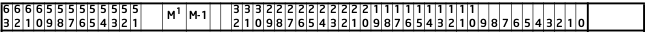
\includegraphics[width=14cm]{../vm/pte-tbl-top}};
\node[below=-.5mm of tp,inner sep=0mm] {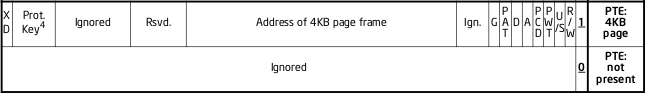
\includegraphics[width=14cm]{../vm/pte-tbl-bottom}};
\end{tikzpicture}
\begin{itemize}
    \small
    \item present = valid\tikzmark{present}
    \item R/W = writes allowed?
    \item U/S = user-mode allowed? (``user/supervisor'')
    \item XD = execute-disable?
    \item A = accessed?\tikzmark{accessed} (MMU sets to 1 on page read/write)
    \item D = dirty?\tikzmark{dirty} (MMU sets to 1 on page write)
\end{itemize}
\begin{tikzpicture}[overlay,remember picture]
    \begin{visibleenv}<all:2>
    \node[my callout=accessed,anchor=south west] at ([xshift=-2cm,yshift=-1cm]pic cs:accessed) {
        helps support replacement policies for swapping
    };
    \end{visibleenv}
    \begin{visibleenv}<all:3>
    \node[my callout=dirty,anchor=south west] at ([xshift=-2cm,yshift=-1cm]pic cs:dirty) {
        helps support writeback policy for swapping
    };
    \end{visibleenv}
\end{tikzpicture}
\end{frame}

\begin{frame}{x86-64 page table entries (2)}
\begin{tikzpicture}
\node[inner sep=0mm] (tp) {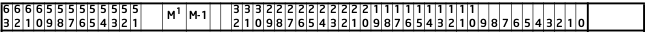
\includegraphics[width=14cm]{../vm/pte-tbl-top}};
\node[below=-.5mm of tp,inner sep=0mm] {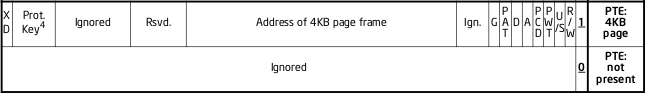
\includegraphics[width=14cm]{../vm/pte-tbl-bottom}};
\end{tikzpicture}
\begin{itemize}
    \small
\item G = global?\tikzmark{global} (shared between all page tables)
\item PWT, PCD, PAT = control how caches work when accessing physical page:
    \begin{itemize}
    \item can disable using the cache entirely
    \item can disable write-back (use write-through instead)
    \item multicore-related cache settings
    \item (and some other settings)
    \end{itemize} 
\end{itemize}
\begin{tikzpicture}[overlay,remember picture]
    \begin{visibleenv}<all:2>
    \node[my callout=global,anchor=south west] at ([xshift=-2cm,yshift=-1cm]pic cs:global) {
        CPU won't evict TLB entries on most page table base registers changes
    };
    \end{visibleenv}
\end{tikzpicture}
\end{frame}



\subsection{exercise: splitting for TLBs}
\subsubsection{3}

\begin{frame}{address splitting exercise (3)}
\begin{itemize}
\item 384-entry, 3-way set-associative TLB
\item 32-bit virtual address; 8KB pages
\item 2-level page table; 4 byte PTEs
    \begin{itemize}
    \item \maybeEmph<5>{256} entries in first level; \maybeEmph<6>{2048} in second
    \end{itemize}
\item split the address {\tt 0x12345678}
    \begin{itemize}
    \item<2-> {\tt \maybeEmph<4>{\maybeEmph<5>{\maybeEmph<8>{0001 0010}} \maybeEmph<6>{\maybeEmph<8>{0011} \maybeEmph<7>{0100  010}}}\maybeEmph<3>{1 0110 0111 1000}}
    \iftoggle{heldback}{}{
    \item<3-> 13-bit page offset \myemph<3>{\tt 1 0110 0111 1000}
    \item<4-> $32-13=19$-bit VPN \myemph<4>{\tt 0001 0010 0011 0100 010}
    \item<5-> 8-bit first part of VPN \myemph<5>{\tt 0001 0010}
    \item<6-> 11-bit second part of VPN \myemph<6>{\tt 0011 0100 010}
    \item<7-> 7-bit TLB index \myemph<7>{0100 010}
    \item<8-> $19-7=12$-bit TLB tag \myemph<8>{0001 0010 0011}
    }
    \end{itemize}
\end{itemize}
\end{frame}


\section{overlapping TLB and cache accesses}
\usetikzlibrary{arrows.meta,circuits.logic.US,fit,matrix,patterns}

\begin{frame}{TLBs and performance}
\begin{tikzpicture}
\tikzset{
    stage/.style={thick,draw,minimum width=2cm,minimum height=2cm},
    >=Latex,
    connect/.style={->,very thick},
}
\node[stage] (tlb) {TLB};
\node[right=1cm of tlb,stage] (l1d) {L1 cache};
\draw[connect] ([xshift=-1cm]tlb.west) -- (tlb);
\draw[connect] (tlb) -- (l1d);
\draw[connect] (l1d) -- ([xshift=1cm]l1d.east);

\draw[<->] ([yshift=-1mm]tlb.south east) -- ([yshift=-1mm]tlb.south west)
    node[below,midway] { extra time? };
\end{tikzpicture}
\end{frame}

\begin{frame}{L1 caches and page numbers (Intel Skylake)}
\begin{tikzpicture}
\tikzset{
    ht/.style={draw,thick,minimum height=1.2cm,align=center,inner sep=0mm},
}

\node[ht,minimum width=12cm] (addr) { physical address \\ (48 bits) };
\node[ht,minimum width=7cm,anchor=north west,alt=<2>{red}] (ppn) at ([yshift=-.1cm]addr.south west){ PPN \\ (36 bit) };
\node[ht,right=0cm of ppn,minimum width=5cm] {page offset \\  (12 bit)};
\node[ht,minimum width=7cm,anchor=north west,alt=<2>{red}] (skylakeTag) at ([yshift=-.1cm]ppn.south west){ L1 cache tag \\ (36 bit) };
\node[ht,minimum width=2.5cm,right=0cm of skylakeTag] (skylakeIndex) { L1 index \\ (6 bit) };
\node[ht,minimum width=2.5cm,right=0cm of skylakeIndex] (skylakeOff) { L1 offset \\ (6 bit) };

\end{tikzpicture}
\begin{itemize}
\item<2-> not a coincidence
\item<2-> why did Intel make this decision?
\end{itemize}
\end{frame}

\begin{frame}{overlapping TLB and cache access}
\begin{tikzpicture}[circuit logic US]
\tikzset{
    myline/.style={-latex,thick},
    myline thin/.style={-latex,thin},
    myline bus/.style={-latex,ultra thick},
    myline no arrow/.style={thick},
    offsetColor/.style={color=yellow!30!black},
    vpnColor/.style={color=yellow!50!black},
    tagColor/.style={color=green!60!black},
    tagStoreFill/.style={fill=green!20},
    tagColorFill/.style={tagColor,fill=green!60!black},
    dataColor/.style={color=blue!60!black},
    dataColorFill/.style={tagColor,fill=blue!60!black},
    dataStoreFill/.style={fill=blue!20},
    triangle down/.style = {draw,regular polygon, regular polygon sides=3, shape border rotate=180},
}
\matrix[tight matrix,
        nodes={draw,
               font=\small\tt,
               text depth=0.2ex,
               text height=1.4ex,
        },
        row 1/.style={nodes={font=\small\bfseries}},
        column 1/.style={nodes={text width=1cm,align=center}},
        column 2/.style={nodes={text width=1cm,tagColor,tagStoreFill}},
        column 3/.style={nodes={text width=1.3cm,dataColor,dataStoreFill}},
        column 4/.style={nodes={text width=.1cm,draw=none}},
        column 5/.style={nodes={text width=1cm,align=center}},
        column 6/.style={nodes={text width=1cm,tagColor,tagStoreFill}},
        column 7/.style={nodes={text width=1.3cm,dataColor,dataStoreFill}},
        ] (cache) {
    valid \& tag \&  data \& ~ \& valid \& tag \& data\\
    1  \& 10 \& 00 11 \& ~ \& 1 \& 00 \& AA BB \\
    ~ \& ~ \& ~ \&   ~ \&  ~ \& ~ \& ~\\
    ~ \& ~ \& ~ \&   ~ \&  ~ \& ~ \& ~\\
    ~ \& ~ \& ~ \&   ~ \&  ~ \& ~ \& ~\\
    1 \&  11 \& B4 B5 \& ~ \& 1 \& 01 \& 33 44 \\
    ~ \& ~ \& ~ \&   ~ \&  ~ \& ~ \& ~\\
    ~ \& ~ \& ~ \&   ~ \&  ~ \& ~ \& ~\\
    ~ \& ~ \& ~ \&   ~ \&  ~ \& ~ \& ~\\
};
\begin{scope}[every node/.style={draw,rectangle,dashed,inner xsep=0pt,outer sep=0pt,font=\tt}]
\node (idx) at ([yshift=.5cm,xshift=-.3cm]cache.north west){100};
\node[left=0cm of idx,vpnColor] (vpn) {000111};
\node[right=0cm of idx,offsetColor] (offset) {1};
\end{scope}

\node[draw,fill=orange!90!black,below=1.5cm of vpn] (tlb) {TLB};

\node[draw,tagColor,below=1cm of tlb] (tag) {11};

\draw[thick,dashed,-latex,vpnColor] (vpn) -- (tlb) node[near start,font=\small,fill=white]{VPN};
\draw[thick,dashed,-latex,tagColor] (tlb) -- (tag);

\draw[thick,dashed,-latex] (idx) |- (cache-6-1.west) node[near start,font=\small,fill=white,inner sep=2pt,xshift=-.3cm] {index};

%\begin{visibleenv}<2->
    \node[below=0.3cm of cache-9-2,draw,circle,inner sep=3pt] (comp1) {\small =};
    \node[below=1.4cm of cache-9-6,draw,circle,inner sep=3pt] (comp2) {\small =};
    %\coordinate(comp1Intersect) at ($(comp1) + (-.7cm,0.5cm)$);
    %\node[draw,circle,tagColorFill,inner sep=0pt,minimum width=1mm] at (comp1Intersect) {};
    \draw[tagColor,myline] (cache-9-2) -- (comp1);
    \draw[tagColor,myline] (cache-9-6) -- (comp2);

    %\draw[myline no arrow,tagColor] (tag) |- (comp1Intersect);
    %\draw[myline,tagColor] (comp1Intersect) |- (comp1);
    \draw[tagColor,myline] (tag) |- (comp2);
    \draw[tagColor,myline] (tag) |- (comp1) node[near start,font=\small,fill=white] {tag=PPN};
    %\draw[myline no arrow,tagColor] (comp1Intersect) |- (comp2Intersect);
    %\draw[myline,tagColor] (comp2Intersect) |- (comp2);

    \node[xshift=-.4cm,draw,below=1cm of cache-9-3,and gate,logic gate inputs=nn,label={[font=\scriptsize]center:AND}] (validCheck1) {};
    \node[xshift=-.4cm,draw,below=2.0cm of cache-9-7,and gate,logic gate inputs=nn,label={[font=\scriptsize]center:AND}] (validCheck2) {};
    \draw[myline] (comp1.south) |- (validCheck1.input 1);
    \draw[myline] (cache-9-1.south) |- (validCheck1.input 2);
    \draw[myline] (comp2.south) |- (validCheck2.input 1);
    \draw[myline] (cache-9-5.south) |- (validCheck2.input 2);
%\end{visibleenv}

\begin{visibleenv}<3->
\node[fit=(cache-6-1) (cache-6-7),inner sep=1pt,red,draw,line width=1pt] {};
\end{visibleenv}

%\node[draw,trapezium,inner xsep=0pt,outer sep=0pt,trapezium angle=75,below=.7cm of validCheck2,
%text width=5cm,shape border rotate=180,xshift=1.5cm] (mux) {};
%\draw[myline] (validCheck1.output) -| (buffer1.west);
%\draw[myline] (cache-9-3.south) -- (buffer1);
%\draw[myline] (buffer1.south) -- (bufEnd1);
\coordinate (outputData) at ([xshift=1.5cm,yshift=-.5cm]cache-9-7.south east);
\coordinate (beforeOutputData) at ([xshift=-.5cm]outputData);
\coordinate (outputHit1) at ([xshift=-1.5cm] beforeOutputData |- validCheck1.output);
\coordinate (outputHit2) at ([xshift=-1.5cm] beforeOutputData |- validCheck2.output);
%\begin{visibleenv}<2->
\node[or gate,logic gate inputs=nn,label={[font=\scriptsize]center:OR},anchor=output] (validCheckTotal)
    at ([xshift=1cm]$(outputHit1)!0.5!(outputHit2)$) {};
%\draw[myline] (validCheck1.output) -- (outputHit1) |- (validCheckTotal.input 1);
    \draw[myline no arrow] (validCheck1.output) -- ([xshift=-1pt]validCheck1.output -| cache-9-5.south);
    \draw[myline no arrow] ([xshift=1pt]validCheck1.output -| cache-9-5.south) -- 
                  ([xshift=-2pt]validCheck1.output -| cache-9-6.south);
    \draw[myline no arrow] ([xshift=2pt]validCheck1.output -| cache-9-6.south) -- (outputHit1);
    \draw[myline] (outputHit1) |- (validCheckTotal.input 1);
\draw[myline] (validCheck2.output) -- (outputHit2) |- (validCheckTotal.input 2);
\draw[myline] (validCheckTotal.output) -- ++(.5cm,0cm) node[right] {is hit? ({\tt 1})};
%\end{visibleenv}
%\begin{visibleenv}<3->
    \node[dataColor,draw,minimum width=.5cm,minimum height=1cm,mux,anchor=east,inputs=nn] (outputSelect) at ([xshift=-.2cm]beforeOutputData) {};
    \draw[myline] (outputHit1) -| (outputSelect.south);
    \fill[black] (outputHit1) circle (2pt);
    %\draw[myline,dataColor] (cache-9-3.south) |- (outputSelect.input 2);
        \draw[dataColor,myline no arrow] (cache-9-3.south) |- ([xshift=-1pt]cache-9-5.south |- outputSelect.input 2);
        \draw[dataColor,myline no arrow] ([xshift=1pt]cache-9-5.south |- outputSelect.input 2) --
                               ([xshift=-1pt]cache-9-6.south |- outputSelect.input 2);
        \draw[dataColor,myline] ([xshift=1pt]cache-9-6.south |- outputSelect.input 2) --
                               (outputSelect.input 2);
    \draw[myline,dataColor] (cache-9-7.south) |- (outputSelect.input 1);
    \draw[myline no arrow,dataColor] (outputSelect.output) -- (beforeOutputData);
    \node[draw,minimum width=.5cm,minimum height=1cm,mux,anchor=west,inputs=nn] (selectByte) at (outputData) {};
    \foreach \x in {1,2} {
        \draw[dataColor,myline thin] (beforeOutputData) |- (selectByte.input \x);
    };
    \draw[offsetColor,myline] (offset.east) -| (selectByte.north) node[very near start,fill=white,font=\small] {offset};
    \draw[dataColor,myline thin] (selectByte.output) -- ++(0.5cm,0cm) -- ++(0cm,0.5cm) node[above,align=center] {data\\({\tt B5})};
%\end{visibleenv}

\begin{visibleenv}<2>
\node[fit=(tlb),draw,red, ultra thick] {};
\node[my callout2=tlb.east] at ([xshift=1cm]tlb.east) {
    perform TLB access \myemph{while cache access is happening}
};
\end{visibleenv}

\end{tikzpicture}
\end{frame}

\begin{frame}{virtually-indexed, physically-tagged}
\begin{itemize}
    \item called virtually-indexed, physically-tagged cache
    \item requirement: \myemph{index contained entirely in page offset}
        \begin{itemize}
        \item do not need to do translation to start cache access
        \end{itemize}
    \item tag overlaps with PPN
        \begin{itemize}
        \item example: tag=PPN
        \item (but tag could include part of page offset, too)
        \end{itemize}
    \item do TLB access \myemph{while retrieving cache set}
    \vspace{.5cm}
    \item most common design in current processors
    \item reason for highly associative (e.g. 8-way) L1 caches
\end{itemize}
\end{frame}


\subsection{exercise}
\begin{frame}{address splitting}
\begin{itemize}
    \item 16-bit virtual addresses
    \item 64-byte pages
    \vspace{.5cm}
    \item 256B, 8-way L1 cache with 16B blocks
    \vspace{.5cm}
    \item can TLB and cache access overlap?
\end{itemize}
\end{frame}


\subsection{alternative: virtual caches}
\usetikzlibrary{positioning}

\begin{frame}{physical caches}
\begin{itemize}
    \item so far: caches use \myemph{physical addresses}:
    \item means cache lookup can't complete without TLB
        \begin{itemize}
        \item (and can't start without index from physical address)
        \end{itemize}
    \end{itemize}
\begin{tikzpicture}
\tikzset{
    >=Latex,
    box/.style={minimum height=2cm,minimum width=2cm,draw,thick},
    myline/.style={->,ultra thick},
}
\node (memA) {memory address};
\node[box,right=1cm of memA] (tlb) {TLB};
\node[box,right=1cm of tlb] (l1) {L1 cache};
\draw[myline] (memA) -- (tlb);
\draw[myline] (tlb) -- (l1);
\draw[myline,dotted] (memA.north) -- ++(0cm,1.5cm) -| (l1) node[midway,fill=white] {page offset};
\end{tikzpicture}
\end{frame}

\begin{frame}{virtual indexing}
\begin{itemize}
\item alternate option: have caches hold virtual addresses \textit{and match tags} with virtual addresses
\item advantage: don't need to wait for TLB lookup at all
\end{itemize}
\begin{tikzpicture}
\tikzset{
    >=Latex,
    box/.style={minimum height=2cm,minimum width=2cm,draw,thick},
    myline/.style={->,ultra thick},
}
\node (memA) {memory address};
\node[box,right=1cm of memA] (l1) {L1 cache};
\node[box,right=3cm of l1] (tlb) {TLB};
\draw[myline] (memA) -- (l1);
\draw[myline,dotted] (l1)-- (tlb) node[midway,fill=white] {on miss};
\node[box,right=1cm of tlb] (l2) {L2 cache};
\draw[myline] (tlb) -- (l2);
\end{tikzpicture}
\begin{itemize}
\item but some things more complicated:
\begin{itemize}
    \item need to invalidate caches on page table changes
    \item need to deal multiple VPNs for same physical page (``aliasing'')
\end{itemize}
\end{itemize}
\end{frame}



\usetikzlibrary{arrows.meta,matrix,positioning}

% FIXME: explain we are using VIRTUAL TAGS
% FIXME: explain aliasing problem with one set
\begin{frame}{virtual caches: aliasing problem}
    \begin{itemize}
        \item two virtual addresses can map to same physical
        \item problem for caches with virtual indexes+tags
        \vspace{.5cm}
        \item say VA 0x1000 and 0x2000 map to same physical
        \item what happens if application writes to 0x1000
        \item \ldots then reads from 0x2000?
    \end{itemize}
\end{frame}

\begin{frame}{virtual cache aliasing solutions}
    \begin{itemize}
    \item software solution: OS promises not to have aliasing
    \item hardware solution: hardware detects aliasing
        \begin{itemize}
        \item requires extra bookkeeping
        \end{itemize}
    \end{itemize}
\end{frame}

\begin{frame}[fragile,label=hwAlias]{hardware alias detection (1)}
    \begin{itemize}
    \item key idea: store physical address \textit{and virtual-address-based tag}
    \item store value? check for other copies of same physical addr
    \item if found: evict other copies
    \end{itemize}
\begin{tikzpicture}
\tikzset{
    v/.style={visible on=<#1->,alt=<#1>{red}},
    h/.style={alt=<#1>{red}},
    tagColor/.style={color=green!60!black},
    physColor/.style={color=red!60!black},
    dataColor/.style={color=blue!60!black},
    offsetColor/.style={color=yellow!30!black},
}
\matrix[tight matrix,
        nodes={font=\small\tt,text depth=.1ex,text height=1ex,minimum height=.5cm},
        row 1/.append style={nodes={font=\small\bfseries,minimum height=.5cm}},
        column 1/.append style={nodes={draw=none,text width=1.2cm}},
        column 2/.append style={nodes={align=center,text width=.5cm}},
        column 3/.append style={nodes={align=center,tagColor,text width=2cm}},
        column 4/.append style={nodes={align=center,physColor,text width=2cm}},
        column 5/.append style={nodes={text width=1cm,align=center,dataColor}},
        column 6/.append style={nodes={draw=none,text width=.1cm}},
        column 7/.append style={nodes={align=center,text width=.5cm}},
        column 8/.append style={nodes={align=center,tagColor,text width=2cm}},
        column 9/.append style={nodes={align=center,physColor,text width=2cm}},
        column 10/.append style={nodes={text width=1cm,align=center,dataColor}},
       ] (cache)  {
           index \& V \& tag \& phys addr \& value \& ~ \& V \& tag \& phys addr \& value \\
0\&
    % i 0, 0:
    1 \& 
    0x03312 \&
    0x1F4300 \&
    \ldots \&  ~ \&
    % i 0, 1:
    1 \&
    0x03311 \&
    0x1F3400 \&
    \ldots \\
1\& 
    % i 1, 0:
    1 \&
    0x7FF33 \&
    0x183220 \&
    \ldots \& ~ \& 
    % i 1, 1:
    1 \&
    0x03310 \&
    0x0F3A20 \&
    \ldots \\
2\& 
    % i 1, 0:
    1 \&
    0x7FF33 \&
    0x183240 \&
    \ldots \& ~ \& 
    % i 1, 1:
    1 \&
    0x03320 \&
    0x030040 \&
    \ldots \\
\ldots \\
};
\end{tikzpicture}
\end{frame}

\begin{frame}{checking all the physical addresses? (1)}
    \begin{itemize}
    \item scanning entire cache for same physical address?
    \item do we really need to scan everything?
    \vspace{.5cm}
\item<2-> exercise(1): if we have 4096 ($2^{12}$) byte pages, give an example of a virtual address that could
          map to the same physical as \texttt{0x12010}?
    \iftoggle{heldback}{}{
    \item<3-> must have same page offset, so 0x0010, 0x1010, 0x2010, 0x3010, etc.
    }
    \end{itemize}
\end{frame}
\begin{frame}{checking all the physical addresses? (2)}
    \begin{itemize}
    \item scanning entire cache for same physical address?
    \item do we really need to scan everything?
    \vspace{.5cm}
    \item with 4K pages ($2^{12}$ byte):
    \item exercise(2): if we have a direct-mapped 4K \textbf{virtual} cache with 16 byte blocks,
          in which sets can be these aliasing addresses be stored?
    \end{itemize}
\begin{tikzpicture}
\tikzset{
    ht/.style={draw,thick,minimum height=1.2cm,align=center,inner sep=0mm},
}
\node[ht,minimum width=8cm,anchor=north west] (ppn) { PPN };
\node[ht,minimum width=7cm,anchor=north east] (vpn) at ([yshift=-.1cm]ppn.south east){ VPN };
\node[ht,right=0cm of ppn,minimum width=6cm] {page offset};
\node[ht,right=0cm of vpn,minimum width=6cm] {page offset};
\node[ht,minimum width=7cm,anchor=north west] (cacheTag) at ([yshift=-.1cm,xshift=0cm]vpn.south west){ cache tag };
\node[ht,minimum width=3.5cm,right=0cm of cacheTag] (cacheIndex) { cache index };
\node[ht,minimum width=2.5cm,right=0cm of cacheIndex] (cacheOff) { cache offset };
\end{tikzpicture}
\end{frame}

\begin{frame}{checking all the physical addresses? (3)}
    \begin{itemize}
    \item scanning entire cache for same physical address?
    \item do we really need to scan everything?
    \vspace{.5cm}
    \item exercise(3): if we have a direct-mapped \textbf{8K} \textbf{virtual} cache with 16-byte blocks,
         in which sets can these aliasing addresses be stored?
    \end{itemize}
\begin{tikzpicture}
\tikzset{
    ht/.style={draw,thick,minimum height=1.2cm,align=center,inner sep=0mm},
}

\node[ht,minimum width=8cm,anchor=north west] (ppn) { PPN };
\node[ht,minimum width=7cm,anchor=north east] (vpn) at ([yshift=-.1cm]ppn.south east){ VPN };
\node[ht,right=0cm of ppn,minimum width=5cm] {page offset};
\node[ht,right=0cm of vpn,minimum width=5cm] {page offset};
\node[ht,minimum width=6cm,anchor=north west] (cacheTag) at ([yshift=-.1cm,xshift=0cm]vpn.south west){ cache tag };
\node[ht,minimum width=3.5cm,right=0cm of cacheTag] (cacheIndex) { cache index };
\node[ht,minimum width=2.5cm,right=0cm of cacheIndex] (cacheOff) { cache offset };
\begin{visibleenv}<2>
    \draw[red,dotted,line width=4pt] (vpn.north east |- ppn.north) rectangle (cacheIndex.south west);
\end{visibleenv}
\end{tikzpicture}
\end{frame}

\begin{frame}{virtual caches: detecting aliasing}
    \begin{itemize}
    \item suppose two virtual addresses with same physical address
    \item addrs differ only VPN bits
    \item finding which indexes to check: worry about overlap:
    \end{itemize}
\begin{tikzpicture}
\tikzset{
    ht/.style={draw,thick,minimum height=1.2cm,align=center,inner sep=0mm},
}

\node[ht,minimum width=8cm,anchor=north west] (ppn) { PPN };
\node[ht,minimum width=7cm,anchor=north east] (vpn) at ([yshift=-.1cm]ppn.south east){ VPN };
\node[ht,right=0cm of ppn,minimum width=5cm] {page offset};
\node[ht,right=0cm of vpn,minimum width=5cm] {page offset};
\node[ht,minimum width=6cm,anchor=north west] (cacheTag) at ([yshift=-.1cm,xshift=0cm]vpn.south west){ cache tag };
\node[ht,minimum width=3.5cm,right=0cm of cacheTag] (cacheIndex) { cache index };
\node[ht,minimum width=2.5cm,right=0cm of cacheIndex] (cacheOff) { cache offset };
\begin{visibleenv}<2>
    \draw[red,dotted,line width=4pt] (vpn.north east |- ppn.north) rectangle (cacheIndex.south west);
\end{visibleenv}
\end{tikzpicture}
\end{frame}

\begin{frame}{virtual caches: aliasing detection outline}
    \begin{itemize}
    \item hardware alias detection mechanism
    \vspace{.5cm}
    \item store physical address of each block in the cache
        \begin{itemize}
            \item \ldots in addition to virtual tag
        \end{itemize}
    \item when adding value to cache, try \myemph{all other indexes for same page offset}
    \item if any match physical address: evict that copy
    \item result: only store one virtual address per physical address at a time
    \item actual strategy used by AMD Opteron's instruction cache
        \begin{itemize}
        \item 2 cache index bits overlapping VPN
        \item 4 cache sets to check on cache replacement
        \item (also on conflicting writes to data cache?)
        \end{itemize}
    \end{itemize}
\end{frame}

% FIXME: example of virtual caches
% FIXME: example of antialiasing mechanism

\section{i7 memory}
\begin{frame}{book's diagram}
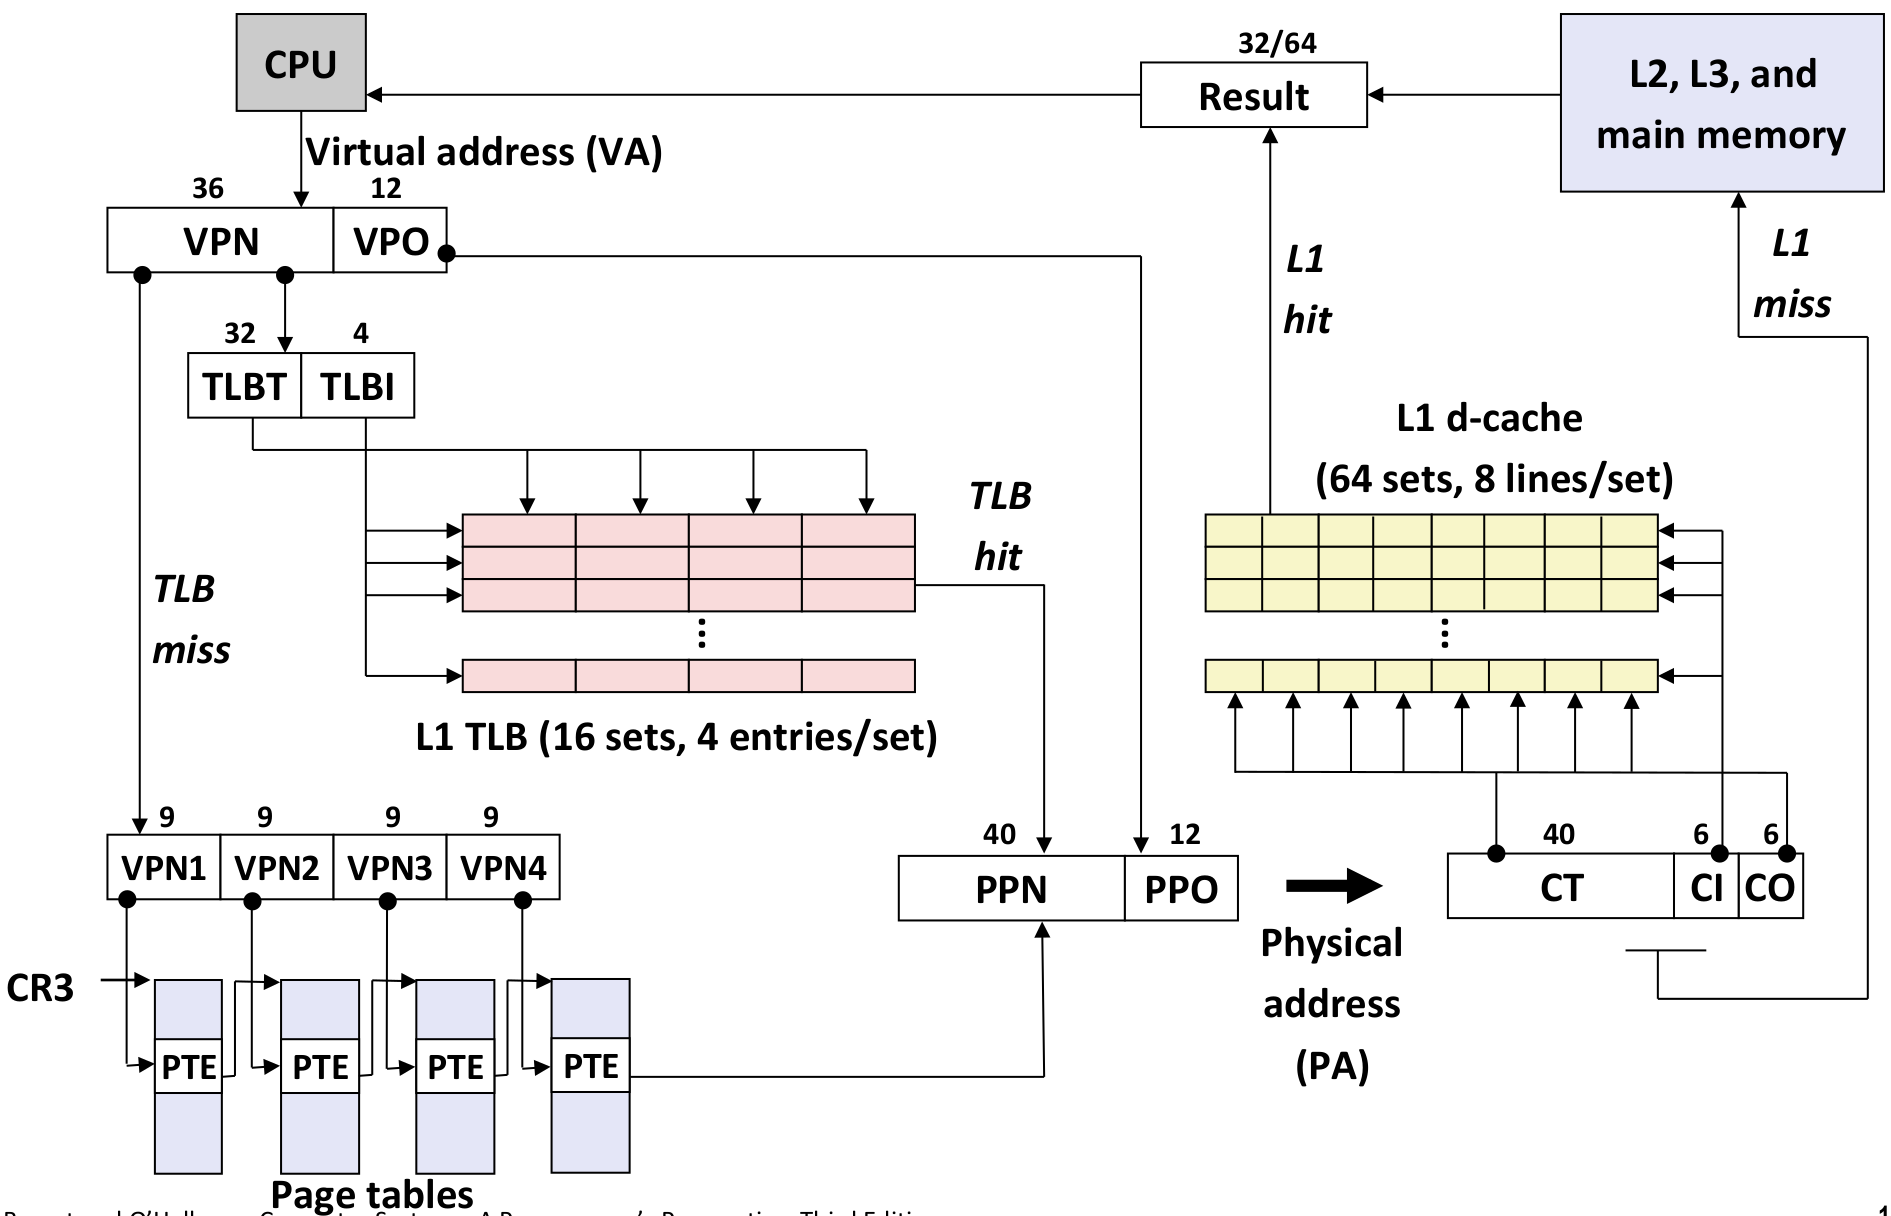
\includegraphics[height=0.9\textheight]{../vm/i7-diag}
\end{frame}


\section{huge pages}

\begin{frame}{are pages too small?}
    \begin{itemize}
    \item program accessing a lot of memory? lots of TLB entries
        \begin{itemize}
        \item lots of TLB misses
        \item lots of space for page tables
        \end{itemize}
    \item often, really like larger pages,\ldots
    \item but not all the time
        \begin{itemize}
        \item still want to be able to allocate small amounts of memory to small programs
        \item want to load/store small amounts of data from disk
        \end{itemize}
    \item common to provide variable-sized pages for OS
    \end{itemize}
\end{frame}

\begin{frame}{``huge pages''}
\begin{tikzpicture}
    \tikzset{
        addrPart/.style={draw,minimum height=.6cm},
        pt/.style={draw,ultra thick,minimum height=2cm,minimum width=3.25cm,align=center},
        pte/.style={draw,thin,minimum height=.6cm,minimum width=3.25cm,font=\small,fill=black!5},
        pteX/.style={draw,thin,minimum height=.6cm,minimum width=3.25cm,font=\fontsize{11}{11}\selectfont,fill=black!5},
        >=Latex,
        compute/.style={thick,->},
        computeB/.style={thick,->,dashed},
        computeR/.style={thick,->,red},
    }
    \node[addrPart,minimum width=4.25cm] (vpn1) {VPN part 1};
    \node[addrPart,right=0cm of vpn1,minimum width=4.25cm] (vpn2) {VPN part 2};
    \node[addrPart,right=0cm of vpn2,minimum width=5cm] (po) {(normal) page offset};

    \node[pt,below=0.25cm of vpn1,xshift=1cm] (first) {
    };
    
    \node[draw,anchor=east] (ptbr) at ([xshift=-.5cm,yshift=.25cm]first.south west) {PTBR};
    \draw[compute] (ptbr.east) -- ++(.1cm,0cm) |- (first.south west);
    \node[pteX] (pte1) at ([yshift=1.3cm]first.south) {page table entry~~~~};
    \node[fill=yellow!50!white,font=\small,anchor=east] at (pte1.east) {0};
    \draw[computeB] ([xshift=1.2cm]vpn1.south west) |- (pte1.south west);

    \node[pt,below=0.25cm of vpn2,xshift=1cm] (second) {
    };
    
    \draw[compute] (pte1.east) -- ++(.25cm,0cm) |- (second.south west);
    
    \node[pte] (pte2) at ([yshift=0.8cm]second.south) {page table entry};
    \draw[computeB] ([xshift=1.2cm]vpn2.south west) |- (pte2.south west);
    
    \node[pt,below=.25cm of po,xshift=1cm] (final) {
        physical page \\ (normal)
    };
    \draw[compute] (pte2.east) -- ++(.25cm,0cm) |- (final.south west);
    \draw[computeB] ([xshift=1.2cm]po.south west) |- ([yshift=1.5cm]final.south west);

    \node[addrPart,minimum width=4.25cm,below=2.5cm of vpn1] (vpn1B) {VPN part 1};
    \node[addrPart,minimum width=9.25cm,right=0cm of vpn1B] (vpn2B) {``huge page'' page offset};

    \node[pt,below=1.25cm of first] (firstB) {};
    \node[draw,anchor=east] (ptbrB) at ([xshift=-.5cm,yshift=.25cm]firstB.south west) {PTBR};
    \node[pt,overlay,minimum height=5cm,below=1.25cm of final] (finalB) {
            physical page \\ (huge)
    };
    
    \draw[compute] (ptbrB.east) -- ++(.1cm,0cm) |- (firstB.south west);
    
    \node[pteX] (pte1B) at ([yshift=1.3cm]firstB.south) {page table entry~~~};
    \node[fill=yellow!50!white,font=\small,anchor=east] at (pte1B.east) {1};
    \draw[compute] (pte1B.east) -- ++ (4.5cm, 0cm) |- (finalB.south west);
    \draw[computeB] ([xshift=-3.75cm]vpn2B.south east) |- ([yshift=1.5cm]finalB.south west);
\end{tikzpicture}
\end{frame}

\begin{frame}{big pages on x86-64}
\begin{itemize}
\item option for 2MB or 1GB pages instead of 4KB pages
\item first, second, third-level page table entries can point to either
    \begin{itemize}
    \item next page table (normal case), or
    \item a ``huge page'' 
    \end{itemize}
\item big changes to TLB needed?
    \begin{itemize}
    \item Intel/AMD don't seem to disclose what they do,\ldots
    \item but seems like Intel has a special cache for non-fourth(last)-level PTEs
    \item (which speeds up page tabe lookup for normal pages)
    \item and use this for `huge page' PTEs, too
    \end{itemize}
    \vspace{1cm}
\item processes can have mix of huge and normal apges
\end{itemize}
\end{frame}

\begin{frame}{why big pages?}
\begin{itemize}
\item TLB misses can create same sort of problems as cache misses
\item can do cache blocking to help with TLB misses but\ldots
    \vspace{.5cm}
\item big pages are relatively easy to implement
\item might dramatically reduce TLB misses
\end{itemize}
\end{frame}


\subsection{space saving or not with multi-level}
\usetikzlibrary{arrows.meta,matrix}

\begin{frame}{page table space exercise (1)}
\begin{itemize}
\item 4-level page table
\item 512 PTEs of 8 bytes each for each page table
\vspace{.5cm}
\item suppose a process has exactly one page allocated
\item how much space for page tables?
\iftoggle{heldback}{}{
    \item<2-> 1 page at each level (4KB each)
    \item<2-> exactly one valid entry in each of them
}
\end{itemize}
\end{frame}

\begin{frame}{page table space exercise (1)}
\iftoggle{heldback}{}{
\begin{tikzpicture}
    \tikzset{
        >=Latex,
        used/.style={fill=green},
        connect/.style={very thick,->},
        tight matrix/.append style={inner sep=1mm,draw,thick,nodes=thin},
    },
    \matrix[tight matrix] (first) {
        ~ \\
        ~ \\
        |[used,alias=firstAlloc]| ~ \\
        ~ \\
        ~ \\
        ~ \\
        |[draw=none]| \ldots \\
    };
    \matrix[tight matrix,right=1cm of first] (second) {
        ~ \\
        ~ \\
        ~ \\
        ~ \\
        |[used,alias=secondAlloc]| ~ \\
        ~ \\
        |[draw=none]| \ldots \\
    };
    \matrix[tight matrix,right=1cm of second] (third) {
        ~ \\
        |[used,alias=thirdAlloc]| ~ \\
        ~ \\
        ~ \\
        ~ \\
        ~ \\
        |[draw=none]| \ldots \\
    };
    \matrix[tight matrix,right=1cm of third] (fourth) {
        ~ \\
        ~ \\
        ~ \\
        ~ \\
        |[used,alias=fourthAlloc]| ~ \\
        ~ \\
        |[draw=none]| \ldots \\
    };
    \draw[connect] (firstAlloc.east) -- ++(.5cm,0cm) |- (second-1-1.west);
    \draw[connect] (secondAlloc.east) -- ++(.5cm,0cm) |- (third-1-1.west);
    \draw[connect] (thirdAlloc.east) -- ++(.5cm,0cm) |- (fourth-1-1.west);
    \draw[connect] (fourthAlloc) -- ++(1cm, 0cm) node[right] {the one page};
    \node[below=.25cm of first] {1 page table};
    \node[below=.25cm of second] {2};
    \node[below=.25cm of third] {3};
    \node[below=.25cm of fourth] {4};
    \node[align=left,below=2cm of fourth] { \myemph{4 page tables} at 1 page/page table \\ plus 1 page of data \\ 5 pages total };
\end{tikzpicture}
}
\end{frame}

\begin{frame}{page table space exercise (2)}
\begin{itemize}
\item 4-level page table
\item 512 PTEs of 8 bytes each for each page table
\vspace{.5cm}
\item suppose a process has exactly two pages allocated:
    \begin{itemize}
    \item one at address 0x0, one at address {\tt 0x20000000000}
    \end{itemize}
\item how much space for page tables?
\iftoggle{heldback}{}{
    \item<2-> 1 shared first-level PT, with two valid entries
    \item<2-> two second-level PTs, each with one valid entry
    \item<2-> two third-level PTs, each with one valid entry
    \item<2-> two fourth-level PTs, each with one valid entry
}
\end{itemize}
\end{frame}

\begin{frame}{page table space exercise (2)}
\iftoggle{heldback}{}{
\begin{tikzpicture}
    \tikzset{
        >=Latex,
        used/.style={fill=green},
        connect/.style={very thick,->},
        tight matrix/.append style={inner sep=1mm,draw,thick,nodes=thin},
    },
    \matrix[tight matrix] (first) {
        |[used,alias=firstAlloc]| ~ \\
        ~ \\
        ~ \\
        |[draw=none,align=center]| \ldots \\
        ~ \\
        |[used,alias=firstAllocB]| ~ \\
        ~ \\
        ~ \\
        |[draw=none]| \ldots \\
    };
    \matrix[tight matrix,right=1cm of first] (second) {
        |[used,alias=secondAlloc]| ~ \\
        ~ \\
        ~ \\
        ~ \\
        ~ \\
        ~ \\
        ~ \\
        |[draw=none,align=center]| \ldots \\
    };
    \matrix[tight matrix,below=1cm of second] (secondB) {
        |[used,alias=secondAllocB]| ~ \\
        ~ \\
        ~ \\
        ~ \\
        ~ \\
        ~ \\
        ~ \\
        |[draw=none,align=center]| \ldots \\
    };
    \matrix[tight matrix,right=1cm of second] (third) {
        |[used,alias=thirdAlloc]| ~ \\
        ~ \\
        ~ \\
        ~ \\
        ~ \\
        ~ \\
        ~ \\
        |[draw=none,align=center]| \ldots \\
    };
    \matrix[tight matrix,right=1cm of secondB] (thirdB) {
        |[used,alias=thirdAllocB]| ~ \\
        ~ \\
        ~ \\
        ~ \\
        ~ \\
        ~ \\
        ~ \\
        |[draw=none,align=center]| \ldots \\
    };
    \matrix[tight matrix,right=1cm of third] (fourth) {
        |[used,alias=fourthAlloc]| ~ \\
        ~ \\
        ~ \\
        ~ \\
        ~ \\
        ~ \\
        ~ \\
        |[draw=none,align=center]| \ldots \\
    };
    \matrix[tight matrix,right=1cm of thirdB] (fourthB) {
        |[used,alias=fourthAllocB]| ~ \\
        ~ \\
        ~ \\
        ~ \\
        ~ \\
        ~ \\
        ~ \\
        |[draw=none,align=center]| \ldots \\
    };
    \draw[connect] (firstAlloc.east) -- ++(.5cm,0cm) |- (second-1-1.west);
    \draw[connect] (secondAlloc.east) -- ++(.5cm,0cm) |- (third-1-1.west);
    \draw[connect] (thirdAlloc.east) -- ++(.5cm,0cm) |- (fourth-1-1.west);
    \draw[connect] (fourthAlloc) -- ++(1cm, 0cm) node[right] {page at {\tt 0x0}};

    \draw[connect] (firstAllocB.east) -- ++(.5cm,0cm) |- (secondB-1-1.west);
    \draw[connect] (secondAllocB.east) -- ++(.5cm,0cm) |- (thirdB-1-1.west);
    \draw[connect] (thirdAllocB.east) -- ++(.5cm,0cm) |- (fourthB-1-1.west);
    \draw[connect] (fourthAllocB) -- ++(1cm, 0cm) node[right] {page at {\tt 0x20000000000}};
    %\node[align=left,below=2cm of fourth] { \myemph{7 page tables} at 1 page/page table \\ plus 2 page of data \\ 9 pages total };
\end{tikzpicture}
}
\end{frame}

\begin{frame}{page table space exercise (3)}
\begin{itemize}
\item 4-level page table; each PT: 512 PTEs of 8 bytes
\item suppose a process has 100 pages of stack, 100 pages of code+constants (contiguous)
    \begin{itemize}\item stack and code+constants far apart\end{itemize}
\item how much space for page tables? \only<2->{--- \textit{minimum:}}
\iftoggle{heldback}{}{
    \item<2-> 1 shared first-level PT, with two valid entries
    \item<2-> two second-level PT, each with one valid entry
    \item<2-> two third-level PT, each with one valid entry
    \item<2-> two fourth-level PT, each with 100 valid entries
}
\end{itemize}
\end{frame}

\begin{frame}{page table space exercise (3)}
\iftoggle{heldback}{}{
\begin{tikzpicture}
    \tikzset{
        >=Latex,
        used/.style={fill=green},
        connect/.style={very thick,->},
        tight matrix/.append style={inner sep=1mm,draw,thick,nodes=thin},
    },
    \matrix[tight matrix] (first) {
        ~ \\
        |[draw=none,align=center]| \ldots \\
        ~ \\
        |[used,alias=firstAlloc]| ~ \\
        ~ \\
        |[draw=none,align=center]| \ldots \\
        ~ \\
        |[used,alias=firstAllocB]| ~ \\
        ~ \\
        |[draw=none]| \ldots \\
    };
    \matrix[tight matrix,right=1cm of first] (second) {
        |[used,alias=secondAlloc]| ~ \\
        ~ \\
        ~ \\
        ~ \\
        ~ \\
        ~ \\
        ~ \\
        |[draw=none,align=center]| \ldots \\
    };
    \matrix[tight matrix,below=1cm of second] (secondB) {
        |[used,alias=secondAllocB]| ~ \\
        ~ \\
        ~ \\
        ~ \\
        ~ \\
        ~ \\
        ~ \\
        |[draw=none,align=center]| \ldots \\
    };
    \matrix[tight matrix,right=1cm of second] (third) {
        |[used,alias=thirdAlloc]| ~ \\
        ~ \\
        ~ \\
        ~ \\
        ~ \\
        ~ \\
        ~ \\
        |[draw=none,align=center]| \ldots \\
    };
    \matrix[tight matrix,right=1cm of secondB] (thirdB) {
        |[used,alias=thirdAllocB]| ~ \\
        ~ \\
        ~ \\
        ~ \\
        ~ \\
        ~ \\
        ~ \\
        |[draw=none,align=center]| \ldots \\
    };
    \matrix[tight matrix,right=1cm of third,nodes={used}] (fourth) {
        |[used,alias=fourthAlloc]| ~ \\
        ~ \\
        ~ \\
        |[draw=none,fill=none,align=center]| \ldots \\
        ~ \\
        |[fill=none]| ~ \\
        |[fill=none]| ~ \\
        |[draw=none,fill=none,align=center]| \ldots \\
    };
    \matrix[tight matrix,right=1cm of thirdB,nodes={used}] (fourthB) {
        ~ \\
        ~ \\
        ~ \\
        |[draw=none,fill=none,align=center]| \ldots \\
        ~ \\
        |[fill=none]| ~ \\
        |[fill=none]| ~ \\
        |[draw=none,fill=none,align=center]| \ldots \\
    };
    \draw[connect] (firstAlloc.east) -- ++(.5cm,0cm) |- (second-1-1.west);
    \draw[connect] (secondAlloc.east) -- ++(.5cm,0cm) |- (third-1-1.west);
    \draw[connect] (thirdAlloc.east) -- ++(.5cm,0cm) |- (fourth-1-1.west);
    \draw[connect] (fourth-1-1.east) -- ++(1cm, 0cm) node[right] {first of 100 pages of code};

    \draw[connect] (firstAllocB.east) -- ++(.5cm,0cm) |- (secondB-1-1.west);
    \draw[connect] (secondAllocB.east) -- ++(.5cm,0cm) |- (thirdB-1-1.west);
    \draw[connect] (thirdAllocB.east) -- ++(.5cm,0cm) |- (fourthB-1-1.west);
    \draw[connect] (fourthB-1-1.east) -- ++(1cm, 0cm) node[right] {first of 100 pages of stack};
    %\node[align=left,below=2cm of fourth] { \myemph{7 page tables} at 1 page/page table \\ plus 2 page of data \\ 9 pages total };
\end{tikzpicture}
}
\end{frame}

\begin{frame}{page table space exercise (3)}
\begin{itemize}
\item 4-level page table; each PT: 512 PTEs of 8 bytes
\item suppose a process has 100 pages of stack, 100 pages of code+constants (contiguous)
\item how much space for page tables? \only<2->{--- \textit{maximum:}}
\iftoggle{heldback}{}{
    \item<2-> 1 shared first-level PT, with four valid entries
    \item<2-> four second-level PT, each with one valid entry
        \begin{itemize}\item two for stack, two for code+constants\end{itemize}
    \item<2-> four third-level PT, each with one valid entry
    \item<2-> four fourth-level PT, each with 50 valid entries
}
\end{itemize}
\end{frame}

\begin{frame}[fragile,label=ptSpaceEx3Pic]{page table space exercise (3)}
\iftoggle{heldback}{}{
\begin{tikzpicture}
    \tikzset{
        >=Latex,
        used/.style={fill=green},
        connect/.style={very thick,->},
        tight matrix/.append style={inner sep=1mm,draw,thick,nodes=thin},
    },
    \matrix[tight matrix] (first) {
        ~ \\
        |[draw=none,align=center]| \ldots \\
        ~ \\
        |[used,alias=firstAllocX]| ~ \\
        |[used,alias=firstAlloc]| ~ \\
        ~ \\
        |[draw=none,align=center]| \ldots \\
        ~ \\
        |[used,alias=firstAllocBX]| ~ \\
        |[used,alias=firstAllocB]| ~ \\
        ~ \\
        |[draw=none]| \ldots \\
    };
    \matrix[tight matrix,above right=-1cm and 2cm of first] (secondX) {
        ~ \\
        |[draw=none,align=center]| \ldots \\
        ~ \\
        |[used,alias=secondAllocX]| ~ \\
    };
    \matrix[tight matrix,below=.5cm of secondX] (second) {
        |[used,alias=secondAlloc]| ~ \\
        ~ \\
        ~ \\
        |[draw=none,align=center]| \ldots \\
    };
    \matrix[tight matrix,right=1cm of second] (third) {
        |[used,alias=thirdAlloc]| ~ \\
        ~ \\
        ~ \\
        |[draw=none,align=center]| \ldots \\
    };
    \matrix[tight matrix,right=1cm of secondX] (thirdX) {
        ~ \\
        |[draw=none,align=center]| \ldots \\
        ~ \\
        |[used,alias=thirdAllocX]| ~ \\
    };
    \matrix[tight matrix,right=1cm of third,nodes={used}] (fourth) {
        |[used,alias=fourthAlloc]| ~ \\
        ~ \\
        |[draw=none,fill=none,align=center]| \ldots \\
        ~ \\
        |[fill=none]| ~ \\
        |[fill=none]| ~ \\
        |[draw=none,fill=none,align=center]| \ldots \\
    };
    \matrix[tight matrix,above=1cm of fourth,nodes={used}] (fourthX) {
        |[fill=none]| ~ \\
        |[draw=none,fill=none,align=center]| \ldots \\
        |[used]| ~ \\
        |[used]| ~ \\
        |[draw=none,fill=none,align=center]| \ldots \\
        |[used]| ~ \\
    };
    \draw[connect] (firstAlloc.east) -- ++(.5cm,0cm) |- (second-1-1.west);
    \draw[connect] (secondAlloc.east) -- ++(.5cm,0cm) |- (third-1-1.west);
    \draw[connect] (thirdAlloc.east) -- ++(.5cm,0cm) |- (fourth-1-1.west);
    \draw[connect] (fourth-1-1.east) -- ++(1cm, 0cm) node[right,align=left] {first of \\ last 50 pages of code};

    \draw[connect] (firstAllocX.east) -- ++(.5cm,0cm) |- (secondX-1-1.west);
    \draw[connect] (secondAllocX.east) -- ++(.5cm,0cm) |- (thirdX-1-1.west);
    \draw[connect] (thirdAllocX.east) -- ++(.5cm,0cm) |- (fourthX-1-1.west);
    \draw[connect] (fourthX-3-1.east) -- ++(1cm, 0cm) node[right,align=left] {first of \\ first 50 pages of code};

    \draw[connect,dotted] (firstAllocBX.east) -- ++(1cm,0cm) |- ++(2cm,-1cm) node[right] {(similar arrangement for stack pages)};
\end{tikzpicture}
}
\end{frame}

% FIXME: picture of this situation

\begin{frame}{page table space exercise (4)}
\begin{itemize}
\item 4-level page table; each PT: 512 PTEs of 8 bytes
\item suppose a process has 200 pages, randomly distributed in PT
\item about how much space for page tables?
\item<2-> about 165 ($\pm \sim 8$) entries in first-level PT
    \begin{itemize}
        \item (some pages randomly share first-level PT entries)
    \end{itemize}
\item<2-> about 165 second-level PTs, 200 third-level, 200 fourth-level
\item<2-> a bit less than 600 page tables --- almost 2400 KB
\end{itemize}
\end{frame}


\subsubsection{part 1}
\usetikzlibrary{matrix}

\begin{frame}{1-level example}
\begin{itemize}
\item 6-bit virtual addresses, 6-bit physical; 8 byte pages, 1 byte PTE
\item page tables 1 page; PTE: 3 bit PPN (MSB), 1 valid bit, 4 other bits;
\item page table base register {\tt 0x20}; translate virtual address {\tt 0x31}
\end{itemize}
\begin{tikzpicture}
\matrix[tight matrix,anchor=north west,
    nodes={text width=2cm,minimum height=0.5cm,font=\small},
    column 1/.style={nodes={draw=none,font=\small\tt,align=right}},
    column 2/.style={nodes={draw,thick,font=\small\tt,text width=2.6cm,align=left}},
    row 1/.style={nodes={draw=none,font=\small\normalfont}},
    ] (memA)  {
    physical addresses \& bytes \\
    0x00-3 \& 00 11 22 33 \\
    0x04-7 \& 44 55 66 77 \\
    0x08-B \& 88 99 AA BB \\
    0x0C-F \& CC DD EE FF \\
    0x10-3 \& 1A 2A 3A 4A \\
    0x14-7 \& 1B 2B 3B 4B \\
    0x18-B \& 1C 2C 3C 4C \\
    0x1C-F \& 1C 2C 3C 4C \\
};
\matrix[tight matrix,anchor=north west,
    nodes={text width=2cm,minimum height=0.5cm,font=\small},
    column 1/.style={nodes={draw=none,font=\small\tt,align=right}},
    column 2/.style={nodes={draw,thick,font=\small\tt,text width=2.6cm,align=left}},
    row 1/.style={nodes={draw=none,font=\normalfont\small}},
    ] (memB) at ([xshift=0cm]memA.north east) {
    physical addresses \& bytes \\
    0x20-3 \& D0 D1 D2 D3 \\
    0x24-7 \& F4 F5 \maybeEmph<2>{F6} F7 \\
    0x28-B \& 89 9A AB BC \\
    0x2C-F \& CD DE EF F0 \\
    0x30-3 \& BA 0A BA 0A \\
    0x34-7 \& CB 0B CB 0B \\
    0x38-B \& DC \maybeEmph<3-4>{0C} DC 0C \\
    0x3C-F \& EC 0C EC 0C \\
};
%\iftoggle{heldback}{}{
\begin{visibleenv}<2->
\node[right=0cm of memB,align=left] {
    {\tt 0x31} = {\tt \myemph<2>{11 0}\myemph<4>{001}} \\
    \textit{PTE addr:} \\
    \texttt{0x20} + 6 \times 1 = {\tt \myemph<2>{0x26}} \\
    \textit{PTE value:} \\
    {\tt \myemph<2>{0xF6}} = {\tt \myemph<3>{111}1 0110} \\
    PPN {\tt \myemph<3>{111}}, valid {\tt 1} \\
    M[{\tt \myemph<3>{111} \myemph<4>{001}}] = \textbf{M[\tt{0x39}]}\\ $\rightarrow$ {\tt 0x0C}
};
\end{visibleenv}
%}
\end{tikzpicture}
\end{frame}


\section{backup slides}
\begin{frame}{backup slides}
\end{frame}

\subsection{mmap}
\begin{frame}[fragile,label=mmap]{mmap}
\lstset{
    language=C,
    style=small
}
\begin{itemize}
\item Linux/Unix has a function to ``map'' a file to memory
\end{itemize}
\begin{lstlisting}
int file = open("somefile.dat", O_RDWR);

    // data is region of memory that represents file
char *data = mmap(..., file, 0);

    // read byte 6 from somefile.dat
char seventh_char = data[6];

   // modifies byte 100 of somefile.dat
data[100] = 'x';
    // can continue to use 'data' like an array
\end{lstlisting}
\end{frame}

\begin{frame}{swapping almost mmap}
\begin{itemize}
    \item access mapped file for first time, read from disk
        \begin{itemize}
        \item (like swapping when memory was swapped out)
        \end{itemize}
    \item write ``mapped'' memory, write to disk eventually
        \begin{itemize}
        \item (like writeback policy in swapping)
        \item use ``dirty'' bit
        \end{itemize}
    \vspace{.5cm}
    \item extra detail: other processes should see changes
        \begin{itemize}
        \item all accesses to file use \myemph{same physical memory}
        \end{itemize}
\end{itemize}
\end{frame}


\subsubsection{copy-on-write?} % FIXME: consider skipping
\begin{frame}{fast copies}
\begin{itemize}
    \item Unix mechanism for starting a new process: \texttt{fork()}
    \item creates a \myemph{copy} of an entire program!
    \item (usually, the copy then calls \texttt{execve} --- replaces itself with another program)
    \vspace{.5cm}
    \item how isn't this really slow?
\end{itemize}
\end{frame}

\begin{frame}{do we really need a complete copy?}
\begin{tikzpicture}
\tikzset{
    mylabel/.style={font=\ttfamily},
    mybox/.style={draw,rectangle,minimum width=7cm,fill=white,inner sep=1mm},
    myhigh/.style={draw,rectangle,line width=1mm, draw=blue!80!black,opacity=.3},
}
\begin{scope}[name prefix=A-]
\node[mybox,minimum height=1cm,pattern=north west lines,pattern color=black!5!white] (kernel) {Used by OS};
\node[above=0cm of kernel] {bash};
\node[mybox, minimum height=.5cm, below=1cm of kernel] (stack) {Stack};
\node[mybox, minimum height=.5cm, below=1cm of stack] (heap) {Heap / other dynamic};
\node[mybox, minimum height=.5cm, below=0mm of heap] (data) {Writable data};
\node[mybox, minimum height=.5cm, below=0mm of data] (sdata) {Code + Constants};
\coordinate (memBottom) at ($(sdata.south east) + (0mm, -2mm)$);
\begin{pgfonlayer}{bg}
\draw[pattern=north west lines, pattern color=black!40!white] (kernel.north west) rectangle (memBottom);
\end{pgfonlayer}
\end{scope}

\begin{scope}[name prefix=B-,xshift=8cm]
\node[mybox,minimum height=1cm,pattern=north west lines,pattern color=black!5!white] (kernel) {Used by OS};
\node[above=0cm of kernel] {new copy of bash};
\node[mybox, minimum height=.5cm, below=1cm of kernel] (stack) {Stack};
\node[mybox, minimum height=.5cm, below=1cm of stack] (heap) {Heap / other dynamic};
\node[mybox, minimum height=.5cm, below=0mm of heap] (data) {Writable data};
\node[mybox, minimum height=.5cm, below=0mm of data] (sdata) {Code + Constants};
\coordinate (memBottom) at ($(sdata.south east) + (0mm, -2mm)$);
\begin{pgfonlayer}{bg}
\draw[pattern=north west lines, pattern color=black!40!white] (kernel.north west) rectangle (memBottom);
\end{pgfonlayer}
\end{scope}
\begin{visibleenv}<2>
\node[fit=(A-sdata) (B-sdata),draw=red,ultra thick,label={[fill=white,fill opacity=0.9]south:shared as read-only},inner sep=0.1mm] {};
\end{visibleenv}
\begin{visibleenv}<3>
\node[fit=(A-data) (B-data),draw=red,ultra thick,label={[fill=white,fill opacity=0.9]south:can't be shared?},inner sep=0.1mm] {};
\end{visibleenv}
\end{tikzpicture}
\end{frame}

\begin{frame}{trick for extra sharing}
\begin{itemize}
\item sharing writeable data is fine --- until either process modifies the copy
\item can we detect modifications?
\vspace{.5cm}
\item trick: tell CPU (via page table) shared part is read-only
\item processor will trigger a fault when it's written
\end{itemize}
\end{frame}

\begin{frame}{copy-on-write and page tables}
% FIXME
\begin{tikzpicture}
\matrix[tight matrix,
    nodes={font=\tt\small,draw},
    column 1/.style={nodes={draw=none,text width=2.5cm}},
    column 2/.style={nodes={text width=1cm,align=center}},
    column 3/.style={nodes={text width=1cm,align=center}},
    column 4/.style={nodes={text width=2cm}},
    row 1/.style={nodes={draw=none,font=\normalfont\small}},
] (ptA) {
    VPN \& valid? \& write? \&  physical page \\
    \ldots \& \ldots \& \ldots \& \ldots \\
    0x00601 \& 1 \& \only<1>{1}\only<2->{0} \& 0x12345 \\
    0x00602 \& 1 \& \only<1>{1}\only<2->{0} \& 0x12347 \\
    0x00603 \& 1 \& \only<1>{1}\only<2->{0} \& 0x12340 \\
    0x00604 \& 1 \& \only<1>{1}\only<2->{0} \& 0x200DF \\
    0x00605 \& 1 \& \only<1>{1}\only<2->{0} \& 0x200AF \\
    \ldots \& \ldots \& \ldots \& \ldots\\
};
\begin{visibleenv}<2->
\matrix[tight matrix,
    nodes={font=\tt\small,draw},
    column 1/.style={nodes={draw=none,text width=2.5cm}},
    column 2/.style={nodes={text width=1cm,align=center}},
    column 3/.style={nodes={text width=1cm,align=center}},
    column 4/.style={nodes={text width=2cm}},
    row 1/.style={nodes={draw=none,font=\normalfont\small}},
    right=1cm of ptA
] (ptB) {
    VPN \& valid? \& write? \&  physical page \\
    \ldots \& \ldots \& \ldots \& \ldots \\
    0x00601 \& 1 \& 0 \& 0x12345 \\
    0x00602 \& 1 \& 0 \& 0x12347 \\
    0x00603 \& 1 \& 0 \& 0x12340 \\
    0x00604 \& 1 \& 0 \& 0x200DF \\
    0x00605 \& 1 \& \only<1-3>{0}\only<4->{1} \& \only<1-3>{0x200AF}\only<4->{0x300FD} \\
    \ldots \& \ldots \& \ldots \& \ldots \\
};
\end{visibleenv}
\coordinate (noteLoc) at ([yshift=-1cm]ptA.south west);
\begin{visibleenv}<2>

\node[inner sep=0.25mm,draw=red,ultra thick,fit=(ptA-3-3) (ptA-7-3)] {};
\node[inner sep=0.25mm,draw=red,ultra thick,fit=(ptB-3-3) (ptB-7-3)] {};
\node[draw,anchor=north west,align=left] at (noteLoc) {
    copy operation actually duplicates page table \\
    both processes \myemph{share all physical pages} \\
    but marks pages in \myemph{both copies as read-only}
};
\end{visibleenv}

\begin{visibleenv}<3>
\node[inner sep=0.25mm,draw=red,ultra thick,fit=(ptB-7-1) (ptB-7-4)] {};
\node[draw,anchor=north west,align=left] at (noteLoc) {
    when either process tries to write read-only page \\
    triggers a fault --- OS actually copies the page
};
\end{visibleenv}

\begin{visibleenv}<4>
\node[inner sep=0.25mm,draw=red,ultra thick,fit=(ptB-7-1) (ptB-7-4)] {};
\node[draw,anchor=north west,align=left] at (noteLoc) {
    after allocating a copy, OS reruns the write instruction
};
\end{visibleenv}
\end{tikzpicture}
\end{frame}


\subsection{approximating LRU (long)}
\begin{frame}{replacement policy}
    \begin{itemize}
    \item since disks are so slow, replacement policy really matters
    \item will be implemented in software
        \vspace{.5cm}
    \item like with caches: something like least-recently-used usually good
        \begin{itemize}
        \item but exceptions: some access patterns won't work well
        \end{itemize}
    \end{itemize}
\end{frame}

\begin{frame}{LRU replacement?}
\begin{itemize}
\item problem: need to identify when pages are used
    \begin{itemize}
    \item ideally \myemph{every single time}
    \end{itemize}
\item not practical to do this exactly
    \begin{itemize}
    \item HW would need to keep a list of when each page was accessed, or
    \item SW would need to force every access to trigger a fault
    \end{itemize}
\item trick: any page which hasn't been used in a while is probably fine 
    \begin{itemize}
    \item not likely to make a difference whether it was last used 120 seconds ago or 300 seconds ago
    \end{itemize}
\end{itemize}
\end{frame}

\begin{frame}{LRU approximation intuition}
\begin{itemize}
\item one idea: detect accesses by marking page table entry invalid temporarily
    \begin{itemize}
    \item e.g. every $N$ seconds
    \end{itemize}
\item on page fault:
    \begin{itemize}
    \item if marked as invalid: make valid again
    \end{itemize}
\item choose page which has stayed invalid for a long time
\end{itemize}
\end{frame}

\begin{frame}{hardware support for access tracking}
\begin{itemize}
    \item often hardware implements \textit{accessed} bit in page table entries
    \item set to 1 when page table entry is used by program
    \item avoids requiring page fault
\end{itemize}
\end{frame}



\end{document}
